\documentclass[11pt]{article}
    \usepackage[brazil]{babel}
    \usepackage[T1]{fontenc}
    % Nicer default font (+ math font) than Computer Modern for most use cases
    \usepackage{mathpazo}

    % Basic figure setup, for now with no caption control since it's done
    % automatically by Pandoc (which extracts ![](path) syntax from Markdown).
    \usepackage{graphicx}
    % We will generate all images so they have a width \maxwidth. This means
    % that they will get their normal width if they fit onto the page, but
    % are scaled down if they would overflow the margins.
    \makeatletter
    \def\maxwidth{\ifdim\Gin@nat@width>\linewidth\linewidth
    \else\Gin@nat@width\fi}
    \makeatother
    \let\Oldincludegraphics\includegraphics
    % Set max figure width to be 80% of text width, for now hardcoded.
    \renewcommand{\includegraphics}[1]{\Oldincludegraphics[width=.8\maxwidth]{#1}}
    % Ensure that by default, figures have no caption (until we provide a
    % proper Figure object with a Caption API and a way to capture that
    % in the conversion process - todo).
    \usepackage{caption}
    \DeclareCaptionLabelFormat{nolabel}{}
    \captionsetup{labelformat=nolabel}

    \usepackage{adjustbox} % Used to constrain images to a maximum size 
    \usepackage{xcolor} % Allow colors to be defined
    \usepackage{enumerate} % Needed for markdown enumerations to work
    \usepackage{geometry} % Used to adjust the document margins
    \usepackage{amsmath} % Equations
    \usepackage{amssymb} % Equations
    \usepackage{textcomp} % defines textquotesingle
    % Hack from http://tex.stackexchange.com/a/47451/13684:
    \AtBeginDocument{%
        \def\PYZsq{\textquotesingle}% Upright quotes in Pygmentized code
    }
    \usepackage{upquote} % Upright quotes for verbatim code
    \usepackage{eurosym} % defines \euro
    \usepackage[mathletters]{ucs} % Extended unicode (utf-8) support
    \usepackage[utf8x]{inputenc} % Allow utf-8 characters in the tex document
    \usepackage{fancyvrb} % verbatim replacement that allows latex
    \usepackage{grffile} % extends the file name processing of package graphics 
                         % to support a larger range 
    % The hyperref package gives us a pdf with properly built
    % internal navigation ('pdf bookmarks' for the table of contents,
    % internal cross-reference links, web links for URLs, etc.)
    \usepackage{hyperref}
    \usepackage{longtable} % longtable support required by pandoc >1.10
    \usepackage{booktabs}  % table support for pandoc > 1.12.2
    \usepackage[inline]{enumitem} % IRkernel/repr support (it uses the enumerate* environment)
    \usepackage[normalem]{ulem} % ulem is needed to support strikethroughs (\sout)
                                % normalem makes italics be italics, not underlines
    

    
    
    % Colors for the hyperref package
    \definecolor{urlcolor}{rgb}{0,.145,.698}
    \definecolor{linkcolor}{rgb}{.71,0.21,0.01}
    \definecolor{citecolor}{rgb}{.12,.54,.11}

    % ANSI colors
    \definecolor{ansi-black}{HTML}{3E424D}
    \definecolor{ansi-black-intense}{HTML}{282C36}
    \definecolor{ansi-red}{HTML}{E75C58}
    \definecolor{ansi-red-intense}{HTML}{B22B31}
    \definecolor{ansi-green}{HTML}{00A250}
    \definecolor{ansi-green-intense}{HTML}{007427}
    \definecolor{ansi-yellow}{HTML}{DDB62B}
    \definecolor{ansi-yellow-intense}{HTML}{B27D12}
    \definecolor{ansi-blue}{HTML}{208FFB}
    \definecolor{ansi-blue-intense}{HTML}{0065CA}
    \definecolor{ansi-magenta}{HTML}{D160C4}
    \definecolor{ansi-magenta-intense}{HTML}{A03196}
    \definecolor{ansi-cyan}{HTML}{60C6C8}
    \definecolor{ansi-cyan-intense}{HTML}{258F8F}
    \definecolor{ansi-white}{HTML}{C5C1B4}
    \definecolor{ansi-white-intense}{HTML}{A1A6B2}

    % commands and environments needed by pandoc snippets
    % extracted from the output of `pandoc -s`
    \providecommand{\tightlist}{%
      \setlength{\itemsep}{0pt}\setlength{\parskip}{0pt}}
    \DefineVerbatimEnvironment{Highlighting}{Verbatim}{commandchars=\\\{\}}
    % Add ',fontsize=\small' for more characters per line
    \newenvironment{Shaded}{}{}
    \newcommand{\KeywordTok}[1]{\textcolor[rgb]{0.00,0.44,0.13}{\textbf{{#1}}}}
    \newcommand{\DataTypeTok}[1]{\textcolor[rgb]{0.56,0.13,0.00}{{#1}}}
    \newcommand{\DecValTok}[1]{\textcolor[rgb]{0.25,0.63,0.44}{{#1}}}
    \newcommand{\BaseNTok}[1]{\textcolor[rgb]{0.25,0.63,0.44}{{#1}}}
    \newcommand{\FloatTok}[1]{\textcolor[rgb]{0.25,0.63,0.44}{{#1}}}
    \newcommand{\CharTok}[1]{\textcolor[rgb]{0.25,0.44,0.63}{{#1}}}
    \newcommand{\StringTok}[1]{\textcolor[rgb]{0.25,0.44,0.63}{{#1}}}
    \newcommand{\CommentTok}[1]{\textcolor[rgb]{0.38,0.63,0.69}{\textit{{#1}}}}
    \newcommand{\OtherTok}[1]{\textcolor[rgb]{0.00,0.44,0.13}{{#1}}}
    \newcommand{\AlertTok}[1]{\textcolor[rgb]{1.00,0.00,0.00}{\textbf{{#1}}}}
    \newcommand{\FunctionTok}[1]{\textcolor[rgb]{0.02,0.16,0.49}{{#1}}}
    \newcommand{\RegionMarkerTok}[1]{{#1}}
    \newcommand{\ErrorTok}[1]{\textcolor[rgb]{1.00,0.00,0.00}{\textbf{{#1}}}}
    \newcommand{\NormalTok}[1]{{#1}}
    
    % Additional commands for more recent versions of Pandoc
    \newcommand{\ConstantTok}[1]{\textcolor[rgb]{0.53,0.00,0.00}{{#1}}}
    \newcommand{\SpecialCharTok}[1]{\textcolor[rgb]{0.25,0.44,0.63}{{#1}}}
    \newcommand{\VerbatimStringTok}[1]{\textcolor[rgb]{0.25,0.44,0.63}{{#1}}}
    \newcommand{\SpecialStringTok}[1]{\textcolor[rgb]{0.73,0.40,0.53}{{#1}}}
    \newcommand{\ImportTok}[1]{{#1}}
    \newcommand{\DocumentationTok}[1]{\textcolor[rgb]{0.73,0.13,0.13}{\textit{{#1}}}}
    \newcommand{\AnnotationTok}[1]{\textcolor[rgb]{0.38,0.63,0.69}{\textbf{\textit{{#1}}}}}
    \newcommand{\CommentVarTok}[1]{\textcolor[rgb]{0.38,0.63,0.69}{\textbf{\textit{{#1}}}}}
    \newcommand{\VariableTok}[1]{\textcolor[rgb]{0.10,0.09,0.49}{{#1}}}
    \newcommand{\ControlFlowTok}[1]{\textcolor[rgb]{0.00,0.44,0.13}{\textbf{{#1}}}}
    \newcommand{\OperatorTok}[1]{\textcolor[rgb]{0.40,0.40,0.40}{{#1}}}
    \newcommand{\BuiltInTok}[1]{{#1}}
    \newcommand{\ExtensionTok}[1]{{#1}}
    \newcommand{\PreprocessorTok}[1]{\textcolor[rgb]{0.74,0.48,0.00}{{#1}}}
    \newcommand{\AttributeTok}[1]{\textcolor[rgb]{0.49,0.56,0.16}{{#1}}}
    \newcommand{\InformationTok}[1]{\textcolor[rgb]{0.38,0.63,0.69}{\textbf{\textit{{#1}}}}}
    \newcommand{\WarningTok}[1]{\textcolor[rgb]{0.38,0.63,0.69}{\textbf{\textit{{#1}}}}}
    
    
    % Define a nice break command that doesn't care if a line doesn't already
    % exist.
    \def\br{\hspace*{\fill} \\* }
    % Math Jax compatability definitions
    \def\gt{>}
    \def\lt{<}
    % Document parameters
    \title{Instalação e configuração do IPython~\textfractionsolidus~Jupyter}
    \author{Prof. Dr. Salviano A. Leão\\
         Instituto de Física -- UFG\\
            email:salviano@ufg.br}
    

    % Pygments definitions
    
\makeatletter
\def\PY@reset{\let\PY@it=\relax \let\PY@bf=\relax%
    \let\PY@ul=\relax \let\PY@tc=\relax%
    \let\PY@bc=\relax \let\PY@ff=\relax}
\def\PY@tok#1{\csname PY@tok@#1\endcsname}
\def\PY@toks#1+{\ifx\relax#1\empty\else%
    \PY@tok{#1}\expandafter\PY@toks\fi}
\def\PY@do#1{\PY@bc{\PY@tc{\PY@ul{%
    \PY@it{\PY@bf{\PY@ff{#1}}}}}}}
\def\PY#1#2{\PY@reset\PY@toks#1+\relax+\PY@do{#2}}

\expandafter\def\csname PY@tok@ch\endcsname{\let\PY@it=\textit\def\PY@tc##1{\textcolor[rgb]{0.25,0.50,0.50}{##1}}}
\expandafter\def\csname PY@tok@gu\endcsname{\let\PY@bf=\textbf\def\PY@tc##1{\textcolor[rgb]{0.50,0.00,0.50}{##1}}}
\expandafter\def\csname PY@tok@o\endcsname{\def\PY@tc##1{\textcolor[rgb]{0.40,0.40,0.40}{##1}}}
\expandafter\def\csname PY@tok@mh\endcsname{\def\PY@tc##1{\textcolor[rgb]{0.40,0.40,0.40}{##1}}}
\expandafter\def\csname PY@tok@kp\endcsname{\def\PY@tc##1{\textcolor[rgb]{0.00,0.50,0.00}{##1}}}
\expandafter\def\csname PY@tok@ow\endcsname{\let\PY@bf=\textbf\def\PY@tc##1{\textcolor[rgb]{0.67,0.13,1.00}{##1}}}
\expandafter\def\csname PY@tok@c\endcsname{\let\PY@it=\textit\def\PY@tc##1{\textcolor[rgb]{0.25,0.50,0.50}{##1}}}
\expandafter\def\csname PY@tok@kd\endcsname{\let\PY@bf=\textbf\def\PY@tc##1{\textcolor[rgb]{0.00,0.50,0.00}{##1}}}
\expandafter\def\csname PY@tok@kc\endcsname{\let\PY@bf=\textbf\def\PY@tc##1{\textcolor[rgb]{0.00,0.50,0.00}{##1}}}
\expandafter\def\csname PY@tok@nn\endcsname{\let\PY@bf=\textbf\def\PY@tc##1{\textcolor[rgb]{0.00,0.00,1.00}{##1}}}
\expandafter\def\csname PY@tok@no\endcsname{\def\PY@tc##1{\textcolor[rgb]{0.53,0.00,0.00}{##1}}}
\expandafter\def\csname PY@tok@s\endcsname{\def\PY@tc##1{\textcolor[rgb]{0.73,0.13,0.13}{##1}}}
\expandafter\def\csname PY@tok@cp\endcsname{\def\PY@tc##1{\textcolor[rgb]{0.74,0.48,0.00}{##1}}}
\expandafter\def\csname PY@tok@sa\endcsname{\def\PY@tc##1{\textcolor[rgb]{0.73,0.13,0.13}{##1}}}
\expandafter\def\csname PY@tok@k\endcsname{\let\PY@bf=\textbf\def\PY@tc##1{\textcolor[rgb]{0.00,0.50,0.00}{##1}}}
\expandafter\def\csname PY@tok@vi\endcsname{\def\PY@tc##1{\textcolor[rgb]{0.10,0.09,0.49}{##1}}}
\expandafter\def\csname PY@tok@sd\endcsname{\let\PY@it=\textit\def\PY@tc##1{\textcolor[rgb]{0.73,0.13,0.13}{##1}}}
\expandafter\def\csname PY@tok@ne\endcsname{\let\PY@bf=\textbf\def\PY@tc##1{\textcolor[rgb]{0.82,0.25,0.23}{##1}}}
\expandafter\def\csname PY@tok@dl\endcsname{\def\PY@tc##1{\textcolor[rgb]{0.73,0.13,0.13}{##1}}}
\expandafter\def\csname PY@tok@nt\endcsname{\let\PY@bf=\textbf\def\PY@tc##1{\textcolor[rgb]{0.00,0.50,0.00}{##1}}}
\expandafter\def\csname PY@tok@mi\endcsname{\def\PY@tc##1{\textcolor[rgb]{0.40,0.40,0.40}{##1}}}
\expandafter\def\csname PY@tok@nl\endcsname{\def\PY@tc##1{\textcolor[rgb]{0.63,0.63,0.00}{##1}}}
\expandafter\def\csname PY@tok@ge\endcsname{\let\PY@it=\textit}
\expandafter\def\csname PY@tok@fm\endcsname{\def\PY@tc##1{\textcolor[rgb]{0.00,0.00,1.00}{##1}}}
\expandafter\def\csname PY@tok@gd\endcsname{\def\PY@tc##1{\textcolor[rgb]{0.63,0.00,0.00}{##1}}}
\expandafter\def\csname PY@tok@nf\endcsname{\def\PY@tc##1{\textcolor[rgb]{0.00,0.00,1.00}{##1}}}
\expandafter\def\csname PY@tok@nc\endcsname{\let\PY@bf=\textbf\def\PY@tc##1{\textcolor[rgb]{0.00,0.00,1.00}{##1}}}
\expandafter\def\csname PY@tok@gr\endcsname{\def\PY@tc##1{\textcolor[rgb]{1.00,0.00,0.00}{##1}}}
\expandafter\def\csname PY@tok@na\endcsname{\def\PY@tc##1{\textcolor[rgb]{0.49,0.56,0.16}{##1}}}
\expandafter\def\csname PY@tok@kt\endcsname{\def\PY@tc##1{\textcolor[rgb]{0.69,0.00,0.25}{##1}}}
\expandafter\def\csname PY@tok@nd\endcsname{\def\PY@tc##1{\textcolor[rgb]{0.67,0.13,1.00}{##1}}}
\expandafter\def\csname PY@tok@sx\endcsname{\def\PY@tc##1{\textcolor[rgb]{0.00,0.50,0.00}{##1}}}
\expandafter\def\csname PY@tok@gt\endcsname{\def\PY@tc##1{\textcolor[rgb]{0.00,0.27,0.87}{##1}}}
\expandafter\def\csname PY@tok@go\endcsname{\def\PY@tc##1{\textcolor[rgb]{0.53,0.53,0.53}{##1}}}
\expandafter\def\csname PY@tok@gp\endcsname{\let\PY@bf=\textbf\def\PY@tc##1{\textcolor[rgb]{0.00,0.00,0.50}{##1}}}
\expandafter\def\csname PY@tok@gh\endcsname{\let\PY@bf=\textbf\def\PY@tc##1{\textcolor[rgb]{0.00,0.00,0.50}{##1}}}
\expandafter\def\csname PY@tok@il\endcsname{\def\PY@tc##1{\textcolor[rgb]{0.40,0.40,0.40}{##1}}}
\expandafter\def\csname PY@tok@s1\endcsname{\def\PY@tc##1{\textcolor[rgb]{0.73,0.13,0.13}{##1}}}
\expandafter\def\csname PY@tok@se\endcsname{\let\PY@bf=\textbf\def\PY@tc##1{\textcolor[rgb]{0.73,0.40,0.13}{##1}}}
\expandafter\def\csname PY@tok@vg\endcsname{\def\PY@tc##1{\textcolor[rgb]{0.10,0.09,0.49}{##1}}}
\expandafter\def\csname PY@tok@cm\endcsname{\let\PY@it=\textit\def\PY@tc##1{\textcolor[rgb]{0.25,0.50,0.50}{##1}}}
\expandafter\def\csname PY@tok@si\endcsname{\let\PY@bf=\textbf\def\PY@tc##1{\textcolor[rgb]{0.73,0.40,0.53}{##1}}}
\expandafter\def\csname PY@tok@kr\endcsname{\let\PY@bf=\textbf\def\PY@tc##1{\textcolor[rgb]{0.00,0.50,0.00}{##1}}}
\expandafter\def\csname PY@tok@ni\endcsname{\let\PY@bf=\textbf\def\PY@tc##1{\textcolor[rgb]{0.60,0.60,0.60}{##1}}}
\expandafter\def\csname PY@tok@vc\endcsname{\def\PY@tc##1{\textcolor[rgb]{0.10,0.09,0.49}{##1}}}
\expandafter\def\csname PY@tok@gs\endcsname{\let\PY@bf=\textbf}
\expandafter\def\csname PY@tok@vm\endcsname{\def\PY@tc##1{\textcolor[rgb]{0.10,0.09,0.49}{##1}}}
\expandafter\def\csname PY@tok@m\endcsname{\def\PY@tc##1{\textcolor[rgb]{0.40,0.40,0.40}{##1}}}
\expandafter\def\csname PY@tok@c1\endcsname{\let\PY@it=\textit\def\PY@tc##1{\textcolor[rgb]{0.25,0.50,0.50}{##1}}}
\expandafter\def\csname PY@tok@nb\endcsname{\def\PY@tc##1{\textcolor[rgb]{0.00,0.50,0.00}{##1}}}
\expandafter\def\csname PY@tok@mo\endcsname{\def\PY@tc##1{\textcolor[rgb]{0.40,0.40,0.40}{##1}}}
\expandafter\def\csname PY@tok@bp\endcsname{\def\PY@tc##1{\textcolor[rgb]{0.00,0.50,0.00}{##1}}}
\expandafter\def\csname PY@tok@err\endcsname{\def\PY@bc##1{\setlength{\fboxsep}{0pt}\fcolorbox[rgb]{1.00,0.00,0.00}{1,1,1}{\strut ##1}}}
\expandafter\def\csname PY@tok@sb\endcsname{\def\PY@tc##1{\textcolor[rgb]{0.73,0.13,0.13}{##1}}}
\expandafter\def\csname PY@tok@s2\endcsname{\def\PY@tc##1{\textcolor[rgb]{0.73,0.13,0.13}{##1}}}
\expandafter\def\csname PY@tok@cpf\endcsname{\let\PY@it=\textit\def\PY@tc##1{\textcolor[rgb]{0.25,0.50,0.50}{##1}}}
\expandafter\def\csname PY@tok@sc\endcsname{\def\PY@tc##1{\textcolor[rgb]{0.73,0.13,0.13}{##1}}}
\expandafter\def\csname PY@tok@sh\endcsname{\def\PY@tc##1{\textcolor[rgb]{0.73,0.13,0.13}{##1}}}
\expandafter\def\csname PY@tok@ss\endcsname{\def\PY@tc##1{\textcolor[rgb]{0.10,0.09,0.49}{##1}}}
\expandafter\def\csname PY@tok@w\endcsname{\def\PY@tc##1{\textcolor[rgb]{0.73,0.73,0.73}{##1}}}
\expandafter\def\csname PY@tok@mf\endcsname{\def\PY@tc##1{\textcolor[rgb]{0.40,0.40,0.40}{##1}}}
\expandafter\def\csname PY@tok@nv\endcsname{\def\PY@tc##1{\textcolor[rgb]{0.10,0.09,0.49}{##1}}}
\expandafter\def\csname PY@tok@mb\endcsname{\def\PY@tc##1{\textcolor[rgb]{0.40,0.40,0.40}{##1}}}
\expandafter\def\csname PY@tok@cs\endcsname{\let\PY@it=\textit\def\PY@tc##1{\textcolor[rgb]{0.25,0.50,0.50}{##1}}}
\expandafter\def\csname PY@tok@sr\endcsname{\def\PY@tc##1{\textcolor[rgb]{0.73,0.40,0.53}{##1}}}
\expandafter\def\csname PY@tok@gi\endcsname{\def\PY@tc##1{\textcolor[rgb]{0.00,0.63,0.00}{##1}}}
\expandafter\def\csname PY@tok@kn\endcsname{\let\PY@bf=\textbf\def\PY@tc##1{\textcolor[rgb]{0.00,0.50,0.00}{##1}}}

\def\PYZbs{\char`\\}
\def\PYZus{\char`\_}
\def\PYZob{\char`\{}
\def\PYZcb{\char`\}}
\def\PYZca{\char`\^}
\def\PYZam{\char`\&}
\def\PYZlt{\char`\<}
\def\PYZgt{\char`\>}
\def\PYZsh{\char`\#}
\def\PYZpc{\char`\%}
\def\PYZdl{\char`\$}
\def\PYZhy{\char`\-}
\def\PYZsq{\char`\'}
\def\PYZdq{\char`\"}
\def\PYZti{\char`\~}
% for compatibility with earlier versions
\def\PYZat{@}
\def\PYZlb{[}
\def\PYZrb{]}
\makeatother


    % Exact colors from NB
    \definecolor{incolor}{rgb}{0.0, 0.0, 0.5}
    \definecolor{outcolor}{rgb}{0.545, 0.0, 0.0}



    
    % Prevent overflowing lines due to hard-to-break entities
    \sloppy 
    % Setup hyperref package
    \hypersetup{
      breaklinks=true,  % so long urls are correctly broken across lines
      colorlinks=true,
      urlcolor=urlcolor,
      linkcolor=linkcolor,
      citecolor=citecolor,
      }
    % Slightly bigger margins than the latex defaults
    
    \geometry{verbose,tmargin=1in,bmargin=1in,lmargin=1in,rmargin=1in}
    


\begin{document}

% \begin{center}\vspace*{-0.5cm}
%    
\includegraphics[width=0.90\linewidth]{Figs/Cab_IF_Red.png}
% \end{center}

\maketitle

\tableofcontents

\section{Python e o Jupyter/IPython Notebook}\label{python-e-o-jupyteripython-notebook}

\subsection{Porque Python}\label{porque-python}

Python é a linguagem de programação de escolha para muitos cientistas em
grande medida porque oferece um grande poder para analisar e modelar
dados científicos com relativamente pouca sobrecarga em termos de
aprendizagem, instalação ou tempo de desenvolvimento. É uma linguagem
que você pode aprender o básico em um fim de semana, e usa-lá pelo resto
de sua vida.

\subsubsection{Documentação}\label{documentauxe7uxe3o}

O Python é uma linguagem muito bem documentada e há muitas opções em
português:

\begin{itemize}
\tightlist
\item
  \href{https://www.python.org/}{Python} página oficial. Aqui ele
  disponibiliza um shell iterativo no qual voê pode rodar seu códgio sem
  precisar instalar ele em sua máquina.
\item
  \href{http://wiki.python.org.br/PythonBrasil}{Python Brasil}
\item
  \href{https://ark4n.wordpress.com/}{O livro "Python para
  desenvolvedores"}
\item
  \href{https://panda.ime.usp.br/pensepy/static/pensepy/index.html}{Como
  Pensar Como um Cientista da Computação}
\item
  O livro "Think Python How to Think Like a Computer Scientist", pode
  ser baixado aqui
  \href{http://www.greenteapress.com/thinkpython/thinkpython.pdf}{versão
  em PDF}
\item
  O livro
  \href{https://www.gitbook.com/book/swaroopch/byte-of-python/details}{A
  byte of Python} foi traduzido pelo
  \href{https://ramaral.wordpress.com/2012/08/05/e-book-do-livro-a-byte-of-python-em-portugues/}{Rodrigo
  Amaral}.
\item
  O \href{http://docs.python.org/3/tutorial/}{Python Tutorial} é um
  ótimo lugar para começar a ter uma idéia da linguagem.
\item
  \href{http://www.alan-g.me.uk/tutor/port/}{Aprendendo a Programar}.
  Note entretanto que ela usa a versão 2.7 do Python
\item
  \href{http://runestoneinteractive.org/library.html}{The Runestone
  Interactive tools}
\end{itemize}

\subsection{O projeto Jupyter/IPython}\label{o-projeto-jupyteripython}

Com o \href{http://ipython.org}{Projeto IPython} montou-se uma interface
de notebook que acho incrivelmente valiosa, por permite em um único
local escrever um documento, analisar a os dados, fazer os gráfios, etc.
Entretanto o projeto inical cresceu muito e ele então foi dividido em
duas partes o \href{http://ipython.org}{Projeto IPython} o qual ficou
basicamente com o kernel do Python e o
\href{https://jupyter.org/}{Jupyter}, o qual inclui o kernel das outras
quase 40 linguagens de programação conforme
\href{https://github.com/jupyter/jupyter/wiki/Jupyter-kernels}{Jupyter
kernels}.

De acordo com o \href{http://ipython.org/}{site do projeto}, o
IPython/Jupyter é uma aplicação de código aberto (BSD license) que
permite criar e compartilhar documentos que contenham um código
iterativo, equações e formulas matemáticas renderizadas pelo LaTeX,
visualizações de imagens (via scikit) e gráficos (matplotlib) e textos
explicativos. Atualmente o Jupyter notebook é um dos principais
ambientes para a análise de dados, onde você pode usar não apenas
Python, mas várias outras linguagens como você pode ver aqui.

O \href{http://ipython.org}{IPython} fornece uma arquitetura rica para
uma computação iterativa com: - Um poderoso shell iterativo. - Um kernel
para o \href{https://jupyter.org/}{Jupyter}. - Um suporte para
visualização de dados iterativa e o use de
\href{http://ipython.org/ipython-doc/stable/interactive/reference.html\#gui-event-loop-support}{GUI
toolkits}. - etc.

O \href{http://ipython.org}{IPython} é um projeto crescente, com
componentes cada vez mais agnósticas de linguagem. O IPython 3.x foi o
último lançamento monolítico do IPython, contendo o servidor notebook,
qtconsole, etc. A partir do IPython 4.0, as partes agnósticas
linguísticas do projeto: o formato do notebook, o protocolo da mensagem,
o qtconsole, a aplicação web do notebook, etc. mudaram-se para novos
projetos sob o nome de \href{https://jupyter.org/}{Jupyter}. O IPython
ficou focado somente no Python interativo, parte do qual está fornecendo
um kernel Python para o Jupyter.

Atualmente no \href{https://github.com/}{GitHub} em uma pesquisa rápida
pode-se encontrar centenas de notebooks, pois há uma comunidade de
usuários muito grade dipostos a compartilhar seu trabalho. Um grande
número de pessoas têm disponibilizado muitos Jupyter/IPython Notebooks
os quais serviram de apoio na montagem deste. Usei um grande número de
material para a construção deste, particularmente destaco os seguintes:

\begin{itemize}
\tightlist
\item
  Hans Fangohr
  \href{http://www.southampton.ac.uk/~fangohr/index.html}{Python for
  Computational Science and Engineering} Uma execelente página e contém
  diversos elementos de programção em python e algumas dicas de
  bibliotecas para cáculo e visualização.
\item
  Rob Johansson's \href{http://jrjohansson.github.io/}{excellent
  notebooks}, incluindo
  \href{https://github.com/jrjohansson/scientific-python-lectures}{Scientific
  Computing with Python} e
  \href{https://github.com/jrjohansson/qutip-lectures}{Computational
  Quantum Physics with QuTiP} lectures;
\item
  \href{http://nbviewer.ipython.org/url/jakevdp.github.com/downloads/notebooks/XKCD_plots.ipynb}{XKCD
  style graphs in matplotlib};
\item
  \href{https://github.com/ipython/ipython/tree/master/examples/notebooks\#a-collection-of-notebooks-for-using-ipython-effectively}{A
  collection of Notebooks for using IPython effectively}
\item
  \href{https://github.com/ipython/ipython/wiki/A-gallery-of-interesting-IPython-Notebooks}{A
  gallery of interesting IPython Notebooks}
\end{itemize}

\subsection{O que você precisa
instalar}\label{o-que-vocuxea-precisa-instalar}

Existem atualmente duas versões do Python que estão convivendo entre-si:
a sintaxe mais antiga Python 2 e a sintaxe mais recente Python 3. Essa
esquizofrenia é em grande parte intencional: quando ficou claro que
algumas mudanças não compatíveis com a linguagem eram necessárias, a
Python dev-team decidiu passar por uma transição de cinco anos (ou
assim), durante o qual os novos recursos de linguagem seria introduzida
e a versão 2 da linguagem ainda seria ativamente mantida, para fazer
essa transição tão fácil quanto possível.

Com isso em mente, essas notas assumem que você tem uma distribuição
Python que inclui:

\begin{itemize}
\tightlist
\item
  \href{http://www.python.org}{Python} versão \(\ge\) 3.5;
\item
  \href{http://www.numpy.org}{Numpy}, o núcleo de extensões numéricas
  para álgebra linear e arrays multidimensionais;
\item
  \href{http://www.scipy.org}{Scipy}, bibliotecas adicionais para
  programação científica;
\item
  \href{http://matplotlib.sf.net}{Matplotlib}, excelente traçado e
  bibliotecas de gráficos;
\item
  \href{http://pandas.pydata.org/}{Pandas}, é uma biblioteca de código
  aberto (BSD-licensed), fácil de usar na análise e estruturas de dados,
  para a lingugem python.
\item
  \href{http://www.statsmodels.org/stable/index.html}{StatsModels} é um
  módulo Python que fornece classes e funções para estimativas de muitos
  modelos estatísticos diferentes, assim como testes estatíscticos e
  exploração estatística de dados.
\item
  \href{http://scikit-learn.org/stable/}{scikit-learn} é uma ferramente
  simples e eficiente para mineração e análise de dados em Python.
\item
  \href{http://ipython.org}{Jupyter/IPython}, com as bibliotecas
  adicionais necessárias para a interface do notebook. O projeto do
  IPythone evolui e agor é chamado de \href{http://jupyter.org}{Jupyter}
\end{itemize}

\section{Instalando o Jupyter
Notebook}\label{instalando-o-jupyter-notebook}

A seguir será explicado como instalar o Jupyter Notebook e o kernel do
IPython em uma máquina Linux baseada no
\href{http://www.debian.org/}{Debian}, como
\href{http://www.debian.org/}{Debian},
\href{https://www.ubuntu.com/}{Ubuntu},
\href{https://linuxmint.com/}{LinuxMint}, etc.

\subsection{Pré-requisito: Python }\label{pruxe9-requisito-python}

O IPython/Jupyter executa códigos de muitas linguagens de programação,
entretanto, o Python é um requisito necessário (Python 3.5 ou superior,
ou Python 2.7) para instalar o Jupyter Notebook. Nas distribuições
GNU/Linux baseadas no Debian, assim como o Ubuntu e familia, o Linux
Mint, etc, a instalação dos seguintes pacotes é essencial para o
desenvolvimento do curso:

\begin{Shaded}
\begin{Highlighting}[]
\KeywordTok{sudo} \NormalTok{apt-get update}
\KeywordTok{sudo} \NormalTok{apt-get install -y python3 python3-all python3-pip python3-setuptools python3-markdown }
\KeywordTok{sudo} \NormalTok{apt-get install -y ipython3 ipython3-notebook ipython3-qtconsole python3-all-dev }
\KeywordTok{sudo} \NormalTok{apt-get install -y pandoc pandoc-data python3-pandocfilters python3-sphinx}
\end{Highlighting}
\end{Shaded}

Eu gosto de instalar a documentação, exemplos e os pacotes para debugs:

\begin{Shaded}
\begin{Highlighting}[]
\KeywordTok{sudo} \NormalTok{apt-get install -y python3-doc python3-examples python3-all-dbg}
\end{Highlighting}
\end{Shaded}

Aqui vai um rápida descrição das bibliotecas acima: -
\emph{python3-setuptools} é pacote que permite emapcotar/instalar um
aplicativo/biblioiteca python - \emph{python3-markdown} é a liguagem
usada nos IPython/Jupyter notebooks - \emph{python3-pandocfilters} é uma
ligação python direta com o conversor de linguagem de marcação o
\emph{pandoc} - \emph{python3-sphinx} é um gerador de documentação para
os projetos python, usando textos restruturados com liguagens de
marcação.

\textbf{OBS.:} O IPython/Jupyter podem exportar os notebooks no formato
pdf, gerando um artigo elegante, entretanto para tal ele usa o LaTeX,
logo para quem deseja usar dessa funcionalidade recomenda-se que instale
o texlive no Linux, no sistema operacional Windows recomenda-se o
\href{https://miktex.org/}{MikTeX} ou o próprio
\href{https://www.tug.org/texlive/}{TeX LIve}.

\subsection{PyPi}\label{pypi}

As duas características mais relevantes do Python são a sua capacidade
de integração com outras linguagens e seu sistema de pacote maduro que é
bem incorporado pelo PyPI (\href{https://pypi.python.org/pypi}{O Índice
do Pacote Python}), um repositório comum Para a maioria dos pacotes do
Python. O pacote \emph{python3-pip} é que nos permite termos acesso a
esse repositório. Pois nem todos os pacotes Python possuem uma versão no
repositório da sua distribuição Linux.

Digitando somente \texttt{pip} no terminal,

\begin{Shaded}
\begin{Highlighting}[]
\KeywordTok{>} \KeywordTok{pip3} 
\KeywordTok{Usage}\NormalTok{:   }
  \KeywordTok{pip} \KeywordTok{<}\NormalTok{command}\KeywordTok{>} \NormalTok{[options]}

\KeywordTok{Commands}\NormalTok{:}
  \KeywordTok{install}                     \NormalTok{Install packages.}
  \KeywordTok{download}                    \NormalTok{Download packages.}
  \KeywordTok{uninstall}                   \NormalTok{Uninstall packages.}
  \KeywordTok{freeze}                      \NormalTok{Output installed packages in requirements format.}
  \KeywordTok{list}                        \NormalTok{List installed packages.}
  \KeywordTok{show}                        \NormalTok{Show information about installed packages.}
  \KeywordTok{check}                       \NormalTok{Verify installed packages have compatible dependencies.}
  \KeywordTok{search}                      \NormalTok{Search PyPI for packages.}
  \KeywordTok{wheel}                       \NormalTok{Build wheels from your requirements.}
  \KeywordTok{hash}                        \NormalTok{Compute hashes of package archives.}
  \KeywordTok{completion}                  \NormalTok{A helper command used for command completion.}
  \KeywordTok{help}                        \NormalTok{Show help for commands.}

\KeywordTok{General} \NormalTok{Options:}
  \KeywordTok{-h}\NormalTok{, --help                  Show help.}
  \KeywordTok{--isolated}                  \NormalTok{Run pip in an isolated mode, ignoring}
                              \KeywordTok{environment} \NormalTok{variables and user configuration.}
  \KeywordTok{-v}\NormalTok{, --verbose               Give more output. Option is additive, and can be}
                              \KeywordTok{used} \NormalTok{up to 3 times.}
  \KeywordTok{-V}\NormalTok{, --version               Show version and exit.}
  \KeywordTok{-q}\NormalTok{, --quiet                 Give less output. Option is additive, and can be}
                              \KeywordTok{used} \NormalTok{up to 3 times (corresponding to WARNING,}
                              \KeywordTok{ERROR}\NormalTok{, and CRITICAL logging levels)}\KeywordTok{.}
  \KeywordTok{--log} \KeywordTok{<}\NormalTok{path}\KeywordTok{>}                \NormalTok{Path to a verbose appending log.}
  \KeywordTok{--proxy} \KeywordTok{<}\NormalTok{proxy}\KeywordTok{>}             \NormalTok{Specify a proxy in the form}
                              \NormalTok{[}\KeywordTok{user}\NormalTok{:passwd@]proxy.server:port.}
  \KeywordTok{--retries} \KeywordTok{<}\NormalTok{retries}\KeywordTok{>}         \NormalTok{Maximum number of retries each connection should}
                              \KeywordTok{attempt} \NormalTok{(default 5 times)}\KeywordTok{.}
  \KeywordTok{--timeout} \KeywordTok{<}\NormalTok{sec}\KeywordTok{>}             \NormalTok{Set the socket timeout (default 15 seconds)}\KeywordTok{.}
  \KeywordTok{--exists-action} \KeywordTok{<}\NormalTok{action}\KeywordTok{>}    \NormalTok{Default action when a path already exists:}
                              \KeywordTok{(s)witch}\NormalTok{, (i)}\KeywordTok{gnore}\NormalTok{, (w)}\KeywordTok{ipe}\NormalTok{, (b)}\KeywordTok{ackup}\NormalTok{, (a)}\KeywordTok{bort.}
  \KeywordTok{--trusted-host} \KeywordTok{<}\NormalTok{hostname}\KeywordTok{>}   \NormalTok{Mark this host as trusted, even though it does}
                              \KeywordTok{not} \NormalTok{have valid or any HTTPS.}
  \KeywordTok{--cert} \KeywordTok{<}\NormalTok{path}\KeywordTok{>}               \NormalTok{Path to alternate CA bundle.}
  \KeywordTok{--client-cert} \KeywordTok{<}\NormalTok{path}\KeywordTok{>}        \NormalTok{Path to SSL client certificate, a single file}
                              \KeywordTok{containing} \NormalTok{the private key and the certificate}
                              \KeywordTok{in} \KeywordTok{PEM} \NormalTok{format.}
  \KeywordTok{--cache-dir} \KeywordTok{<}\NormalTok{dir}\KeywordTok{>}           \NormalTok{Store the cache data in }\KeywordTok{<}\NormalTok{dir}\KeywordTok{>}\NormalTok{.}
  \KeywordTok{--no-cache-dir}              \NormalTok{Disable the cache.}
  \KeywordTok{--disable-pip-version-check}
                              \KeywordTok{Don}\StringTok{'t periodically check PyPI to determine}
\StringTok{                              whether a new version of pip is available for}
\StringTok{                              download. Implied with --no-index.}
\end{Highlighting}
\end{Shaded}

Então por exemplo, para pesquisar o pacote \texttt{qutitp}

\begin{Shaded}
\begin{Highlighting}[]
\KeywordTok{>} \KeywordTok{pip3} \NormalTok{search qutip}
\KeywordTok{qutip} \NormalTok{(4.2.0)  }\KeywordTok{-} \NormalTok{QuTiP: The Quantum Toolbox in Python}
  \KeywordTok{INSTALLED}\NormalTok{: 4.2.0 (latest)}
\end{Highlighting}
\end{Shaded}

Esse como pode-se ver já está instalado, mas o pacote
\texttt{statsmodel}

\begin{Shaded}
\begin{Highlighting}[]
\KeywordTok{>} \KeywordTok{pip3} \NormalTok{search statsmodel}
\KeywordTok{scikits.statsmodels} \NormalTok{(0.3.1)  }\KeywordTok{-} \NormalTok{Statistical computations and models for use with SciPy}
\KeywordTok{statsmodels} \NormalTok{(0.8.0)          }\KeywordTok{-} \NormalTok{Statistical computations and models for Python}
\end{Highlighting}
\end{Shaded}

Mostra que há dois pocatoes disponíveis os quais não estão instalados.
Para instalar use

\begin{Shaded}
\begin{Highlighting}[]
\KeywordTok{>} \KeywordTok{sudo} \NormalTok{-H pip3 install statsmodels}
\end{Highlighting}
\end{Shaded}

e ele irá instalar o pacote para todos os usuários do sistema, a opção
\texttt{-H} do sudo. Note que o comando

\begin{Shaded}
\begin{Highlighting}[]
\KeywordTok{>} \KeywordTok{pip3} \NormalTok{install statsmodels}
\end{Highlighting}
\end{Shaded}

irá instalar o pacote localmente na área do usuário.

\textbf{OBS:} Na instalação use a opção \texttt{-U} ou
\texttt{-\/-upgrade} para força todos os pacotes a fazerem um
\emph{upgrade} para a versão mais nova.

Para desinstalar o pacote \texttt{statsmodels} proceda da seguinte
forma:

\begin{Shaded}
\begin{Highlighting}[]
\KeywordTok{>} \KeywordTok{sudo} \NormalTok{-H pip3 uninstall statsmodels}
\end{Highlighting}
\end{Shaded}

Tanto na instalação

\begin{Shaded}
\begin{Highlighting}[]
\KeywordTok{>} \KeywordTok{sudo} \NormalTok{-H pip3 install statsmodels}
\end{Highlighting}
\end{Shaded}

Para obter informações do pacote use a opção \texttt{show}

\begin{Shaded}
\begin{Highlighting}[]
\KeywordTok{>} \KeywordTok{pip3} \NormalTok{show qutip}
\KeywordTok{Name}\NormalTok{: qutip}
\KeywordTok{Version}\NormalTok{: 4.2.0}
\KeywordTok{Summary}\NormalTok{: QuTiP: The Quantum Toolbox in Python}
\KeywordTok{Home-page}\NormalTok{: http://qutip.org}
\KeywordTok{Author}\NormalTok{: Alexander Pitchford, Paul D. Nation, Robert J. Johansson, Chris Granade, Arne Grimsmo}
\KeywordTok{Author-email}\NormalTok{: alex.pitchford@gmail.com, nonhermitian@gmail.com, jrjohansson@gmail.com, cgranade@cgranade.com, arne.grimsmo@gmail.com}
\KeywordTok{License}\NormalTok{: BSD}
\KeywordTok{Location}\NormalTok{: /usr/local/lib/python3.5/dist-packages}
\KeywordTok{Requires}\NormalTok{: numpy, scipy, cython}
\end{Highlighting}
\end{Shaded}

    \subsection{Instalação}\label{instalauxe7uxe3o}

Para os usuários menos experientes, a página de documentação do
\href{http://jupyter.org/}{Jupyter Notebook} recomenda que se faça uso
da distribuição \href{https://www.continuum.io/}{Anaconda} para instalar
o Python e o Jupyter, por ser fácil de instalar em qualquer que seja seu
sistema operacional. Uma outra boa opção que também é fácil de instalar
e que suporta Mac, Windows e Linux, e que tem todos esses pacotes (e
muito mais) é a \href{https://www.enthought.com/products/epd}{Entought
Python Distribution}, também conhecido como EPD, que parece estar
mudando seu nome para Enthought Canopy. Enthought é uma empresa
comercial que suporta um monte de muito bom trabalho em desenvolvimento
e aplicação científica Python. Você pode adquirir uma licença para usar
EPD, ou há também uma
\href{https://www.enthought.com/products/epd/free/}{versão gratuita} que
você pode baixar e instalar.

A seguir descrevemos como instalar o jupyter.

\subsubsection{Via o Anaconda e conda }\label{via-o-anaconda-e-conda}

Os usuários de outros sistemas operacionais e também do linux podem
optar por uma distribuição do python e suas bibliotecas chamada
\href{https://www.continuum.io/}{Anaconda}. A página oficial do Jupyter
Notebook recomenda, que se instale o
\href{https://www.continuum.io/downloads}{Anaconda}. Isso deve-se ao
fato de que o \href{https://www.continuum.io/}{Anaconda}
convenientemente instala Python, o \href{http://jupyter.org/}{Jupyter
Notebook}, e outros pacotes comumente usados para computação científica
e nas ciências de análise de dados.

Use as seguintes etapas de instalação:

\begin{itemize}
\tightlist
\item
  Faça o download do Anaconda. Recomenda-se que você baixe a última
  versão do Python 3 da Anaconda (atualmente Python 3.6).
\item
  Instale a versão do Anaconda que você baixou, seguindo as instruções
  na página de download.
\item
  Ao término da etapa anterior, você terá instalado o Jupyter Notebook.
  Para executar o notebook, digite na linha de comando:
\end{itemize}

\begin{quote}
jupyter-notebook
\end{quote}

Aqui temos alguns sites que detalham como instalar o anaconda

\begin{itemize}
\tightlist
\item
  \href{https://programandociencia.com/2015/08/07/instalando-o-anaconda/}{Como
  instalar o anaconda}
\item
  \href{https://paulovasconcellos.com.br/como-baixar-anaconda-31fd49c19bd8}{Como
  instalar Python e Jupyter Notebook usando Anaconda}
\item
  \href{https://www.digitalocean.com/community/tutorials/how-to-install-the-anaconda-python-distribution-on-ubuntu-16-04}{How
  to install anaconda on ubuntu 16.04}
\end{itemize}

\subsubsection{Usuários Linux: Instalar o Jupyter com o pip
}\label{usuuxe1rios-linux-instalar-o-jupyter-com-o-pip}

\paragraph{Importante}\label{importante}

A instalação do Jupyter requer Python 3.3 ou superior, ou Python 2.7.
IPython 1.x, que incluiu as partes que mais tarde se tornou Jupyter, foi
a última versão para suportar Python 3.2 e 2.6.

Como um usuário mais experiente do Python, você pode querer instalar o
Jupyter usando o gerenciador de pacotes do Python, pip, em vez de
Anaconda.

Nos ambientes GNU/Linu, primeiro, certifique-se de que você tem o pip
mais recente; Versões mais antigas podem ter problemas com algumas
dependências:

\begin{quote}
sudo -H pip3 install -\/-upgrade pip3
\end{quote}

ou

\begin{quote}
sudo -H pip3 install -U pip3
\end{quote}

Em seguida, instale o Jupyter Notebook usando:

\begin{quote}
sudo -H pip3 install jupyter
\end{quote}

(Use pip se estiver usando o Python 2.)

Para instalar algumas extensões do jupyter notebook consulte:

\begin{itemize}
\tightlist
\item
  \href{https://github.com/ipython-contrib/jupyter_contrib_nbextensions}{Jupyter
  notebook extensions}
\item
  \href{https://carreau.gitbooks.io/jupyter-book/content/notebook-extensions.html}{Notebook
  extensions}
\item
  \href{https://www.oreilly.com/learning/installing-jupyter-notebook-extensions}{Installing
  Jupyter Notebook Extensions}
\item
  \href{http://blog.rtwilson.com/an-easy-way-to-install-jupyter-notebook-extensions/}{An
  easy way to install Jupyter Notebook extensions}
\item
  \href{http://jupyter-contrib-nbextensions.readthedocs.io/en/latest/install.html}{Installing
  jupyter\_contrib\_nbextensions}
\item
  \href{http://jupyter-notebook.readthedocs.io/en/latest/examples/Notebook/Distributing\%20Jupyter\%20Extensions\%20as\%20Python\%20Packages.html}{Distributing
  Jupyter Extensions as Python Packages}
\end{itemize}

    \subsection{Bibliotecas essenciais }\label{bibliotecas-essenciais}

Bibliotecas científicas que todos devem instalar:

\begin{Shaded}
\begin{Highlighting}[]
\KeywordTok{sudo} \NormalTok{apt-get install -y python3-matplotlib python3-numpy python3-numpydoc }
\KeywordTok{sudo} \NormalTok{apt-get install -y python3-pandas python3-pandas-lib python3-mpmath }
\KeywordTok{sudo} \NormalTok{apt-get install -y python3-numexpr python3-scipy python3-sympy}
\KeywordTok{sudo} \NormalTok{apt-get install -y python3-pyfftw python3-opengl python3-seaborn}
\KeywordTok{sudo} \NormalTok{apt-get install -y python3-matplotlib-dbg python3-numpy-dbg python3-numexpr-dbg}
\end{Highlighting}
\end{Shaded}

seus pacotes para permitir debugs:

\begin{Shaded}
\begin{Highlighting}[]
\KeywordTok{sudo} \NormalTok{apt-get install -y python3-matplotlib-dbg python3-numpy-dbg python3-numexpr-dbg}
\end{Highlighting}
\end{Shaded}

Alguns pacotes úteis para tratar imagens, textos html, etc:

\begin{Shaded}
\begin{Highlighting}[]
\KeywordTok{sudo} \NormalTok{apt-get install -y python3-html2text python3-html5lib python3-urllib3 python3-bs4 }
\KeywordTok{sudo} \NormalTok{apt-get install -y python3-pdfrw python3-pil python3-pil.imagetk python3-pilkit}
\KeywordTok{sudo} \NormalTok{apt-get install -y python3-img2pdf python3-skimage-lib python3-sklearn-lib }
\KeywordTok{sudo} \NormalTok{apt-get install -y python3-pil-dbg python3-pil.imagetk-dbg python3-pyfftw-dbg }
\end{Highlighting}
\end{Shaded}

\subsubsection{Descrição das bibliotecas mais
importantes}\label{descriuxe7uxe3o-das-bibliotecas-mais-importantes}

\paragraph{NumPy }\label{numpy}

NumPy, que é a criação de Travis Oliphant, é o verdadeiro laboratório
analítico da linguagem Python. Ele fornece ao usuário arrays
multidimensionais, juntamente com um grande conjunto de funções para
lidar com uma multiplicidade de operações matemáticas sobre matrizes
("arrays"). Arrays são blocos de dados dispostos ao longo de múltiplas
dimensões, que implementam vetores matemáticos e matrizes. As matrizes
são úteis não apenas para armazenar dados, mas também para operações de
matriz rápida (vectorization), que são indispensáveis quando você deseja
resolver problemas ad hoc de ciência de dados.

Site: http://www.numpy.org/ Versão atual: 1.9.1

\begin{quote}
Nota: Como uma convenção amplamente adotada pela comunidade Python, ao
importar NumPy, sugere-se que você o alias como np:

import numpy as np

Estaremos fazendo isso ao longo deste.
\end{quote}

\paragraph{SciPy }\label{scipy}

Um projeto original de Travis Oliphant, Pearu Peterson e Eric Jones,
SciPy completa as funcionalidades do NumPy, oferecendo uma maior
variedade de algoritmos científicos para álgebra linear, matrizes
esparsas, processamento de sinais e imagens, otimização, transformada
rápida de Fourier e muito mais.

Site: http://www.scipy.org/ Versão atual: 0.14.0

\paragraph{Matplotlib }\label{matplotlib}

Originalmente desenvolvido por John Hunter, matplotlib é a biblioteca
que contém todos os blocos de construção que são necessários para criar
gráficos de qualidade a partir de arrays e visualizá-los
interativamente.

Você pode encontrar todas as estruturas de plotagem de tipo MATLAB
dentro do módulo pylab.

Website: http://matplotlib.org/ Versão atual: 1.4.2

\begin{quote}
Você pode simplesmente importar o que você precisa para suas finalidades
de visualização com o seguinte comando:

import matplotlib.pyplot as plt
\end{quote}

\paragraph{SymPy}\label{sympy}

SymPy é uma biblioteca Python para matemática simbólica. Ele pretende
tornar-se um sistema completo de álgebra computacional (CAS), mantendo o
código o mais simples possível para ser compreensível e facilmente
extensível. A SymPy foi escrita inteiramente em Python. Você não precisa
instalar o SymPy para iniciar o seu uso. Você pode usar o shell on-line
em http://live.sympy.org.

Página: http://www.sympy.org/

\paragraph{Pandas }\label{pandas}

O pacote pandas lida com tudo o que NumPy e SciPy não pode fazer. Graças
às suas estruturas de dados de objetos específicos, DataFrames e Series,
pandas permite manipular tabelas complexas de dados de diferentes tipos
(que é algo que as matrizes de NumPy não podem fazer) e séries
temporais. Graças à criação de Wes McKinney, você será capaz de
facilmente e sem problemas carregar dados de uma variedade de fontes.
Você pode então cortar, fragmentar, manipular elementos ausentes,
adicionar, renomear, agregar, reformular e, finalmente, visualizar esses
dados em sua vontade.

Website: http://pandas.pydata.org/ Versão atual: 0.15.2

\begin{quote}
Convencionalmente, os pandas são importados como pd:

import pandas as pd
\end{quote}

\paragraph{Beautiful Soup }\label{beautiful-soup}

Beautiful Soup, uma criação de Leonard Richardson, é uma ótima
ferramenta para tratar dados de arquivos HTML e XML obtidos da Internet.
Funciona incrivelmente bem, mesmo no caso das sopas de tags (daí o
nome), que são coleções de etiquetas malformadas e contraditórias e
incorretas. Depois de escolher o analisador (basicamente, o analisador
HTML incluído na biblioteca padrão do Python funciona bem), graças à
Beautiful Soup, você pode navegar pelos objetos na página e extrair
texto, tabelas e qualquer outra informação que possa ser útil.

Site: http://www.crummy.com/software/BeautifulSoup/ Versão atual: 4.3.2
O pacote python: python3-bs4

\begin{quote}
Nota: Observe que o módulo importado é denominado bs4. from bs4 import
BeautifulSoup
\end{quote}

\paragraph{Scikit-learn }\label{scikit-learn}

Iniciado como parte do SciKits (SciPy Toolkits), Scikit-learn é o núcleo
das operações de ciência de dados em Python. Ele oferece tudo o que você
pode precisar em termos de pré-processamento de dados, aprendizado
supervisionado e não supervisionado, seleção de modelos, validação e
métricas de erro. O Scikit-learn começou em 2007 como um projeto Google
Summer of Code de David Cournapeau. Desde 2013, foi retomado pelos
investigadores do INRA (Instituto Francês de Investigação em Informática
e Automação).

Website: http://scikit-learn.org/stable/ Versão atual: 0.15.2 instalar
via pip3 e o nome do pacote é: scikit-learn

\begin{quote}
\emph{Nota}: Observe que o módulo importado é denominado sklearn.
\end{quote}

\paragraph{Statsmodels }\label{statsmodels}

Anteriormente parte de SciKits, statsmodels foi pensado para ser um
complemento para SciPy funções estatísticas. Ele apresenta modelos
lineares generalizados, modelos de escolha discreta, análise de séries
temporais e uma série de estatísticas descritivas, bem como testes
paramétricos e não paramétricos.

Site: http://statsmodels.sourceforge.net/ Versão atual: 0.6.0 Instalação
via pip3 e o nome do pacote é: - scikits.statsmodels (0.3.1) -
Statistical computations and models for use with SciPy - statsmodels
(0.8.0) - Statistical computations and models for Python

\paragraph{Seaborn}\label{seaborn}

É uma biblioteca para visualização de dados estatísticos, baseada na
matplotlib.

Site:https://seaborn.pydata.org/ Versão atual: 0.8.1 Instalada via pip,
mas possui um pacote debian

\paragraph{NetworkX }\label{networkx}

Desenvolvido pelo Laboratório Nacional de Los Alamos, NetworkX é um
pacote especializado na criação, manipulação, análise e representação
gráfica de dados de rede da vida real (pode facilmente operar com
gráficos compostos de um milhão de nós e bordas). Além de estruturas de
dados especializadas para gráficos e métodos de visualização fina (2D e
3D), ele fornece ao usuário muitas medidas de gráfico padrão e
algoritmos, como o caminho mais curto, centralidade, componentes,
comunidades, cluster e PageRank.

Site: https://networkx.github.io/ Versão atul: 1.9.1 pacote:
python3-networkx

\begin{quote}
Convencionalmente, o NetworkX é importado como nx:

import networkx as nx
\end{quote}

    \begin{Verbatim}[commandchars=\\\{\}]
{\color{incolor}In [{\color{incolor} }]:} \PY{o}{\PYZpc{}\PYZpc{}}\PY{k}{writefile} install\PYZus{}python.sh
        \PYZsh{}!/bin/sh
        sudo apt\PYZhy{}get update
        sudo apt\PYZhy{}get install \PYZhy{}y python3 python3\PYZhy{}doc python3\PYZhy{}all python3\PYZhy{}pip python3\PYZhy{}bs4 python3\PYZhy{}all\PYZhy{}dev python3\PYZhy{}examples ipython3 ipython3\PYZhy{}notebook ipython3\PYZhy{}qtconsole python3\PYZhy{}markdown python3\PYZhy{}matplotlib python3\PYZhy{}numpy python3\PYZhy{}pandas python3\PYZhy{}opengl python3\PYZhy{}mpmath python3\PYZhy{}nltk python3\PYZhy{}numexpr python3\PYZhy{}pandas\PYZhy{}lib python3\PYZhy{}html2text python3\PYZhy{}html5lib python3\PYZhy{}img2pdf python3\PYZhy{}magic python3\PYZhy{}matplotlib\PYZhy{}dbg python3\PYZhy{}numpy\PYZhy{}dbg python3\PYZhy{}numexpr\PYZhy{}dbg python3\PYZhy{}numpydoc python3\PYZhy{}pandocfilters python3\PYZhy{}setuptools python3\PYZhy{}pdfrw python3\PYZhy{}pil python3\PYZhy{}pil\PYZhy{}dbg python3\PYZhy{}pil.imagetk python3\PYZhy{}pil.imagetk\PYZhy{}dbg python3\PYZhy{}pilkit python3\PYZhy{}pip python3\PYZhy{}pyfftw python3\PYZhy{}pyfftw\PYZhy{}dbg python3\PYZhy{}scipy python3\PYZhy{}sympy python3\PYZhy{}
skimage\PYZhy{}lib python3\PYZhy{}sklearn\PYZhy{}lib python3\PYZhy{}seaborn python3\PYZhy{}sphinx
\end{Verbatim}


    \begin{Verbatim}[commandchars=\\\{\}]
{\color{incolor}In [{\color{incolor}1}]:} \PY{o}{!} cat install\PYZus{}python.sh
\end{Verbatim}


    \begin{Verbatim}[commandchars=\\\{\}]
\#!/bin/sh
sudo apt-get update
sudo apt-get install -y python3 python3-doc python3-all python3-pip python3-bs4 python3-all-dev python3-examples ipython3 ipython3-notebook ipython3-qtconsole python3-markdown python3-matplotlib python3-numpy python3-pandas python3-opengl python3-mpmath python3-nltk python3-numexpr python3-pandas-lib python3-html2text python3-html5lib python3-img2pdf python3-magic python3-matplotlib-dbg python3-numpy-dbg python3-numexpr-dbg python3-numpydoc python3-pandocfilters python3-setuptools python3-pdfrw python3-pil python3-pil-dbg python3-pil.imagetk python3-pil.imagetk-dbg python3-pilkit python3-pip python3-pyfftw python3-pyfftw-dbg python3-scipy python3-sympy python3-skimage-lib python3-sklearn-lib python3-seaborn python3-sphinx
    \end{Verbatim}

    Agora para instalar o script abra um terminal na pasta onde enoctra-se o
scpript e digite:

\begin{Shaded}
\begin{Highlighting}[]
\KeywordTok{sh} \NormalTok{./install_python.sh}
\end{Highlighting}
\end{Shaded}

    \subsection{Ajustando a configuração do
Linux}\label{ajustando-a-configurauxe7uxe3o-do-linux}

Uma das habilidades do Jupyter Notebook reside no fato de que não é
necessário deixar o ambiente para realizar muitas das tarefas do
sistema, mesmo a instalação de softwares. Entretanto nesse caso é
necessário fazer um pequeno ajuste no sistema. Vamos permitir que o
administrador da máquina que é quem está usando ela não precise mais de
digitar o seu password ao usar o sudo. Para isso edite o arquivo
{/etc/sudoers} e acrescente uma linha contendo

\begin{Shaded}
\begin{Highlighting}[]
\KeywordTok{login_do_usuario}  \NormalTok{ALL=(ALL:ALL) }\KeywordTok{NOPASSWD}\NormalTok{:ALL}
\end{Highlighting}
\end{Shaded}

Devendo ficar conforme o exemplo abaixo, no qual o meu login é
{salviano}.

\href{https://blog.da2k.com.br}{Blog do Da2k} {Esse é um pequeno texto
em \emph{azul}}

    \begin{Verbatim}[commandchars=\\\{\}]
{\color{incolor}In [{\color{incolor}2}]:} \PY{o}{!}sudo cat /etc/sudoers
\end{Verbatim}


    \begin{Verbatim}[commandchars=\\\{\}]
\#
\# This file MUST be edited with the 'visudo' command as root.
\#
\# Please consider adding local content in /etc/sudoers.d/ instead of
\# directly modifying this file.
\#
\# See the man page for details on how to write a sudoers file.
\#
Defaults	env\_reset
Defaults	mail\_badpass
Defaults	secure\_path="/usr/local/sbin:/usr/local/bin:/usr/sbin:/usr/bin:/sbin:/bin:/snap/bin"

\# Host alias specification

\# User alias specification

\# Cmnd alias specification

\# User privilege specification
root	ALL=(ALL:ALL) ALL

\# Members of the admin group may gain root privileges
\%admin ALL=(ALL) ALL

\# Allow members of group sudo to execute any command
\%sudo	ALL=(ALL:ALL) ALL
salviano ALL=(ALL:ALL) NOPASSWD:ALL

\# See sudoers(5) for more information on "\#include" directives:

\#includedir /etc/sudoers.d

    \end{Verbatim}

    Para ver o seu login:

    \begin{Verbatim}[commandchars=\\\{\}]
{\color{incolor}In [{\color{incolor}3}]:} \PY{o}{!} \PY{n+nb}{echo} \PY{n+nv}{\PYZdl{}USER}
\end{Verbatim}


    \begin{Verbatim}[commandchars=\\\{\}]
salviano

    \end{Verbatim}

    Considerando que o resultado do comando acima, ou seja o login do
usuário, seja \texttt{pedro}, então para ajustar o arquivo
\texttt{/etc/sudoers} abra um terminal e digite:

\begin{Shaded}
\begin{Highlighting}[]
\KeywordTok{sudo} \NormalTok{sed -i }\StringTok{"/^%sudo/ a\textbackslash{}pedro  ALL=(ALL:ALL) NOPASSWD:ALL"} \NormalTok{/etc/sudoers}
\end{Highlighting}
\end{Shaded}

ou

\begin{Shaded}
\begin{Highlighting}[]
\KeywordTok{sudo} \NormalTok{sed -i }\StringTok{"/^%sudo/ a\textbackslash{} }\OtherTok{$USER}\StringTok{  ALL=(ALL:ALL) NOPASSWD:ALL"} \NormalTok{/etc/sudoers}
\end{Highlighting}
\end{Shaded}

A seguir verifique se o comando rodou corretamente. Para isso abra um
terminal e digite:

\begin{Shaded}
\begin{Highlighting}[]
\KeywordTok{sudo} \NormalTok{cat /etc/gshadow}
\end{Highlighting}
\end{Shaded}

Se o comando acima não te pedir a senha e mostar a listagem do arquivo
\texttt{/etc/gshadow}, então pode continuar e executar a próxima célula.

    Uma vez feito isso teste verificando se o sistema não está pedindo o
password e para isso abra um terminal e digite:

\begin{Shaded}
\begin{Highlighting}[]
\KeywordTok{sudo} \NormalTok{apt update}
\end{Highlighting}
\end{Shaded}

Se o comando rodou sem te pedir a senha então, pode continuar e executar
a próxima célula.

    \begin{Verbatim}[commandchars=\\\{\}]
{\color{incolor}In [{\color{incolor}4}]:} \PY{o}{!}sudo \PYZhy{}H pip3 install version\PYZus{}information
\end{Verbatim}


    \begin{Verbatim}[commandchars=\\\{\}]
Requirement already satisfied: version\_information in /usr/local/lib/python3.5/dist-packages

    \end{Verbatim}

    \subsection{Verificando a
instalação}\label{verificando-a-instalauxe7uxe3o}

ISe você instalou tudo corretamente, então abra um terminal e digite

\begin{quote}
jupyter-notebook
\end{quote}

Ele então vai abrir o navegador e você terá o jupyter funcionando.

Para verificar a versão atual instalada dos pacotes selecionados,
considere por exemplo: o numpy, scipy, matplotlib, sympy, pandas,
ipython, jupyter. Digite o comando abaixo na célula do Jupyter

    \begin{Verbatim}[commandchars=\\\{\}]
{\color{incolor}In [{\color{incolor}5}]:} \PY{o}{\PYZpc{}}\PY{k}{load\PYZus{}ext} version\PYZus{}information
        \PY{o}{\PYZpc{}}\PY{k}{version\PYZus{}information} numpy, scipy, matplotlib, sympy, pandas, ipython, jupyter
\end{Verbatim}

\texttt{\color{outcolor}Out[{\color{outcolor}5}]:}
    
    \begin{tabular}{|l|l|}\hline
{\bf Software} & {\bf Version} \\ \hline\hline
Python & 3.5.2 64bit [GCC 5.4.0 20160609] \\ \hline
IPython & 6.2.1 \\ \hline
OS & Linux 4.10.0 40 generic x86\_64 with LinuxMint 18.2 sonya \\ \hline
numpy & 1.13.3 \\ \hline
scipy & 1.0.0 \\ \hline
matplotlib & 2.1.0 \\ \hline
sympy & 1.1.1 \\ \hline
pandas & 0.21.0 \\ \hline
ipython & 6.2.1 \\ \hline
jupyter & 1.0.0 \\ \hline
\hline \multicolumn{2}{|l|}{Wed Nov 22 07:48:14 2017 -02} \\ \hline
\end{tabular}


    

    \section{Jupyter/IPython}\label{jupyteripython}

\textbf{Jupyter/IPython} (Python interativo) é um shell Python
aprimorado que fornece um ambiente de desenvolvimento mais robusto e
produtivo para os usuários. Existem várias características-chave que o
diferenciam do shell padrão do Python.

\subsubsection{História}\label{histuxf3ria}

No Jupyter/IPython, todas as suas entradas e saídas são salvas. Há duas
variáveis chamadas \texttt{In} e\texttt{Out} que são atribuídas à medida
que você trabalha com seus resultados. Todas as saídas são salvas
automaticamente em variáveis da forma \texttt{\_N}, onde \texttt{N} é o
número do prompt, e as entradas para \texttt{\_iN}. Isso permite que
você recupere rapidamente o resultado de uma computação anterior,
referindo-se a seu número, mesmo se você se esqueceu de armazená-lo como
uma variável.

    \begin{Verbatim}[commandchars=\\\{\}]
{\color{incolor}In [{\color{incolor}6}]:} \PY{k+kn}{from} \PY{n+nn}{math} \PY{k}{import} \PY{n}{sqrt}
        \PY{n}{sqrt}\PY{p}{(}\PY{l+m+mf}{15.0}\PY{p}{)}
\end{Verbatim}


\begin{Verbatim}[commandchars=\\\{\}]
{\color{outcolor}Out[{\color{outcolor}6}]:} 3.872983346207417
\end{Verbatim}
            
    Para referenciar o resultado da célula anterior, faça

    \begin{Verbatim}[commandchars=\\\{\}]
{\color{incolor}In [{\color{incolor}7}]:} \PY{n}{\PYZus{}6} \PY{o}{*} \PY{l+m+mf}{2.0}
\end{Verbatim}


\begin{Verbatim}[commandchars=\\\{\}]
{\color{outcolor}Out[{\color{outcolor}7}]:} 7.745966692414834
\end{Verbatim}
            
    Você também pode referenciar a entrada, nesse caso considere a entrada
da célula 3 anteriror, e nesse caso observe que ela é uma string, logo

    \begin{Verbatim}[commandchars=\\\{\}]
{\color{incolor}In [{\color{incolor}8}]:} \PY{n}{\PYZus{}i6}
\end{Verbatim}


\begin{Verbatim}[commandchars=\\\{\}]
{\color{outcolor}Out[{\color{outcolor}8}]:} 'from math import sqrt\textbackslash{}nsqrt(15.0)'
\end{Verbatim}
            
    \begin{Verbatim}[commandchars=\\\{\}]
{\color{incolor}In [{\color{incolor}9}]:} \PY{n}{\PYZus{}6} \PY{o}{/} \PY{l+m+mf}{4.}
\end{Verbatim}


\begin{Verbatim}[commandchars=\\\{\}]
{\color{outcolor}Out[{\color{outcolor}9}]:} 0.9682458365518543
\end{Verbatim}
            
    \begin{Verbatim}[commandchars=\\\{\}]
{\color{incolor}In [{\color{incolor}10}]:} \PY{k+kn}{import} \PY{n+nn}{math}
         \PY{n}{math}\PY{o}{.}\PY{n}{sin}\PY{p}{(}\PY{l+m+mf}{3.0}\PY{p}{)}  \PY{c+c1}{\PYZsh{} Note o uso. Aqui carregou\PYZhy{}se toda a biblioteca}
\end{Verbatim}


\begin{Verbatim}[commandchars=\\\{\}]
{\color{outcolor}Out[{\color{outcolor}10}]:} 0.1411200080598672
\end{Verbatim}
            
    \begin{Verbatim}[commandchars=\\\{\}]
{\color{incolor}In [{\color{incolor}12}]:} \PY{n}{sqrt}\PY{p}{(}\PY{l+m+mf}{13.0}\PY{p}{)}
\end{Verbatim}


\begin{Verbatim}[commandchars=\\\{\}]
{\color{outcolor}Out[{\color{outcolor}12}]:} 3.605551275463989
\end{Verbatim}
            
    Os notebooks são iterativos

    \begin{Verbatim}[commandchars=\\\{\}]
{\color{incolor}In [{\color{incolor}13}]:} \PY{n}{a}\PY{o}{=}\PY{n+nb}{input}\PY{p}{(}\PY{l+s+s2}{\PYZdq{}}\PY{l+s+s2}{Entre com o seu nome}\PY{l+s+s2}{\PYZdq{}}\PY{p}{)}
         \PY{n+nb}{print}\PY{p}{(}\PY{l+s+s2}{\PYZdq{}}\PY{l+s+s2}{O nome entrado foi: }\PY{l+s+s2}{\PYZdq{}}\PY{p}{,}\PY{n}{a}\PY{p}{)}
\end{Verbatim}


    \begin{Verbatim}[commandchars=\\\{\}]
Entre com o seu nomeSalviano
O nome entrado foi:  Salviano

    \end{Verbatim}

    \subsubsection{A saída é
assíncrona}\label{a-sauxedda-uxe9-assuxedncrona}

Toda a saída é exibida de forma assíncrona à medida que é gerada no
Kernel. Se você executar a próxima célula, você verá a saída uma peça de
cada vez, nem todas no final.

    \begin{Verbatim}[commandchars=\\\{\}]
{\color{incolor}In [{\color{incolor}14}]:} \PY{k+kn}{import} \PY{n+nn}{time}
         \PY{n}{inicio} \PY{o}{=} \PY{l+m+mi}{1}
         \PY{n}{fim} \PY{o}{=} \PY{l+m+mi}{9}
         \PY{n}{passo} \PY{o}{=} \PY{l+m+mi}{1}
         \PY{k}{for} \PY{n}{i} \PY{o+ow}{in} \PY{n+nb}{range}\PY{p}{(}\PY{n}{inicio}\PY{p}{,}\PY{n}{fim}\PY{p}{,}\PY{n}{passo}\PY{p}{)}\PY{p}{:}
             \PY{n+nb}{print}\PY{p}{(}\PY{l+s+s2}{\PYZdq{}}\PY{l+s+s2}{i = }\PY{l+s+s2}{\PYZdq{}}\PY{p}{,} \PY{n}{i}\PY{p}{)}
             \PY{n}{time}\PY{o}{.}\PY{n}{sleep}\PY{p}{(}\PY{l+m+mf}{0.5}\PY{p}{)} \PY{c+c1}{\PYZsh{} usado para fornecer um pequeno delay}
\end{Verbatim}


    \begin{Verbatim}[commandchars=\\\{\}]
i =  1
i =  2
i =  3
i =  4
i =  5
i =  6
i =  7
i =  8

    \end{Verbatim}

    \subsubsection{Introspecção}\label{introspecuxe7uxe3o}

Se desejar detalhes sobre as propriedades e funcionalidades de qualquer
objeto Python atualmente carregado no Jupyter/IPython, você pode usar o
\texttt{?} Para revelar quaisquer detalhes disponíveis:

    \begin{Verbatim}[commandchars=\\\{\}]
{\color{incolor}In [{\color{incolor}15}]:} i\PY{o}{?}
\end{Verbatim}


    \begin{Verbatim}[commandchars=\\\{\}]
{\color{incolor}In [{\color{incolor}16}]:} \PY{n}{algum\PYZus{}dic} \PY{o}{=} \PY{p}{\PYZob{}}\PY{p}{\PYZcb{}}
         algum\PYZus{}dic\PY{o}{?}
\end{Verbatim}


    Se estiverem disponível, os detalhes adicionais serão fornecidos com
dois pontos de interrogação, incluindo o código-fonte do próprio objeto.

    \begin{Verbatim}[commandchars=\\\{\}]
{\color{incolor}In [{\color{incolor} }]:} \PY{k+kn}{from} \PY{n+nn}{numpy}\PY{n+nn}{.}\PY{n+nn}{linalg} \PY{k}{import} \PY{n}{cholesky}
        cholesky\PY{o}{??}
\end{Verbatim}


    Essa sintaxe também pode ser usada para pesquisar \emph{namespaces} com
curingas (*).

    \begin{Verbatim}[commandchars=\\\{\}]
{\color{incolor}In [{\color{incolor}17}]:} \PY{o}{\PYZpc{}}\PY{k}{matplotlib} inline
         \PY{k+kn}{import} \PY{n+nn}{pylab} \PY{k}{as} \PY{n+nn}{plt}
         plt.*plot*\PY{o}{?}
\end{Verbatim}


    \begin{Verbatim}[commandchars=\\\{\}]
{\color{incolor}In [{\color{incolor}18}]:} \PY{o}{\PYZpc{}}\PY{k}{matplotlib} \PYZhy{}\PYZhy{}list
\end{Verbatim}


    \begin{Verbatim}[commandchars=\\\{\}]
Available matplotlib backends: ['notebook', 'qt4', 'agg', 'ipympl', 'qt', 'osx', 'gtk', 'widget', 'tk', 'nbagg', 'qt5', 'gtk3', 'inline', 'wx']

    \end{Verbatim}

    As opções de visualização da matplotlib são:

'auto', 'gtk', 'gtk3', 'inline', 'nbagg', 'notebook', 'osx', 'qt',
'qt4', 'qt5', 'tk', 'wx'

\%matplotlib -\/-list Available matplotlib backends: {[}'osx', 'qt4',
'qt5', 'gtk3', 'notebook', 'wx', 'qt', 'nbagg', 'gtk', 'tk', 'inline'{]}

positional arguments: gui Name of the matplotlib backend to use ('agg',
'gtk', 'gtk3', 'inline', 'ipympl', 'nbagg', 'notebook', 'osx', 'qt',
'qt4', 'qt5', 'tk', 'wx'). If given, the corresponding matplotlib
backend is used, otherwise it will be matplotlib's default (which you
can set in your matplotlib config file).

optional arguments:

    \subsubsection{Completar com Tab}\label{completar-com-tab}

Como o Jupyter/IPython permitem a introspecção, ele é capaz de dar ao
usuário a capacidade de completar comandos que foram parcialmente
digitados com um tab. Isso é feito pressionando a tecla
\texttt{\textless{}tab\textgreater{}} em qualquer ponto durante o
processo de digitar um comando:

    \begin{Verbatim}[commandchars=\\\{\}]
{\color{incolor}In [{\color{incolor} }]:} \PY{n}{plt}\PY{o}{.}\PY{n}{p}
\end{Verbatim}


    Isso pode até ser usado para ajudar com a especificação dos argumentos
de algumas funções, o que às vezes pode ser difícil de lembrar:

    \begin{Verbatim}[commandchars=\\\{\}]
{\color{incolor}In [{\color{incolor} }]:} \PY{n}{plt}\PY{o}{.}\PY{n}{hist}
\end{Verbatim}


    \subsubsection{Comandos do sistema}\label{comandos-do-sistema}

No Jupyter/IPython, você pode digitar \texttt{ls} para ver seus arquivos
ou \texttt{cd} para alterar diretórios, assim como você faria em um
prompt do sistema, mas para isso adicione o caracter \texttt{!}:

    \begin{Verbatim}[commandchars=\\\{\}]
{\color{incolor}In [{\color{incolor} }]:} \PY{o}{!}ls /home/salviano/Cursos/FisComp/Python/ipython/Cursos/
\end{Verbatim}


    Praticamente qualquer comando do sistema pode ser acessado prepending
\texttt{!}, o qual passa qualquer comando subsequente diretamente para o
sistema operacional.

    \begin{Verbatim}[commandchars=\\\{\}]
{\color{incolor}In [{\color{incolor} }]:} \PY{o}{!}locate python3 \PY{p}{|} grep pdf
\end{Verbatim}


    Você pode até usar variáveis Python em comandos enviados para o sistema
operacional:

    \begin{Verbatim}[commandchars=\\\{\}]
{\color{incolor}In [{\color{incolor}19}]:} \PY{n}{file\PYZus{}type} \PY{o}{=} \PY{l+s+s1}{\PYZsq{}}\PY{l+s+s1}{ipynb}\PY{l+s+s1}{\PYZsq{}}
         \PY{o}{!}ls ./*\PY{n+nv}{\PYZdl{}file\PYZus{}type}
\end{Verbatim}


    \begin{Verbatim}[commandchars=\\\{\}]
./01-Instalacao-e-configuracao-do-IPython-e-Jupyter.ipynb
./Exemplo-de-notebook-em-c.ipynb
./Fortran\_Exemplo-notebook.ipynb

    \end{Verbatim}

    A saída de um comando do sistema usando a sintaxe do ponto de exclamação
pode ser atribuída a uma variável Python.

    \begin{Verbatim}[commandchars=\\\{\}]
{\color{incolor}In [{\color{incolor}20}]:} \PY{n}{notebooks} \PY{o}{=} \PY{o}{!}ls ./
\end{Verbatim}


    \begin{Verbatim}[commandchars=\\\{\}]
{\color{incolor}In [{\color{incolor}21}]:} \PY{n}{notebooks}
\end{Verbatim}


\begin{Verbatim}[commandchars=\\\{\}]
{\color{outcolor}Out[{\color{outcolor}21}]:} ['01-Instalacao-e-configuracao-do-IPython-e-Jupyter.ipynb',
          'Cab\_IF\_Red.png',
          'contour\_frontpage.png',
          'Exemplo-de-notebook-em-c.ipynb',
          'Fortran\_Exemplo-notebook.ipynb',
          'funcs.mod',
          'install\_python.sh',
          'LICENSE',
          'README.md',
          'README.md\textasciitilde{}']
\end{Verbatim}
            
    \begin{Verbatim}[commandchars=\\\{\}]
{\color{incolor}In [{\color{incolor}22}]:} \PY{n+nb}{type}\PY{p}{(}\PY{n}{notebooks}\PY{p}{)}
\end{Verbatim}


\begin{Verbatim}[commandchars=\\\{\}]
{\color{outcolor}Out[{\color{outcolor}22}]:} IPython.utils.text.SList
\end{Verbatim}
            
    \subsection{Console Qt}\label{console-qt}

Se você digitar no prompt do sistema:

\begin{quote}
\$ ipython3 qtconsole
\end{quote}

ou

\begin{quote}
\$ jupyter-qtconsole
\end{quote}

Em vez de abrir em um terminal, IPython irá iniciar um console gráfico
que à primeira vista aparece como um terminal, mas que é, de fato, muito
mais capaz do que um terminal somente de texto. Este é um terminal
especializado projetado para o trabalho científico interativo, e suporta
a edição de multi-linha cheia com realce de cor e calltips gráficos para
funções, pode manter múltiplas sessões de IPython abertas
simultaneamente em abas, e quando scripts funcionam pode exibir os
números diretamente Na área de trabalho.

\begin{figure}[htbp]
\centering
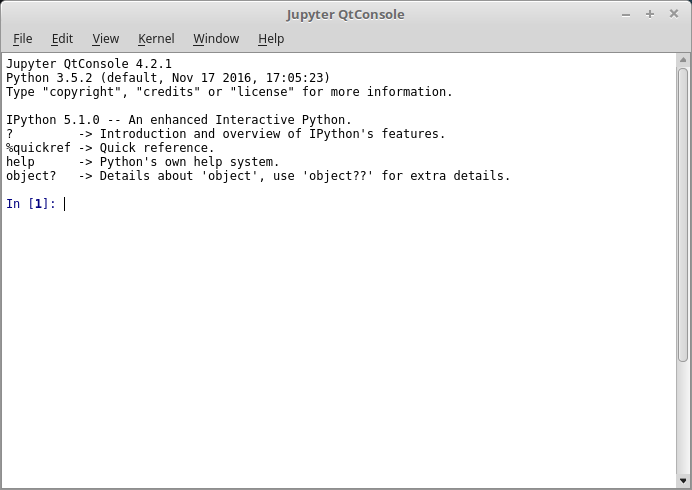
\includegraphics{Figs/Jupyter_QtConsole.png}
\caption{qtconsole}
\end{figure}

    \section{Jupyter Notebook}\label{jupyter-notebook}

Ao longo do tempo, o projeto IPython cresceu para incluir vários
componentes, incluindo:

\begin{itemize}
\tightlist
\item
  Um shell interativo
\item
  Um protocolo REPL
\item
  Um documento de caderno fromat
\item
  Uma ferramenta de conversão de documentos do notebook
\item
  Uma ferramenta de criação de notebooks baseada na web
\item
  Ferramentas para a construção de interface interativa (widgets)
\item
  Python paralelo interativo
\end{itemize}

Como cada componente evoluiu, vários tinham crescido ao ponto que eles
warrented projetos de seus próprios. Por exemplo, peças como o notebook
e o protocolo não são nem mesmo específicas do Python. Como resultado, a
equipe do IPython criou o Projeto Jupyter, que é a nova casa de projetos
agnósticos de linguagem que começou como parte do IPython, como o
notebook no qual você está lendo este texto.

O notebook HTML que faz parte do projeto Jupyter suporta ** visualização
de dados interativos ** e fácil de alto desempenho ** computação
paralela **.

    \begin{Verbatim}[commandchars=\\\{\}]
{\color{incolor}In [{\color{incolor}23}]:} \PY{k+kn}{import} \PY{n+nn}{matplotlib}\PY{n+nn}{.}\PY{n+nn}{pyplot} \PY{k}{as} \PY{n+nn}{plt}
         \PY{n}{plt}\PY{o}{.}\PY{n}{style}\PY{o}{.}\PY{n}{use}\PY{p}{(}\PY{l+s+s1}{\PYZsq{}}\PY{l+s+s1}{fivethirtyeight}\PY{l+s+s1}{\PYZsq{}}\PY{p}{)}
         
         \PY{k}{def} \PY{n+nf}{f}\PY{p}{(}\PY{n}{x}\PY{p}{)}\PY{p}{:}
             \PY{k}{return} \PY{n}{x}\PY{o}{*}\PY{o}{*}\PY{l+m+mi}{2}\PY{o}{\PYZhy{}}\PY{l+m+mi}{10}\PY{o}{*}\PY{n}{x}
         \PY{c+c1}{\PYZsh{}(x\PYZhy{}3)*(x\PYZhy{}5)*(x\PYZhy{}7)+85}
         
         \PY{k+kn}{import} \PY{n+nn}{numpy} \PY{k}{as} \PY{n+nn}{np}
         \PY{n}{x0} \PY{o}{=} \PY{o}{\PYZhy{}}\PY{l+m+mi}{10}        \PY{c+c1}{\PYZsh{} origem}
         \PY{n}{xf} \PY{o}{=} \PY{l+m+mi}{10}         \PY{c+c1}{\PYZsh{} fim do intervalo}
         \PY{n}{n}  \PY{o}{=} \PY{l+m+mi}{200}        \PY{c+c1}{\PYZsh{} número de pontos que se discretiza o intervalo (x0,xf)}
         \PY{n}{x} \PY{o}{=} \PY{n}{np}\PY{o}{.}\PY{n}{linspace}\PY{p}{(}\PY{n}{x0}\PY{p}{,} \PY{n}{xf}\PY{p}{,} \PY{n}{n}\PY{p}{)}
         \PY{n}{y} \PY{o}{=} \PY{n}{f}\PY{p}{(}\PY{n}{x}\PY{p}{)}
         \PY{n}{plt}\PY{o}{.}\PY{n}{plot}\PY{p}{(}\PY{n}{x}\PY{p}{,}\PY{n}{y}\PY{p}{)}
\end{Verbatim}


\begin{Verbatim}[commandchars=\\\{\}]
{\color{outcolor}Out[{\color{outcolor}23}]:} [<matplotlib.lines.Line2D at 0x7f255c18e550>]
\end{Verbatim}
            
    \begin{center}
    \adjustimage{max size={0.9\linewidth}{0.9\paperheight}}{01-Instalacao-e-configuracao-do-IPython-e-Jupyter_files/01-Instalacao-e-configuracao-do-IPython-e-Jupyter_53_1.png}
    \end{center}
    { \hspace*{\fill} \\}
    
    \begin{Verbatim}[commandchars=\\\{\}]
{\color{incolor}In [{\color{incolor}24}]:} \PY{k}{def} \PY{n+nf}{g}\PY{p}{(}\PY{n}{x}\PY{p}{)}\PY{p}{:}
             \PY{k}{return} \PY{n}{x}\PY{o}{*}\PY{o}{*}\PY{l+m+mi}{4} \PY{o}{\PYZhy{}}\PY{l+m+mi}{3}\PY{o}{*}\PY{n}{x}\PY{o}{*}\PY{o}{*}\PY{l+m+mi}{2} \PY{o}{+}\PY{l+m+mi}{4}\PY{o}{*}\PY{n}{x} \PY{o}{\PYZhy{}}\PY{n}{x} \PY{o}{+}\PY{l+m+mi}{2}
         
         \PY{n}{x} \PY{o}{=} \PY{n}{np}\PY{o}{.}\PY{n}{linspace}\PY{p}{(}\PY{o}{\PYZhy{}}\PY{l+m+mi}{10}\PY{p}{,} \PY{l+m+mi}{10}\PY{p}{,} \PY{l+m+mi}{100}\PY{p}{)}
         \PY{n}{y} \PY{o}{=} \PY{n}{g}\PY{p}{(}\PY{n}{x}\PY{p}{)}
         \PY{n}{plt}\PY{o}{.}\PY{n}{plot}\PY{p}{(}\PY{n}{x}\PY{p}{,}\PY{n}{y}\PY{p}{)}
\end{Verbatim}


\begin{Verbatim}[commandchars=\\\{\}]
{\color{outcolor}Out[{\color{outcolor}24}]:} [<matplotlib.lines.Line2D at 0x7f255a0f7860>]
\end{Verbatim}
            
    \begin{center}
    \adjustimage{max size={0.9\linewidth}{0.9\paperheight}}{01-Instalacao-e-configuracao-do-IPython-e-Jupyter_files/01-Instalacao-e-configuracao-do-IPython-e-Jupyter_54_1.png}
    \end{center}
    { \hspace*{\fill} \\}
    
    O notebook permite documentar seu fluxo de trabalho usando HTML ou
Markdown.

O Jupyter Notebook consiste em dois componentes relacionados:

\begin{itemize}
\tightlist
\item
  Um formato de documento JSON baseado em Notebook para gravação e
  distribuição de código Python e texto rico.
\item
  subb1
\item
  sub2
\item
  Uma interface de usuário baseada na web para a criação e execução de
  documentos do notebook.
\end{itemize}

O Notebook pode ser usado iniciando o servidor Notebook com o comando:

\begin{quote}
\$ ipython3 notebook
\end{quote}

Isso inicia um \textbf{mecanismo IPython}, que é uma instância Python
que leva comandos Python através de uma conexão de rede.

O \textbf{controlador IPython} fornece uma interface para trabalhar com
um conjunto de mecanismos, aos quais um ou mais \textbf{clientes
IPython} podem se conectar.

O Notebook dá-lhe tudo o que um navegador lhe dá. Por exemplo, você pode
incorporar imagens, vídeos ou sites inteiros.

    \begin{Verbatim}[commandchars=\\\{\}]
{\color{incolor}In [{\color{incolor}25}]:} \PY{k+kn}{from} \PY{n+nn}{IPython}\PY{n+nn}{.}\PY{n+nn}{display} \PY{k}{import} \PY{n}{HTML}
         \PY{n}{HTML}\PY{p}{(}\PY{l+s+s2}{\PYZdq{}}\PY{l+s+s2}{\PYZlt{}iframe src=http://jupyter.org/ width=700 height=350\PYZgt{}\PYZlt{}/iframe\PYZgt{}}\PY{l+s+s2}{\PYZdq{}}\PY{p}{)}
\end{Verbatim}


\begin{Verbatim}[commandchars=\\\{\}]
{\color{outcolor}Out[{\color{outcolor}25}]:} <IPython.core.display.HTML object>
\end{Verbatim}
            
    \begin{Verbatim}[commandchars=\\\{\}]
{\color{incolor}In [{\color{incolor}26}]:} \PY{k+kn}{from} \PY{n+nn}{IPython}\PY{n+nn}{.}\PY{n+nn}{display} \PY{k}{import} \PY{n}{YouTubeVideo}
         \PY{n}{YouTubeVideo}\PY{p}{(}\PY{l+s+s2}{\PYZdq{}}\PY{l+s+s2}{rl5DaFbLc60}\PY{l+s+s2}{\PYZdq{}}\PY{p}{)}
\end{Verbatim}

\texttt{\color{outcolor}Out[{\color{outcolor}26}]:}
    
    \begin{center}
    \adjustimage{max size={0.9\linewidth}{0.9\paperheight}}{01-Instalacao-e-configuracao-do-IPython-e-Jupyter_files/01-Instalacao-e-configuracao-do-IPython-e-Jupyter_57_0.jpeg}
    \end{center}
    { \hspace*{\fill} \\}
    

    \subsubsection{Código Remoto}\label{cuxf3digo-remoto}

Use \texttt{\%load} para adicionar um código remoto

    \begin{Verbatim}[commandchars=\\\{\}]
{\color{incolor}In [{\color{incolor}27}]:} \PY{c+c1}{\PYZsh{} \PYZpc{}load http://matplotlib.org/\PYZus{}downloads/polar\PYZus{}legend.py}
         \PY{l+s+sd}{\PYZdq{}\PYZdq{}\PYZdq{}}
         \PY{l+s+sd}{============}
         \PY{l+s+sd}{Polar Legend}
         \PY{l+s+sd}{============}
         
         \PY{l+s+sd}{Demo of a legend on a polar\PYZhy{}axis plot.}
         \PY{l+s+sd}{\PYZdq{}\PYZdq{}\PYZdq{}}
         \PY{k+kn}{import} \PY{n+nn}{numpy} \PY{k}{as} \PY{n+nn}{np}
         \PY{k+kn}{from} \PY{n+nn}{matplotlib}\PY{n+nn}{.}\PY{n+nn}{pyplot} \PY{k}{import} \PY{n}{figure}\PY{p}{,} \PY{n}{show}\PY{p}{,} \PY{n}{rc}
         
         \PY{c+c1}{\PYZsh{} radar green, solid grid lines}
         \PY{n}{rc}\PY{p}{(}\PY{l+s+s1}{\PYZsq{}}\PY{l+s+s1}{grid}\PY{l+s+s1}{\PYZsq{}}\PY{p}{,} \PY{n}{color}\PY{o}{=}\PY{l+s+s1}{\PYZsq{}}\PY{l+s+s1}{\PYZsh{}316931}\PY{l+s+s1}{\PYZsq{}}\PY{p}{,} \PY{n}{linewidth}\PY{o}{=}\PY{l+m+mi}{1}\PY{p}{,} \PY{n}{linestyle}\PY{o}{=}\PY{l+s+s1}{\PYZsq{}}\PY{l+s+s1}{\PYZhy{}}\PY{l+s+s1}{\PYZsq{}}\PY{p}{)}
         \PY{n}{rc}\PY{p}{(}\PY{l+s+s1}{\PYZsq{}}\PY{l+s+s1}{xtick}\PY{l+s+s1}{\PYZsq{}}\PY{p}{,} \PY{n}{labelsize}\PY{o}{=}\PY{l+m+mi}{15}\PY{p}{)}
         \PY{n}{rc}\PY{p}{(}\PY{l+s+s1}{\PYZsq{}}\PY{l+s+s1}{ytick}\PY{l+s+s1}{\PYZsq{}}\PY{p}{,} \PY{n}{labelsize}\PY{o}{=}\PY{l+m+mi}{15}\PY{p}{)}
         
         \PY{c+c1}{\PYZsh{} force square figure and square axes looks better for polar, IMO}
         \PY{n}{fig} \PY{o}{=} \PY{n}{figure}\PY{p}{(}\PY{n}{figsize}\PY{o}{=}\PY{p}{(}\PY{l+m+mi}{8}\PY{p}{,} \PY{l+m+mi}{8}\PY{p}{)}\PY{p}{)}
         \PY{n}{ax} \PY{o}{=} \PY{n}{fig}\PY{o}{.}\PY{n}{add\PYZus{}axes}\PY{p}{(}\PY{p}{[}\PY{l+m+mf}{0.1}\PY{p}{,} \PY{l+m+mf}{0.1}\PY{p}{,} \PY{l+m+mf}{0.8}\PY{p}{,} \PY{l+m+mf}{0.8}\PY{p}{]}\PY{p}{,}
                           \PY{n}{projection}\PY{o}{=}\PY{l+s+s1}{\PYZsq{}}\PY{l+s+s1}{polar}\PY{l+s+s1}{\PYZsq{}}\PY{p}{,} \PY{n}{facecolor}\PY{o}{=}\PY{l+s+s1}{\PYZsq{}}\PY{l+s+s1}{\PYZsh{}d5de9c}\PY{l+s+s1}{\PYZsq{}}\PY{p}{)}
         
         \PY{n}{r} \PY{o}{=} \PY{n}{np}\PY{o}{.}\PY{n}{arange}\PY{p}{(}\PY{l+m+mi}{0}\PY{p}{,} \PY{l+m+mf}{3.0}\PY{p}{,} \PY{l+m+mf}{0.01}\PY{p}{)}
         \PY{n}{theta} \PY{o}{=} \PY{l+m+mi}{2} \PY{o}{*} \PY{n}{np}\PY{o}{.}\PY{n}{pi} \PY{o}{*} \PY{n}{r}
         \PY{n}{ax}\PY{o}{.}\PY{n}{plot}\PY{p}{(}\PY{n}{theta}\PY{p}{,} \PY{n}{r}\PY{p}{,} \PY{n}{color}\PY{o}{=}\PY{l+s+s1}{\PYZsq{}}\PY{l+s+s1}{\PYZsh{}ee8d18}\PY{l+s+s1}{\PYZsq{}}\PY{p}{,} \PY{n}{lw}\PY{o}{=}\PY{l+m+mi}{3}\PY{p}{,} \PY{n}{label}\PY{o}{=}\PY{l+s+s1}{\PYZsq{}}\PY{l+s+s1}{a line}\PY{l+s+s1}{\PYZsq{}}\PY{p}{)}
         \PY{n}{ax}\PY{o}{.}\PY{n}{plot}\PY{p}{(}\PY{l+m+mf}{0.5} \PY{o}{*} \PY{n}{theta}\PY{p}{,} \PY{n}{r}\PY{p}{,} \PY{n}{color}\PY{o}{=}\PY{l+s+s1}{\PYZsq{}}\PY{l+s+s1}{blue}\PY{l+s+s1}{\PYZsq{}}\PY{p}{,} \PY{n}{ls}\PY{o}{=}\PY{l+s+s1}{\PYZsq{}}\PY{l+s+s1}{\PYZhy{}\PYZhy{}}\PY{l+s+s1}{\PYZsq{}}\PY{p}{,} \PY{n}{lw}\PY{o}{=}\PY{l+m+mi}{3}\PY{p}{,} \PY{n}{label}\PY{o}{=}\PY{l+s+s1}{\PYZsq{}}\PY{l+s+s1}{another line}\PY{l+s+s1}{\PYZsq{}}\PY{p}{)}
         \PY{n}{ax}\PY{o}{.}\PY{n}{legend}\PY{p}{(}\PY{p}{)}
         
         \PY{n}{show}\PY{p}{(}\PY{p}{)}
\end{Verbatim}


    \begin{center}
    \adjustimage{max size={0.9\linewidth}{0.9\paperheight}}{01-Instalacao-e-configuracao-do-IPython-e-Jupyter_files/01-Instalacao-e-configuracao-do-IPython-e-Jupyter_59_0.png}
    \end{center}
    { \hspace*{\fill} \\}
    
    \begin{Verbatim}[commandchars=\\\{\}]
{\color{incolor}In [{\color{incolor}28}]:} \PY{c+c1}{\PYZsh{} \PYZpc{}load http://matplotlib.org/mpl\PYZus{}examples/shapes\PYZus{}and\PYZus{}collections/scatter\PYZus{}demo.py}
         \PY{l+s+sd}{\PYZdq{}\PYZdq{}\PYZdq{}}
         \PY{l+s+sd}{Simple demo of a scatter plot.}
         \PY{l+s+sd}{\PYZdq{}\PYZdq{}\PYZdq{}}
         \PY{k+kn}{import} \PY{n+nn}{numpy} \PY{k}{as} \PY{n+nn}{np}
         \PY{k+kn}{import} \PY{n+nn}{matplotlib}\PY{n+nn}{.}\PY{n+nn}{pyplot} \PY{k}{as} \PY{n+nn}{plt}
         
         
         \PY{n}{N} \PY{o}{=} \PY{l+m+mi}{50}
         \PY{n}{x} \PY{o}{=} \PY{n}{np}\PY{o}{.}\PY{n}{random}\PY{o}{.}\PY{n}{rand}\PY{p}{(}\PY{n}{N}\PY{p}{)}
         \PY{n}{y} \PY{o}{=} \PY{n}{np}\PY{o}{.}\PY{n}{random}\PY{o}{.}\PY{n}{rand}\PY{p}{(}\PY{n}{N}\PY{p}{)}
         \PY{n}{colors} \PY{o}{=} \PY{n}{np}\PY{o}{.}\PY{n}{random}\PY{o}{.}\PY{n}{rand}\PY{p}{(}\PY{n}{N}\PY{p}{)}
         \PY{n}{area} \PY{o}{=} \PY{n}{np}\PY{o}{.}\PY{n}{pi} \PY{o}{*} \PY{p}{(}\PY{l+m+mi}{15} \PY{o}{*} \PY{n}{np}\PY{o}{.}\PY{n}{random}\PY{o}{.}\PY{n}{rand}\PY{p}{(}\PY{n}{N}\PY{p}{)}\PY{p}{)}\PY{o}{*}\PY{o}{*}\PY{l+m+mi}{2}  \PY{c+c1}{\PYZsh{} 0 to 15 point radii}
         
         \PY{n}{plt}\PY{o}{.}\PY{n}{scatter}\PY{p}{(}\PY{n}{x}\PY{p}{,} \PY{n}{y}\PY{p}{,} \PY{n}{s}\PY{o}{=}\PY{n}{area}\PY{p}{,} \PY{n}{c}\PY{o}{=}\PY{n}{colors}\PY{p}{,} \PY{n}{alpha}\PY{o}{=}\PY{l+m+mf}{0.5}\PY{p}{)}
         \PY{n}{plt}\PY{o}{.}\PY{n}{show}\PY{p}{(}\PY{p}{)}
\end{Verbatim}


    \begin{center}
    \adjustimage{max size={0.9\linewidth}{0.9\paperheight}}{01-Instalacao-e-configuracao-do-IPython-e-Jupyter_files/01-Instalacao-e-configuracao-do-IPython-e-Jupyter_60_0.png}
    \end{center}
    { \hspace*{\fill} \\}
    
    \begin{Verbatim}[commandchars=\\\{\}]
{\color{incolor}In [{\color{incolor}29}]:} \PY{c+c1}{\PYZsh{} \PYZpc{}load http://matplotlib.org/examples/frontpage/plot\PYZus{}contour.py}
         \PY{l+s+sd}{\PYZdq{}\PYZdq{}\PYZdq{}}
         \PY{l+s+sd}{=========================}
         \PY{l+s+sd}{Frontpage contour example}
         \PY{l+s+sd}{=========================}
         
         \PY{l+s+sd}{This example reproduces the frontpage contour example.}
         \PY{l+s+sd}{\PYZdq{}\PYZdq{}\PYZdq{}}
         
         \PY{k+kn}{import} \PY{n+nn}{matplotlib}\PY{n+nn}{.}\PY{n+nn}{pyplot} \PY{k}{as} \PY{n+nn}{plt}
         \PY{k+kn}{import} \PY{n+nn}{numpy} \PY{k}{as} \PY{n+nn}{np}
         \PY{k+kn}{from} \PY{n+nn}{matplotlib} \PY{k}{import} \PY{n}{mlab}\PY{p}{,} \PY{n}{cm}
         
         \PY{n}{extent} \PY{o}{=} \PY{p}{(}\PY{o}{\PYZhy{}}\PY{l+m+mi}{3}\PY{p}{,} \PY{l+m+mi}{3}\PY{p}{,} \PY{o}{\PYZhy{}}\PY{l+m+mi}{3}\PY{p}{,} \PY{l+m+mi}{3}\PY{p}{)}
         
         \PY{n}{delta} \PY{o}{=} \PY{l+m+mf}{0.1}
         \PY{n}{x} \PY{o}{=} \PY{n}{np}\PY{o}{.}\PY{n}{arange}\PY{p}{(}\PY{o}{\PYZhy{}}\PY{l+m+mf}{3.0}\PY{p}{,} \PY{l+m+mf}{4.001}\PY{p}{,} \PY{n}{delta}\PY{p}{)}
         \PY{n}{y} \PY{o}{=} \PY{n}{np}\PY{o}{.}\PY{n}{arange}\PY{p}{(}\PY{o}{\PYZhy{}}\PY{l+m+mf}{4.0}\PY{p}{,} \PY{l+m+mf}{3.001}\PY{p}{,} \PY{n}{delta}\PY{p}{)}
         \PY{n}{X}\PY{p}{,} \PY{n}{Y} \PY{o}{=} \PY{n}{np}\PY{o}{.}\PY{n}{meshgrid}\PY{p}{(}\PY{n}{x}\PY{p}{,} \PY{n}{y}\PY{p}{)}
         \PY{n}{Z1} \PY{o}{=} \PY{n}{mlab}\PY{o}{.}\PY{n}{bivariate\PYZus{}normal}\PY{p}{(}\PY{n}{X}\PY{p}{,} \PY{n}{Y}\PY{p}{,} \PY{l+m+mf}{1.0}\PY{p}{,} \PY{l+m+mf}{1.0}\PY{p}{,} \PY{l+m+mf}{0.0}\PY{p}{,} \PY{o}{\PYZhy{}}\PY{l+m+mf}{0.5}\PY{p}{)}
         \PY{n}{Z2} \PY{o}{=} \PY{n}{mlab}\PY{o}{.}\PY{n}{bivariate\PYZus{}normal}\PY{p}{(}\PY{n}{X}\PY{p}{,} \PY{n}{Y}\PY{p}{,} \PY{l+m+mf}{1.5}\PY{p}{,} \PY{l+m+mf}{0.5}\PY{p}{,} \PY{l+m+mi}{1}\PY{p}{,} \PY{l+m+mi}{1}\PY{p}{)}
         \PY{n}{Z} \PY{o}{=} \PY{p}{(}\PY{n}{Z1} \PY{o}{\PYZhy{}} \PY{n}{Z2}\PY{p}{)} \PY{o}{*} \PY{l+m+mi}{10}
         
         \PY{n}{levels} \PY{o}{=} \PY{n}{np}\PY{o}{.}\PY{n}{linspace}\PY{p}{(}\PY{o}{\PYZhy{}}\PY{l+m+mf}{2.0}\PY{p}{,} \PY{l+m+mf}{1.601}\PY{p}{,} \PY{l+m+mi}{40}\PY{p}{)}
         \PY{n}{norm} \PY{o}{=} \PY{n}{cm}\PY{o}{.}\PY{n}{colors}\PY{o}{.}\PY{n}{Normalize}\PY{p}{(}\PY{n}{vmax}\PY{o}{=}\PY{n+nb}{abs}\PY{p}{(}\PY{n}{Z}\PY{p}{)}\PY{o}{.}\PY{n}{max}\PY{p}{(}\PY{p}{)}\PY{p}{,} \PY{n}{vmin}\PY{o}{=}\PY{o}{\PYZhy{}}\PY{n+nb}{abs}\PY{p}{(}\PY{n}{Z}\PY{p}{)}\PY{o}{.}\PY{n}{max}\PY{p}{(}\PY{p}{)}\PY{p}{)}
         
         \PY{n}{fig}\PY{p}{,} \PY{n}{ax} \PY{o}{=} \PY{n}{plt}\PY{o}{.}\PY{n}{subplots}\PY{p}{(}\PY{p}{)}
         \PY{n}{cset1} \PY{o}{=} \PY{n}{ax}\PY{o}{.}\PY{n}{contourf}\PY{p}{(}
             \PY{n}{X}\PY{p}{,} \PY{n}{Y}\PY{p}{,} \PY{n}{Z}\PY{p}{,} \PY{n}{levels}\PY{p}{,}
             \PY{n}{norm}\PY{o}{=}\PY{n}{norm}\PY{p}{)}
         \PY{n}{ax}\PY{o}{.}\PY{n}{set\PYZus{}xlim}\PY{p}{(}\PY{o}{\PYZhy{}}\PY{l+m+mi}{3}\PY{p}{,} \PY{l+m+mi}{3}\PY{p}{)}
         \PY{n}{ax}\PY{o}{.}\PY{n}{set\PYZus{}ylim}\PY{p}{(}\PY{o}{\PYZhy{}}\PY{l+m+mi}{3}\PY{p}{,} \PY{l+m+mi}{3}\PY{p}{)}
         \PY{n}{ax}\PY{o}{.}\PY{n}{set\PYZus{}xticks}\PY{p}{(}\PY{p}{[}\PY{p}{]}\PY{p}{)}
         \PY{n}{ax}\PY{o}{.}\PY{n}{set\PYZus{}yticks}\PY{p}{(}\PY{p}{[}\PY{p}{]}\PY{p}{)}
         \PY{n}{fig}\PY{o}{.}\PY{n}{savefig}\PY{p}{(}\PY{l+s+s2}{\PYZdq{}}\PY{l+s+s2}{contour\PYZus{}frontpage.png}\PY{l+s+s2}{\PYZdq{}}\PY{p}{,} \PY{n}{dpi}\PY{o}{=}\PY{l+m+mi}{300}\PY{p}{)}  \PY{c+c1}{\PYZsh{} results in 160x120 px image}
\end{Verbatim}


    \begin{center}
    \adjustimage{max size={0.9\linewidth}{0.9\paperheight}}{01-Instalacao-e-configuracao-do-IPython-e-Jupyter_files/01-Instalacao-e-configuracao-do-IPython-e-Jupyter_61_0.png}
    \end{center}
    { \hspace*{\fill} \\}
    
    \begin{Verbatim}[commandchars=\\\{\}]
{\color{incolor}In [{\color{incolor} }]:} \PY{o}{\PYZpc{}}\PY{k}{matplotlib} qt5
\end{Verbatim}


    \begin{Verbatim}[commandchars=\\\{\}]
{\color{incolor}In [{\color{incolor}30}]:} \PY{c+c1}{\PYZsh{} \PYZpc{}load http://matplotlib.org/mpl\PYZus{}examples/mplot3d/contour3d\PYZus{}demo3.py}
         \PY{c+c1}{\PYZsh{} Para fazer o gráfico em uma janela habilite:}
         \PY{c+c1}{\PYZsh{} \PYZpc{}matplotlib qt}
         \PY{k+kn}{from} \PY{n+nn}{mpl\PYZus{}toolkits}\PY{n+nn}{.}\PY{n+nn}{mplot3d} \PY{k}{import} \PY{n}{axes3d}
         \PY{k+kn}{import} \PY{n+nn}{matplotlib}\PY{n+nn}{.}\PY{n+nn}{pyplot} \PY{k}{as} \PY{n+nn}{plt}
         \PY{k+kn}{from} \PY{n+nn}{matplotlib} \PY{k}{import} \PY{n}{cm}
         
         \PY{n}{fig} \PY{o}{=} \PY{n}{plt}\PY{o}{.}\PY{n}{figure}\PY{p}{(}\PY{p}{)}
         \PY{n}{ax} \PY{o}{=} \PY{n}{fig}\PY{o}{.}\PY{n}{gca}\PY{p}{(}\PY{n}{projection}\PY{o}{=}\PY{l+s+s1}{\PYZsq{}}\PY{l+s+s1}{3d}\PY{l+s+s1}{\PYZsq{}}\PY{p}{)}
         \PY{n}{X}\PY{p}{,} \PY{n}{Y}\PY{p}{,} \PY{n}{Z} \PY{o}{=} \PY{n}{axes3d}\PY{o}{.}\PY{n}{get\PYZus{}test\PYZus{}data}\PY{p}{(}\PY{l+m+mf}{0.02}\PY{p}{)}
         \PY{n}{ax}\PY{o}{.}\PY{n}{plot\PYZus{}surface}\PY{p}{(}\PY{n}{X}\PY{p}{,} \PY{n}{Y}\PY{p}{,} \PY{n}{Z}\PY{p}{,} \PY{n}{rstride}\PY{o}{=}\PY{l+m+mi}{10}\PY{p}{,} \PY{n}{cstride}\PY{o}{=}\PY{l+m+mi}{10}\PY{p}{,} \PY{n}{alpha}\PY{o}{=}\PY{l+m+mf}{0.3}\PY{p}{)}
         \PY{n}{cset} \PY{o}{=} \PY{n}{ax}\PY{o}{.}\PY{n}{contour}\PY{p}{(}\PY{n}{X}\PY{p}{,} \PY{n}{Y}\PY{p}{,} \PY{n}{Z}\PY{p}{,} \PY{n}{zdir}\PY{o}{=}\PY{l+s+s1}{\PYZsq{}}\PY{l+s+s1}{z}\PY{l+s+s1}{\PYZsq{}}\PY{p}{,} \PY{n}{offset}\PY{o}{=}\PY{o}{\PYZhy{}}\PY{l+m+mi}{100}\PY{p}{,} \PY{n}{cmap}\PY{o}{=}\PY{n}{cm}\PY{o}{.}\PY{n}{coolwarm}\PY{p}{)}
         \PY{n}{cset} \PY{o}{=} \PY{n}{ax}\PY{o}{.}\PY{n}{contour}\PY{p}{(}\PY{n}{X}\PY{p}{,} \PY{n}{Y}\PY{p}{,} \PY{n}{Z}\PY{p}{,} \PY{n}{zdir}\PY{o}{=}\PY{l+s+s1}{\PYZsq{}}\PY{l+s+s1}{x}\PY{l+s+s1}{\PYZsq{}}\PY{p}{,} \PY{n}{offset}\PY{o}{=}\PY{o}{\PYZhy{}}\PY{l+m+mi}{40}\PY{p}{,} \PY{n}{cmap}\PY{o}{=}\PY{n}{cm}\PY{o}{.}\PY{n}{coolwarm}\PY{p}{)}
         \PY{n}{cset} \PY{o}{=} \PY{n}{ax}\PY{o}{.}\PY{n}{contour}\PY{p}{(}\PY{n}{X}\PY{p}{,} \PY{n}{Y}\PY{p}{,} \PY{n}{Z}\PY{p}{,} \PY{n}{zdir}\PY{o}{=}\PY{l+s+s1}{\PYZsq{}}\PY{l+s+s1}{y}\PY{l+s+s1}{\PYZsq{}}\PY{p}{,} \PY{n}{offset}\PY{o}{=}\PY{l+m+mi}{40}\PY{p}{,} \PY{n}{cmap}\PY{o}{=}\PY{n}{cm}\PY{o}{.}\PY{n}{coolwarm}\PY{p}{)}
         
         \PY{n}{ax}\PY{o}{.}\PY{n}{set\PYZus{}xlabel}\PY{p}{(}\PY{l+s+s1}{\PYZsq{}}\PY{l+s+s1}{X}\PY{l+s+s1}{\PYZsq{}}\PY{p}{)}
         \PY{n}{ax}\PY{o}{.}\PY{n}{set\PYZus{}xlim}\PY{p}{(}\PY{o}{\PYZhy{}}\PY{l+m+mi}{40}\PY{p}{,} \PY{l+m+mi}{40}\PY{p}{)}
         \PY{n}{ax}\PY{o}{.}\PY{n}{set\PYZus{}ylabel}\PY{p}{(}\PY{l+s+s1}{\PYZsq{}}\PY{l+s+s1}{Y}\PY{l+s+s1}{\PYZsq{}}\PY{p}{)}
         \PY{n}{ax}\PY{o}{.}\PY{n}{set\PYZus{}ylim}\PY{p}{(}\PY{o}{\PYZhy{}}\PY{l+m+mi}{40}\PY{p}{,} \PY{l+m+mi}{40}\PY{p}{)}
         \PY{n}{ax}\PY{o}{.}\PY{n}{set\PYZus{}zlabel}\PY{p}{(}\PY{l+s+s1}{\PYZsq{}}\PY{l+s+s1}{Z}\PY{l+s+s1}{\PYZsq{}}\PY{p}{)}
         \PY{n}{ax}\PY{o}{.}\PY{n}{set\PYZus{}zlim}\PY{p}{(}\PY{o}{\PYZhy{}}\PY{l+m+mi}{100}\PY{p}{,} \PY{l+m+mi}{100}\PY{p}{)}
         
         \PY{n}{plt}\PY{o}{.}\PY{n}{show}\PY{p}{(}\PY{p}{)}
\end{Verbatim}


    \begin{center}
    \adjustimage{max size={0.9\linewidth}{0.9\paperheight}}{01-Instalacao-e-configuracao-do-IPython-e-Jupyter_files/01-Instalacao-e-configuracao-do-IPython-e-Jupyter_63_0.png}
    \end{center}
    { \hspace*{\fill} \\}
    
    \subsubsection{Suporte ao Mathjax}\label{suporte-ao-mathjax}

Mathjax é uma implementação javascript \(\alpha\) do LaTeX que permite
que as equações sejam incorporadas em HTML. Por exemplo, esta marcação:

\begin{verbatim}
"""$$ \int_{a}^{b} f(x)\, dx \approx \frac{1}{2} \sum_{k=1}^{N} \left( x_{k} - x_{k-1} \right) \left( f(x_{k}) + f(x_{k-1}) \right). $$"""
\end{verbatim}

torna-se:

\[
\int_{a}^{b} f(x)\, dx \approx \frac{1}{2} \sum_{k=1}^{N} \left( x_{k} - x_{k-1} \right) \left( f(x_{k}) + f(x_{k-1}) \right).
\]

    \subsection{Suporte SymPy}\label{suporte-sympy}

SymPy é uma biblioteca Python para cálculo simbólico mathematics. Ela
suporta:

\begin{itemize}
\tightlist
\item
  polinômios
\item
  cálculo
\item
  resolvendo equações
\item
  matemática discreta
\item
  matrizes
\end{itemize}

    \begin{Verbatim}[commandchars=\\\{\}]
{\color{incolor}In [{\color{incolor}31}]:} \PY{k+kn}{from} \PY{n+nn}{sympy} \PY{k}{import} \PY{o}{*}
         \PY{n}{init\PYZus{}printing}\PY{p}{(}\PY{p}{)}
         \PY{n}{x}\PY{p}{,} \PY{n}{y} \PY{o}{=} \PY{n}{symbols}\PY{p}{(}\PY{l+s+s2}{\PYZdq{}}\PY{l+s+s2}{x y}\PY{l+s+s2}{\PYZdq{}}\PY{p}{)}
\end{Verbatim}


    \begin{Verbatim}[commandchars=\\\{\}]
{\color{incolor}In [{\color{incolor}32}]:} \PY{n}{eq} \PY{o}{=} \PY{p}{(}\PY{p}{(}\PY{n}{x}\PY{o}{+}\PY{n}{y}\PY{p}{)}\PY{o}{*}\PY{o}{*}\PY{l+m+mi}{3} \PY{o}{*} \PY{p}{(}\PY{n}{x}\PY{o}{+}\PY{l+m+mi}{1}\PY{p}{)}\PY{p}{)}
         \PY{n}{eq}
\end{Verbatim}

\texttt{\color{outcolor}Out[{\color{outcolor}32}]:}
    
    $$\left(x + 1\right) \left(x + y\right)^{3}$$

    

    \begin{Verbatim}[commandchars=\\\{\}]
{\color{incolor}In [{\color{incolor}33}]:} \PY{n}{expand}\PY{p}{(}\PY{n}{eq}\PY{p}{)}
\end{Verbatim}

\texttt{\color{outcolor}Out[{\color{outcolor}33}]:}
    
    $$x^{4} + 3 x^{3} y + x^{3} + 3 x^{2} y^{2} + 3 x^{2} y + x y^{3} + 3 x y^{2} + y^{3}$$

    

    \begin{Verbatim}[commandchars=\\\{\}]
{\color{incolor}In [{\color{incolor}34}]:} \PY{p}{(}\PY{l+m+mi}{1}\PY{o}{/}\PY{n}{cos}\PY{p}{(}\PY{n}{x}\PY{p}{)}\PY{p}{)}\PY{o}{.}\PY{n}{series}\PY{p}{(}\PY{n}{x}\PY{p}{,} \PY{l+m+mi}{0}\PY{p}{,} \PY{l+m+mi}{12}\PY{p}{)}
\end{Verbatim}

\texttt{\color{outcolor}Out[{\color{outcolor}34}]:}
    
    $$1 + \frac{x^{2}}{2} + \frac{5 x^{4}}{24} + \frac{61 x^{6}}{720} + \frac{277 x^{8}}{8064} + \frac{50521 x^{10}}{3628800} + \mathcal{O}\left(x^{12}\right)$$

    

    \begin{Verbatim}[commandchars=\\\{\}]
{\color{incolor}In [{\color{incolor}35}]:} \PY{n}{limit}\PY{p}{(}\PY{p}{(}\PY{n}{sin}\PY{p}{(}\PY{n}{x}\PY{p}{)}\PY{o}{\PYZhy{}}\PY{n}{x}\PY{p}{)}\PY{o}{/}\PY{n}{x}\PY{o}{*}\PY{o}{*}\PY{l+m+mi}{3}\PY{p}{,} \PY{n}{x}\PY{p}{,} \PY{l+m+mi}{0}\PY{p}{)}
\end{Verbatim}

\texttt{\color{outcolor}Out[{\color{outcolor}35}]:}
    
    $$- \frac{1}{6}$$

    

    \begin{Verbatim}[commandchars=\\\{\}]
{\color{incolor}In [{\color{incolor}36}]:} \PY{n}{diff}\PY{p}{(}\PY{n}{cos}\PY{p}{(}\PY{n}{x}\PY{o}{*}\PY{o}{*}\PY{l+m+mi}{2}\PY{p}{)}\PY{o}{*}\PY{o}{*}\PY{l+m+mi}{2} \PY{o}{/} \PY{p}{(}\PY{l+m+mi}{1}\PY{o}{+}\PY{n}{x}\PY{p}{)}\PY{p}{,} \PY{n}{x}\PY{p}{)}
\end{Verbatim}

\texttt{\color{outcolor}Out[{\color{outcolor}36}]:}
    
    $$- \frac{4 x \cos{\left (x^{2} \right )}}{x + 1} \sin{\left (x^{2} \right )} - \frac{\cos^{2}{\left (x^{2} \right )}}{\left(x + 1\right)^{2}}$$

    

    \begin{Verbatim}[commandchars=\\\{\}]
{\color{incolor}In [{\color{incolor}37}]:} \PY{n}{integrate}\PY{p}{(}\PY{n}{x}\PY{o}{/}\PY{n}{sqrt}\PY{p}{(}\PY{n}{x}\PY{o}{*}\PY{o}{*}\PY{l+m+mi}{2} \PY{o}{+}\PY{n}{y}\PY{o}{*}\PY{o}{*}\PY{l+m+mi}{2}\PY{p}{)}\PY{p}{,}\PY{n}{x}\PY{p}{)}
\end{Verbatim}

\texttt{\color{outcolor}Out[{\color{outcolor}37}]:}
    
    $$\sqrt{x^{2} + y^{2}}$$

    

    \subsubsection{Funções mágicas}\label{funuxe7uxf5es-muxe1gicas}

O IPython tem um conjunto de "funções mágicas" predefinidas que você
pode chamar com uma sintaxe de estilo de linha de comando. Esses
incluem:

\begin{itemize}
\tightlist
\item
  \texttt{\%run}
\item
  \texttt{\%edit}
\item
  \texttt{\%debug}
\item
  \texttt{\%timeit}
\item
  \texttt{\%paste}
\item
  \texttt{\%load\_ext}
\end{itemize}

    \begin{Verbatim}[commandchars=\\\{\}]
{\color{incolor}In [{\color{incolor} }]:} \PY{o}{\PYZpc{}}\PY{k}{lsmagic}
\end{Verbatim}


    \subsection{Exemplo: O tutor}\label{exemplo-o-tutor}

Para executar o código abaixo você precisa de uuma conexão com a
internet, pois ele irá executar o comando abaixo no site
\href{http://pythontutor.com/}{Python Tutor}. Esse site é muito bom para
aqueles que estão aprendendo uma linguagem de programação, pois ele
linha por linha o que ocorrer na execução de um código. Usando essa
ferramenta é possível visualizar códigos escritos nas seguintes
linguagens: Python2, Python3, Java, JavaScript, TypeScript, Ruby, C, and
C++.

Como exemplo, considere o seguinte código:

    \begin{Verbatim}[commandchars=\\\{\}]
{\color{incolor}In [{\color{incolor}38}]:} \PY{o}{\PYZpc{}\PYZpc{}}\PY{k}{tutor}
         inicio=4
         fim= 13 \PYZsh{} ele sempre vai terminar um passo antes, ou seja, em 12
         passo = 2
         for i in range(inicio,fim,passo):
             print(i)
\end{Verbatim}


    
    \begin{verbatim}
<IPython.lib.display.IFrame at 0x7f2553f60e10>
    \end{verbatim}

    
    Determinando o tempo de execução do código; O comando magic
\texttt{timeit} existe tanto na forma de linha como de célula:

    \begin{Verbatim}[commandchars=\\\{\}]
{\color{incolor}In [{\color{incolor}39}]:} \PY{k+kn}{import} \PY{n+nn}{numpy} \PY{k}{as} \PY{n+nn}{np}
         \PY{o}{\PYZpc{}}\PY{k}{timeit} np.linalg.eigvals(np.random.rand(100,100))
\end{Verbatim}


    \begin{Verbatim}[commandchars=\\\{\}]
13.8 ms ± 1.3 ms per loop (mean ± std. dev. of 7 runs, 100 loops each)

    \end{Verbatim}

    \begin{Verbatim}[commandchars=\\\{\}]
{\color{incolor}In [{\color{incolor}40}]:} \PY{o}{\PYZpc{}\PYZpc{}}\PY{k}{timeit} a = np.random.rand(100, 100)
         np.linalg.eigvals(a)
\end{Verbatim}


    \begin{Verbatim}[commandchars=\\\{\}]
12.5 ms ± 149 µs per loop (mean ± std. dev. of 7 runs, 100 loops each)

    \end{Verbatim}

    O IPython também cria \emph{aliases} para alguns intérpretes comuns,
como bash, ruby, perl, etc.

Estes são todos equivalentes a
\texttt{\%\%script\ \textless{}nome\textgreater{}}

    \begin{Verbatim}[commandchars=\\\{\}]
{\color{incolor}In [{\color{incolor}41}]:} \PY{o}{\PYZpc{}}\PY{o}{\PYZpc{}}\PY{n}{ruby}
         \PY{n+nb}{puts} \PY{l+s+s2}{\PYZdq{}}\PY{l+s+s2}{Hello from Ruby }\PY{l+s+si}{\PYZsh{}\PYZob{}}\PY{n+no}{RUBY\PYZus{}VERSION}\PY{l+s+si}{\PYZcb{}}\PY{l+s+s2}{\PYZdq{}}
\end{Verbatim}


    \begin{Verbatim}[commandchars=\\\{\}]
Hello from Ruby 2.3.1

    \end{Verbatim}

    \begin{Verbatim}[commandchars=\\\{\}]
{\color{incolor}In [{\color{incolor}42}]:} \PYZpc{}\PYZpc{}bash
         \PY{n+nb}{echo} \PY{l+s+s2}{\PYZdq{}}\PY{l+s+s2}{hello from }\PY{n+nv}{\PYZdl{}BASH}\PY{l+s+s2}{\PYZdq{}}
\end{Verbatim}


    \begin{Verbatim}[commandchars=\\\{\}]
hello from /bin/bash

    \end{Verbatim}

    IPython tem uma extensão \texttt{rmagic} que contém algumas funções
mágicas para trabalhar com R via rpy2. Esta extensão pode ser carregada
usando a magia \texttt{\%load\_ext} da seguinte forma:

    \begin{Verbatim}[commandchars=\\\{\}]
{\color{incolor}In [{\color{incolor} }]:} \PY{o}{\PYZpc{}}\PY{k}{load\PYZus{}ext} rpy2.ipython
\end{Verbatim}


    Se o comando anterior gerar um erro, é provável que você não tenha o
módulo \texttt{rpy2} instalado. Você pode instalar isso agora, em uma
nova célula, usando o seguinte código:

\begin{quote}
!sudo apt install python3-rpy2
\end{quote}

Caso não encontre o pacote, vocẽ pode instalar ele usando o seguinte
código:

\begin{quote}
!sudo -H pip3 install rpy2
\end{quote}

    \begin{Verbatim}[commandchars=\\\{\}]
{\color{incolor}In [{\color{incolor}43}]:} \PY{o}{\PYZpc{}}\PY{k}{load\PYZus{}ext} watermark
\end{Verbatim}


    \begin{Verbatim}[commandchars=\\\{\}]
{\color{incolor}In [{\color{incolor}44}]:} \PY{o}{\PYZpc{}}\PY{k}{watermark}
\end{Verbatim}


    \begin{Verbatim}[commandchars=\\\{\}]
2017-11-22T07:52:40-02:00

CPython 3.5.2
IPython 6.2.1

compiler   : GCC 5.4.0 20160609
system     : Linux
release    : 4.10.0-40-generic
machine    : x86\_64
processor  : x86\_64
CPU cores  : 4
interpreter: 64bit

    \end{Verbatim}

    \begin{Verbatim}[commandchars=\\\{\}]
{\color{incolor}In [{\color{incolor}45}]:} \PY{o}{\PYZpc{}}\PY{k}{watermark} \PYZhy{}t \PYZhy{}n \PYZhy{}u \PYZhy{}z
\end{Verbatim}


    \begin{Verbatim}[commandchars=\\\{\}]
last updated: Wed Nov 22 2017 07:52:41 -02

    \end{Verbatim}

    \begin{Verbatim}[commandchars=\\\{\}]
{\color{incolor}In [{\color{incolor}46}]:} \PY{o}{\PYZpc{}}\PY{k}{watermark} \PYZhy{}v \PYZhy{}m \PYZhy{}p numpy,matplotlib,scipy \PYZhy{}g
\end{Verbatim}


    \begin{Verbatim}[commandchars=\\\{\}]
CPython 3.5.2
IPython 6.2.1

numpy 1.13.3
matplotlib 2.1.0
scipy 1.0.0

compiler   : GCC 5.4.0 20160609
system     : Linux
release    : 4.10.0-40-generic
machine    : x86\_64
processor  : x86\_64
CPU cores  : 4
interpreter: 64bit
Git hash   :

    \end{Verbatim}

    \begin{Verbatim}[commandchars=\\\{\}]
{\color{incolor}In [{\color{incolor} }]:} \PY{o}{\PYZpc{}}\PY{k}{watermark}\PY{o}{?}
\end{Verbatim}


    O comando acima retorna a saída:

\begin{verbatim}
 %watermark [-a AUTHOR] [-d] [-n] [-t] [-i] [-z] [-u] [-c CUSTOM_TIME]
                 [-v] [-p PACKAGES] [-h] [-m] [-g] [-r] [-w] [-iv]

IPython magic function to print date/time stamps
and various system information.

optional arguments:
  -a AUTHOR, --author AUTHOR
                        prints author name
  -d, --date            prints current date as YYYY-mm-dd
  -n, --datename        prints date with abbrv. day and month names
  -t, --time            prints current time as HH-MM-SS
  -i, --iso8601         prints the combined date and time including the time
                        zone in the ISO 8601 standard with UTC offset
  -z, --timezone        appends the local time zone
  -u, --updated         appends a string "Last updated: "
  -c CUSTOM_TIME, --custom_time CUSTOM_TIME
                        prints a valid strftime() string
  -v, --python          prints Python and IPython version
  -p PACKAGES, --packages PACKAGES
                        prints versions of specified Python modules and
                        packages
  -h, --hostname        prints the host name
  -m, --machine         prints system and machine info
  -g, --githash         prints current Git commit hash
  -r, --gitrepo         prints current Git remote address
  -w, --watermark       prints the current version of watermark
  -iv, --iversions      prints the name/version of all imported modules
File:      /usr/local/lib/python3.5/dist-packages/watermark/watermark.py
\end{verbatim}

    \begin{Verbatim}[commandchars=\\\{\}]
{\color{incolor}In [{\color{incolor} }]:} \PY{n}{x}\PY{p}{,}\PY{n}{y} \PY{o}{=} \PY{n}{np}\PY{o}{.}\PY{n}{arange}\PY{p}{(}\PY{l+m+mi}{10}\PY{p}{)}\PY{p}{,} \PY{n}{np}\PY{o}{.}\PY{n}{random}\PY{o}{.}\PY{n}{normal}\PY{p}{(}\PY{n}{size}\PY{o}{=}\PY{l+m+mi}{10}\PY{p}{)}
        \PY{o}{\PYZpc{}}\PY{k}{R} print(lm(rnorm(10)\PYZti{}rnorm(10)))
\end{Verbatim}


    Exemplo de uso do R

    \begin{Verbatim}[commandchars=\\\{\}]
{\color{incolor}In [{\color{incolor} }]:} \PY{o}{\PYZpc{}\PYZpc{}}R \PY{o}{\PYZhy{}}i x\PY{p}{,}y \PY{o}{\PYZhy{}}o XYcoef
        lm.fit \PY{o}{\PYZlt{}\PYZhy{}} lm\PY{p}{(}y\PY{o}{\PYZti{}}x\PY{p}{)}
        par\PY{p}{(}mfrow\PY{o}{=}\PY{k+kt}{c}\PY{p}{(}\PY{l+m}{2}\PY{p}{,}\PY{l+m}{2}\PY{p}{)}\PY{p}{)}
        \PY{k+kp}{print}\PY{p}{(}\PY{k+kp}{summary}\PY{p}{(}lm.fit\PY{p}{)}\PY{p}{)}
        plot\PY{p}{(}lm.fit\PY{p}{)}
        XYcoef \PY{o}{\PYZlt{}\PYZhy{}} coef\PY{p}{(}lm.fit\PY{p}{)}
\end{Verbatim}


    \begin{Verbatim}[commandchars=\\\{\}]
{\color{incolor}In [{\color{incolor} }]:} \PY{n}{XYcoef}
\end{Verbatim}


    \subsubsection{LaTeX}\label{latex}

Além do suporte MathJax, você pode declarar uma célula LaTeX usando o
comando magic \texttt{\%latex}:

    \begin{Verbatim}[commandchars=\\\{\}]
{\color{incolor}In [{\color{incolor}47}]:} \PY{c}{\PYZpc{}\PYZpc{}latex}
         \PY{k}{\PYZbs{}begin}\PY{n+nb}{\PYZob{}}align\PY{n+nb}{\PYZcb{}}
         \PY{k}{\PYZbs{}nabla} \PY{k}{\PYZbs{}times} \PY{k}{\PYZbs{}vec}\PY{n+nb}{\PYZob{}}\PY{k}{\PYZbs{}mathbf}\PY{n+nb}{\PYZob{}}B\PY{n+nb}{\PYZcb{}}\PY{n+nb}{\PYZcb{}} \PYZhy{}\PY{k}{\PYZbs{},} \PY{k}{\PYZbs{}frac}1c\PY{k}{\PYZbs{},} \PY{k}{\PYZbs{}frac}\PY{n+nb}{\PYZob{}}\PY{k}{\PYZbs{}partial}\PY{k}{\PYZbs{}vec}\PY{n+nb}{\PYZob{}}\PY{k}{\PYZbs{}mathbf}\PY{n+nb}{\PYZob{}}E\PY{n+nb}{\PYZcb{}}\PY{n+nb}{\PYZcb{}}\PY{n+nb}{\PYZcb{}}\PY{n+nb}{\PYZob{}}\PY{k}{\PYZbs{}partial} t\PY{n+nb}{\PYZcb{}} \PY{n+nb}{\PYZam{}} = \PY{k}{\PYZbs{}frac}\PY{n+nb}{\PYZob{}}4\PY{k}{\PYZbs{}pi}\PY{n+nb}{\PYZcb{}}\PY{n+nb}{\PYZob{}}c\PY{n+nb}{\PYZcb{}}\PY{k}{\PYZbs{}vec}\PY{n+nb}{\PYZob{}}\PY{k}{\PYZbs{}mathbf}\PY{n+nb}{\PYZob{}}j\PY{n+nb}{\PYZcb{}}\PY{n+nb}{\PYZcb{}} \PY{k}{\PYZbs{}\PYZbs{}}
         \PY{k}{\PYZbs{}nabla} \PY{k}{\PYZbs{}cdot} \PY{k}{\PYZbs{}vec}\PY{n+nb}{\PYZob{}}\PY{k}{\PYZbs{}mathbf}\PY{n+nb}{\PYZob{}}E\PY{n+nb}{\PYZcb{}}\PY{n+nb}{\PYZcb{}} \PY{n+nb}{\PYZam{}} = 4 \PY{k}{\PYZbs{}pi} \PY{k}{\PYZbs{}rho} \PY{k}{\PYZbs{}\PYZbs{}}
         \PY{k}{\PYZbs{}nabla} \PY{k}{\PYZbs{}times} \PY{k}{\PYZbs{}vec}\PY{n+nb}{\PYZob{}}\PY{k}{\PYZbs{}mathbf}\PY{n+nb}{\PYZob{}}E\PY{n+nb}{\PYZcb{}}\PY{n+nb}{\PYZcb{}}\PY{k}{\PYZbs{},} +\PY{k}{\PYZbs{},} \PY{k}{\PYZbs{}frac}1c\PY{k}{\PYZbs{},} \PY{k}{\PYZbs{}frac}\PY{n+nb}{\PYZob{}}\PY{k}{\PYZbs{}partial}\PY{k}{\PYZbs{}vec}\PY{n+nb}{\PYZob{}}\PY{k}{\PYZbs{}mathbf}\PY{n+nb}{\PYZob{}}B\PY{n+nb}{\PYZcb{}}\PY{n+nb}{\PYZcb{}}\PY{n+nb}{\PYZcb{}}\PY{n+nb}{\PYZob{}}\PY{k}{\PYZbs{}partial} t\PY{n+nb}{\PYZcb{}} \PY{n+nb}{\PYZam{}} = \PY{k}{\PYZbs{}vec}\PY{n+nb}{\PYZob{}}\PY{k}{\PYZbs{}mathbf}\PY{n+nb}{\PYZob{}}0\PY{n+nb}{\PYZcb{}}\PY{n+nb}{\PYZcb{}} \PY{k}{\PYZbs{}\PYZbs{}}
         \PY{k}{\PYZbs{}nabla} \PY{k}{\PYZbs{}cdot} \PY{k}{\PYZbs{}vec}\PY{n+nb}{\PYZob{}}\PY{k}{\PYZbs{}mathbf}\PY{n+nb}{\PYZob{}}B\PY{n+nb}{\PYZcb{}}\PY{n+nb}{\PYZcb{}} \PY{n+nb}{\PYZam{}} = 0
         \PY{k}{\PYZbs{}end}\PY{n+nb}{\PYZob{}}align\PY{n+nb}{\PYZcb{}}
\end{Verbatim}


    \begin{align}
\nabla \times \vec{\mathbf{B}} -\, \frac1c\, \frac{\partial\vec{\mathbf{E}}}{\partial t} & = \frac{4\pi}{c}\vec{\mathbf{j}} \\
\nabla \cdot \vec{\mathbf{E}} & = 4 \pi \rho \\
\nabla \times \vec{\mathbf{E}}\, +\, \frac1c\, \frac{\partial\vec{\mathbf{B}}}{\partial t} & = \vec{\mathbf{0}} \\
\nabla \cdot \vec{\mathbf{B}} & = 0
\end{align}

    
    \subsubsection{A biblioteca
matplotlib2tikz}\label{a-biblioteca-matplotlib2tikz}

A biblioteca
\href{https://github.com/nschloe/matplotlib2tikz}{matplotlib2tikz} do
Python, é uma ferramenta a qual irá converter as figuras feitas pela
biblioteca Section \ref{httpmatplotliborg} em figura PGFPlots (TikZ).

This is matplotlib2tikz, a Python tool for converting matplotlib figures
into Section \ref{httpswwwctanorgpkgpgfplots}
(Section \ref{httpswwwctanorgpkgpgf}).

Para instalar a biblioteca faça o seguinte:

    \begin{Verbatim}[commandchars=\\\{\}]
{\color{incolor}In [{\color{incolor} }]:} \PY{o}{!}sudo \PYZhy{}H pip3.5 install \PYZhy{}\PYZhy{}upgrade matplotlib2tikz
\end{Verbatim}


    \begin{Verbatim}[commandchars=\\\{\}]
{\color{incolor}In [{\color{incolor}48}]:} \PY{o}{\PYZpc{}}\PY{k}{matplotlib} inline
\end{Verbatim}


    \begin{Verbatim}[commandchars=\\\{\}]
{\color{incolor}In [{\color{incolor}49}]:} \PY{c+c1}{\PYZsh{}Agora vamos testar com o seguinte código}
         \PY{k+kn}{from} \PY{n+nn}{matplotlib} \PY{k}{import} \PY{n}{pyplot} \PY{k}{as} \PY{n}{plt}
         \PY{k+kn}{from} \PY{n+nn}{matplotlib} \PY{k}{import} \PY{n}{style}
         \PY{k+kn}{import} \PY{n+nn}{numpy} \PY{k}{as} \PY{n+nn}{np}
         \PY{n}{fig} \PY{o}{=} \PY{n}{plt}\PY{o}{.}\PY{n}{figure}\PY{p}{(}\PY{p}{)}
         \PY{n}{style}\PY{o}{.}\PY{n}{use}\PY{p}{(}\PY{l+s+s1}{\PYZsq{}}\PY{l+s+s1}{ggplot}\PY{l+s+s1}{\PYZsq{}}\PY{p}{)}
         \PY{n}{t} \PY{o}{=} \PY{n}{np}\PY{o}{.}\PY{n}{arange}\PY{p}{(}\PY{l+m+mf}{0.0}\PY{p}{,} \PY{l+m+mf}{2.0}\PY{p}{,} \PY{l+m+mf}{0.1}\PY{p}{)}
         \PY{n}{s} \PY{o}{=} \PY{n}{np}\PY{o}{.}\PY{n}{sin}\PY{p}{(}\PY{l+m+mi}{2}\PY{o}{*}\PY{n}{np}\PY{o}{.}\PY{n}{pi}\PY{o}{*}\PY{n}{t}\PY{p}{)}
         \PY{n}{s2} \PY{o}{=} \PY{n}{np}\PY{o}{.}\PY{n}{cos}\PY{p}{(}\PY{l+m+mi}{2}\PY{o}{*}\PY{n}{np}\PY{o}{.}\PY{n}{pi}\PY{o}{*}\PY{n}{t}\PY{p}{)}
         \PY{n}{plt}\PY{o}{.}\PY{n}{plot}\PY{p}{(}\PY{n}{t}\PY{p}{,} \PY{n}{s}\PY{p}{,} \PY{l+s+s1}{\PYZsq{}}\PY{l+s+s1}{o\PYZhy{}}\PY{l+s+s1}{\PYZsq{}}\PY{p}{,} \PY{n}{lw}\PY{o}{=}\PY{l+m+mf}{4.1}\PY{p}{)}
         \PY{n}{plt}\PY{o}{.}\PY{n}{plot}\PY{p}{(}\PY{n}{t}\PY{p}{,} \PY{n}{s2}\PY{p}{,} \PY{l+s+s1}{\PYZsq{}}\PY{l+s+s1}{o\PYZhy{}}\PY{l+s+s1}{\PYZsq{}}\PY{p}{,} \PY{n}{lw}\PY{o}{=}\PY{l+m+mf}{4.1}\PY{p}{)}
         \PY{n}{plt}\PY{o}{.}\PY{n}{xlabel}\PY{p}{(}\PY{l+s+s1}{\PYZsq{}}\PY{l+s+s1}{time(s)}\PY{l+s+s1}{\PYZsq{}}\PY{p}{)}
         \PY{n}{plt}\PY{o}{.}\PY{n}{ylabel}\PY{p}{(}\PY{l+s+s1}{\PYZsq{}}\PY{l+s+s1}{Voltage (mV)}\PY{l+s+s1}{\PYZsq{}}\PY{p}{)}
         \PY{n}{plt}\PY{o}{.}\PY{n}{title}\PY{p}{(}\PY{l+s+s1}{\PYZsq{}}\PY{l+s+s1}{Simple plot \PYZdl{}}\PY{l+s+se}{\PYZbs{}\PYZbs{}}\PY{l+s+s1}{frac}\PY{l+s+s1}{\PYZob{}}\PY{l+s+se}{\PYZbs{}\PYZbs{}}\PY{l+s+s1}{alpha\PYZcb{}}\PY{l+s+si}{\PYZob{}2\PYZcb{}}\PY{l+s+s1}{\PYZdl{}}\PY{l+s+s1}{\PYZsq{}}\PY{p}{)}
         \PY{n}{plt}\PY{o}{.}\PY{n}{grid}\PY{p}{(}\PY{k+kc}{True}\PY{p}{)}
         
         \PY{k+kn}{from} \PY{n+nn}{matplotlib2tikz} \PY{k}{import} \PY{n}{save} \PY{k}{as} \PY{n}{tikz\PYZus{}save}
         \PY{n}{tikz\PYZus{}save}\PY{p}{(}\PY{l+s+s1}{\PYZsq{}}\PY{l+s+s1}{test.pgf}\PY{l+s+s1}{\PYZsq{}}\PY{p}{)}
         \PY{n}{plt}\PY{o}{.}\PY{n}{show}\PY{p}{(}\PY{p}{)}
\end{Verbatim}


    \begin{Verbatim}[commandchars=\\\{\}]
Upgrade to   \textcolor{ansi-green-intense}{matplotlib2tikz 0.6.14}    available! (installed: 0.6.13)

To upgrade matplotlib2tikz with pip, type

   pip install -U matplotlib2tikz

To upgrade \_all\_ pip-installed packages, use

   pipdate/pipdate3

To disable these checks, set SecondsBetweenChecks in /home/salviano/.config/pipdate/config.ini to -1.
=========================================================
Please add the following lines to your LaTeX preamble:

\textbackslash{}usepackage[utf8]\{inputenc\}
\textbackslash{}usepackage\{fontspec\} \% This line only for XeLaTeX and LuaLaTeX
\textbackslash{}usepackage\{pgfplots\}
=========================================================
Horizontal alignment will be ignored as no 'x tick label text width' has been passed in the 'extra' parameter
Horizontal alignment will be ignored as no 'y tick label text width' has been passed in the 'extra' parameter

    \end{Verbatim}

    \begin{center}
    \adjustimage{max size={0.9\linewidth}{0.9\paperheight}}{01-Instalacao-e-configuracao-do-IPython-e-Jupyter_files/01-Instalacao-e-configuracao-do-IPython-e-Jupyter_101_1.png}
    \end{center}
    { \hspace*{\fill} \\}
    
    \begin{Verbatim}[commandchars=\\\{\}]
{\color{incolor}In [{\color{incolor}50}]:} \PY{o}{!}cat test.pgf
\end{Verbatim}


    \begin{Verbatim}[commandchars=\\\{\}]
\% This file was created by matplotlib2tikz v0.6.13.
\textbackslash{}begin\{tikzpicture\}

\textbackslash{}definecolor\{color1\}\{rgb\}\{0.203921568627451,0.541176470588235,0.741176470588235\}
\textbackslash{}definecolor\{color0\}\{rgb\}\{0.886274509803922,0.290196078431373,0.2\}

\textbackslash{}begin\{axis\}[
title=\{Simple plot \$\textbackslash{}frac\{\textbackslash{}alpha\}\{2\}\$\},
xlabel=\{time(s)\},
ylabel=\{Voltage (mV)\},
xmin=-0.095, xmax=1.995,
ymin=-1.1, ymax=1.1,
tick align=outside,
tick pos=left,
xmajorgrids,
x grid style=\{white\},
ymajorgrids,
y grid style=\{white\},
axis line style=\{white\},
axis background/.style=\{fill=white!89.803921568627459!black\}
]
\textbackslash{}addplot [line width=1.64pt, color0, mark=*, mark size=3, mark options=\{solid\}, forget plot]
table \{\%
0 0
0.1 0.587785252292473
0.2 0.951056516295154
0.3 0.951056516295154
0.4 0.587785252292473
0.5 1.22464679914735e-16
0.6 -0.587785252292473
0.7 -0.951056516295154
0.8 -0.951056516295154
0.9 -0.587785252292473
1 -2.44929359829471e-16
1.1 0.587785252292474
1.2 0.951056516295154
1.3 0.951056516295154
1.4 0.587785252292473
1.5 3.67394039744206e-16
1.6 -0.587785252292473
1.7 -0.951056516295154
1.8 -0.951056516295154
1.9 -0.587785252292473
\};
\textbackslash{}addplot [line width=1.64pt, color1, mark=*, mark size=3, mark options=\{solid\}, forget plot]
table \{\%
0 1
0.1 0.809016994374947
0.2 0.309016994374947
0.3 -0.309016994374948
0.4 -0.809016994374947
0.5 -1
0.6 -0.809016994374947
0.7 -0.309016994374948
0.8 0.309016994374947
0.9 0.809016994374947
1 1
1.1 0.809016994374947
1.2 0.309016994374947
1.3 -0.309016994374947
1.4 -0.809016994374947
1.5 -1
1.6 -0.809016994374948
1.7 -0.309016994374946
1.8 0.309016994374947
1.9 0.809016994374947
\};
\textbackslash{}end\{axis\}

\textbackslash{}end\{tikzpicture\}
    \end{Verbatim}

    \begin{Verbatim}[commandchars=\\\{\}]
{\color{incolor}In [{\color{incolor}51}]:} \PY{o}{\PYZpc{}}\PY{k}{load\PYZus{}ext} tikzmagic
\end{Verbatim}


    \begin{Verbatim}[commandchars=\\\{\}]
{\color{incolor}In [{\color{incolor}52}]:} \PY{o}{\PYZpc{}\PYZpc{}}\PY{k}{tikz} 
         \PYZbs{}draw[ultra thick,fill=yellow!60] (1,1) rectangle (9,6);
         \PYZbs{}begin\PYZob{}scope\PYZcb{}
           \PYZbs{}clip (6.5,3.5) circle (2);
           \PYZbs{}fill[red,ultra thick] (3.5,3.5) circle (2);
         \PYZbs{}end\PYZob{}scope\PYZcb{}
         \PYZbs{}draw[ultra thick] (3.5,3.5) circle (2) node\PYZob{}\PYZbs{}large A\PYZcb{};
         \PYZbs{}draw[ultra thick] (6.5,3.5) circle (2) node\PYZob{}\PYZbs{}large B\PYZcb{};
\end{Verbatim}


    \begin{center}
    \adjustimage{max size={0.9\linewidth}{0.9\paperheight}}{01-Instalacao-e-configuracao-do-IPython-e-Jupyter_files/01-Instalacao-e-configuracao-do-IPython-e-Jupyter_104_0.png}
    \end{center}
    { \hspace*{\fill} \\}
    
    \subparagraph{Uso}\label{uso}

Gere seu gráfico com a matplotlib como sempre. Agora ao invez de
\texttt{pyplot.show()}, deve-se chamar a \texttt{matplotlib2tikz} da
seguinte forma:

\begin{Shaded}
\begin{Highlighting}[]
\NormalTok{tikz_save(}\StringTok{'meu_tikz.pgf'}\NormalTok{)}
\end{Highlighting}
\end{Shaded}

para a criar um arquivo TikZ com o nome de "meu\_tikz.pgf". Para isso
carregue a biblioteca com:

\begin{Shaded}
\begin{Highlighting}[]
\ImportTok{from} \NormalTok{matplotlib2tikz }\ImportTok{import} \NormalTok{save }\ImportTok{as} \NormalTok{tikz_save}
\end{Highlighting}
\end{Shaded}

\paragraph{Opcional}\label{opcional}

Os scripts aceitam várias opções, por exemplo \texttt{height},
\texttt{width}, \texttt{encoding}, e algumas outras. Chame elas da
seguinte forma:

\begin{Shaded}
\begin{Highlighting}[]
\NormalTok{tikz_save(}\StringTok{'meu_tikz.pgf'}\NormalTok{, figureheight}\OperatorTok{=}\StringTok{'4cm'}\NormalTok{, figurewidth}\OperatorTok{=}\StringTok{'6cm'}\NormalTok{)}
\end{Highlighting}
\end{Shaded}

Observe que altura e largura devem ser definidas grandes o suficiente;
Configurá-lo muito baixo pode resultar em uma falha de compilação do
LaTeX ao longo das linhas de dimensões muito grande ou um
\texttt{Arithmetic\ Overflow}; Consulte informações sobre esses erros no
manual PGFPlots. Para especificar a dimensão do gráfico a partir do
documento \LaTeX, tente

\begin{Shaded}
\begin{Highlighting}[]
    \NormalTok{tikz_save(}
        \StringTok{'meu_tikz.pgf'}\NormalTok{,}
        \NormalTok{figureheight }\OperatorTok{=} \StringTok{'}\CharTok{\textbackslash{}\textbackslash{}}\StringTok{figureheight'}\NormalTok{,}
        \NormalTok{figurewidth }\OperatorTok{=} \StringTok{'}\CharTok{\textbackslash{}\textbackslash{}}\StringTok{figurewidth'}
        \NormalTok{)}
\end{Highlighting}
\end{Shaded}

e no código fonte LaTeX escreva

\begin{Shaded}
\begin{Highlighting}[]
    \NormalTok{\textbackslash{}newlength\textbackslash{}figureheight}
    \NormalTok{\textbackslash{}newlength\textbackslash{}figurewidth}
    \NormalTok{\textbackslash{}setlength\textbackslash{}figureheight\{4cm\}}
    \NormalTok{\textbackslash{}setlength\textbackslash{}figurewidth\{6cm\}}
    \NormalTok{\textbackslash{}input\{mytikz.tex\}}
\end{Highlighting}
\end{Shaded}

Adicione o conteúdo do arquivo "meu\_tikz.pgf" em seu código-fonte
LaTeX; uma maneira conveniente de fazê-lo é através de
\verb|\input{/path/to/meu_tikz.pgf}|. Também certifique-se de que no cabeçalho
do documento os pacotes para PGFPlots e suporte a Unicode adequada e
estão incluídos:

\begin{Shaded}
\begin{Highlighting}[]
    \NormalTok{\textbackslash{}usepackage[utf8]\{inputenc\}}
    \NormalTok{\textbackslash{}usepackage\{pgfplots\}}
\end{Highlighting}
\end{Shaded}

Adicionalmente, com o LuaLaTeX

\begin{Shaded}
\begin{Highlighting}[]
    \NormalTok{\textbackslash{}usepackage\{fontspec\}}
\end{Highlighting}
\end{Shaded}

será necessário para compor os caracteres Unicode. Opcionalmente, para
usar os recursos PGFPlots mais recentes,

\begin{Shaded}
\begin{Highlighting}[]
    \NormalTok{\textbackslash{}pgfplotsset\{compat=newest\}}
\end{Highlighting}
\end{Shaded}

    \subsection{Javscript}\label{javscript}

O Jupyter também permite que os objetos declarem uma representação
JavaScript. No início, isso pode parecer estranho como saída é
inerentemente visual e JavaScript é uma linguagem de programação. No
entanto, isso abre a porta para a saída rica que aproveita toda a
potência do JavaScript e bibliotecas associadas, como D3 para a saída.

    \begin{Verbatim}[commandchars=\\\{\}]
{\color{incolor}In [{\color{incolor}53}]:} \PY{o}{\PYZpc{}}\PY{o}{\PYZpc{}}\PY{n+nx}{javascript}
         
         \PY{n+nx}{alert}\PY{p}{(}\PY{l+s+s2}{\PYZdq{}Hello world!\PYZdq{}}\PY{p}{)}\PY{p}{;}
\end{Verbatim}


    
    \begin{verbatim}
<IPython.core.display.Javascript object>
    \end{verbatim}

    
    \section{Instalando o kernel do Fortran
}\label{instalando-o-kernel-do-fortran}

Para instalar o
\href{https://github.com/ZedThree/jupyter-fortran-kernel}{kernel do
fortran} siga os passos a seguir:

\subsubsection{Instalação Manual}\label{instalauxe7uxe3o-manual}

Certifique-se que o seu sistemas tem o seguintes programas instalados:

\begin{itemize}
\tightlist
\item
  gfortran
\item
  jupyter
\item
  python 3
\item
  pip3
\end{itemize}

\subsubsection{Instalação passo a
passo}\label{instalauxe7uxe3o-passo-a-passo}

Siga as instruções na sequência a seguir:

\begin{Shaded}
\begin{Highlighting}[]
\KeywordTok{>} \KeywordTok{git} \NormalTok{clone https://github.com/ZedThree/jupyter-fortran-kernel.git}
\KeywordTok{>} \KeywordTok{sudo} \NormalTok{-H pip3 install jupyter-fortran-kernel}
\KeywordTok{>} \KeywordTok{cd} \NormalTok{jupyter-fortran-kernel}
\KeywordTok{>} \KeywordTok{sudo} \NormalTok{-H jupyter-kernelspec install fortran_spec/}
\KeywordTok{>} \KeywordTok{jupyter-notebook.} 
\end{Highlighting}
\end{Shaded}

Agora é só testar. Reinicie o jupyter notebook

    \section{Instalando o kernel do C}\label{instalando-o-kernel-do-c}

Para instalar o
\href{https://github.com/brendan-rius/jupyter-c-kernel}{kernel do C}
siga os passos a seguir:

\subsubsection{Instalação Manual}\label{instalauxe7uxe3o-manual}

Certifique-se que o seu sistemas tem o seguintes programas instalados:

\begin{itemize}
\tightlist
\item
  gcc
\item
  jupyter
\item
  python 3
\item
  pip3
\end{itemize}

\subsubsection{Instalação passo a
passo}\label{instalauxe7uxe3o-passo-a-passo}

Siga as instruções na sequência a seguir:

\begin{Shaded}
\begin{Highlighting}[]
\KeywordTok{>} \KeywordTok{git} \NormalTok{clone https://github.com/brendan-rius/jupyter-c-kernel.git}
\KeywordTok{>} \KeywordTok{sudo} \NormalTok{-H pip3 install -U jupyter-c-kernel}
\KeywordTok{>} \KeywordTok{cd} \NormalTok{jupyter-c-kernel}
\KeywordTok{>} \KeywordTok{sudo} \NormalTok{-H jupyter-kernelspec install jupyter_c_kernel/}
\KeywordTok{>} \KeywordTok{sudo} \NormalTok{mv resources /usr/local/lib/python3.5/dist-packages/.}
\KeywordTok{>} \KeywordTok{sudo} \NormalTok{chown -cR root.root /usr/local/lib/python3.5/dist-packages/resources}
\KeywordTok{>} \KeywordTok{jupyter-notebook.} 
\end{Highlighting}
\end{Shaded}

Agora é só testar. Reinicie o jupyter notebook

    \begin{Verbatim}[commandchars=\\\{\}]
{\color{incolor}In [{\color{incolor} }]:} \PY{c+c1}{\PYZsh{} Vamos instalar o kernel do C Manualmente}
        \PY{o}{!}sudo \PYZhy{}H pip3 install jupyter\PYZhy{}c\PYZhy{}kernel
\end{Verbatim}


    É necessário informar ao python onde está o kernel e para isso faremos

    \begin{Verbatim}[commandchars=\\\{\}]
{\color{incolor}In [{\color{incolor} }]:} \PY{o}{!} git clone https://github.com/brendan\PYZhy{}rius/jupyter\PYZhy{}c\PYZhy{}kernel.git
\end{Verbatim}


    \begin{Verbatim}[commandchars=\\\{\}]
{\color{incolor}In [{\color{incolor} }]:} \PY{o}{!} sudo pip3.5 install jupyter\PYZhy{}c\PYZhy{}kernel/
\end{Verbatim}


    \begin{Verbatim}[commandchars=\\\{\}]
{\color{incolor}In [{\color{incolor} }]:} \PYZpc{}\PYZpc{}bash
        sudo cat \PY{l+s}{\PYZlt{}\PYZlt{}FIM \PYZgt{} jupyter\PYZhy{}c\PYZhy{}kernel/jupyter\PYZus{}c\PYZus{}kernel/kernel.json}
        \PY{l+s}{\PYZob{}}
        \PY{l+s}{  \PYZdq{}argv\PYZdq{}: [}
        \PY{l+s}{    \PYZdq{}python3\PYZdq{},}
        \PY{l+s}{    \PYZdq{}\PYZhy{}m\PYZdq{},}
        \PY{l+s}{    \PYZdq{}jupyter\PYZus{}c\PYZus{}kernel\PYZdq{},}
        \PY{l+s}{    \PYZdq{}\PYZhy{}f\PYZdq{},}
        \PY{l+s}{    \PYZdq{}\PYZob{}connection\PYZus{}file\PYZcb{}\PYZdq{}}
        \PY{l+s}{  ],}
        \PY{l+s}{  \PYZdq{}display\PYZus{}name\PYZdq{}: \PYZdq{}C\PYZdq{},}
        \PY{l+s}{  \PYZdq{}language\PYZdq{}: \PYZdq{}c\PYZdq{}}
        \PY{l+s}{\PYZcb{}}
        \PY{l+s}{FIM}
\end{Verbatim}


    \begin{Verbatim}[commandchars=\\\{\}]
{\color{incolor}In [{\color{incolor} }]:} \PY{o}{!} \PY{n+nb}{cd} jupyter\PYZhy{}c\PYZhy{}kernel \PY{o}{\PYZam{}\PYZam{}} sudo \PYZhy{}H jupyter\PYZhy{}kernelspec install jupyter\PYZus{}c\PYZus{}kernel/
\end{Verbatim}


    \begin{Verbatim}[commandchars=\\\{\}]
{\color{incolor}In [{\color{incolor} }]:} \PYZpc{}\PYZpc{}bash
        \PY{k}{if} \PY{o}{[} \PYZhy{}d /usr/local/lib/python3.5/dist\PYZhy{}packages/ \PY{o}{]}
        \PY{k}{then} 
           \PY{n+nb}{echo} \PY{l+s+s2}{\PYZdq{}O diretório já existe e foi movido o seu conteúdo\PYZdq{}}
           sudo mv \PYZhy{}f jupyter\PYZhy{}c\PYZhy{}kernel/resources/* /usr/local/lib/python3.5/dist\PYZhy{}packages/resources/.
        \PY{k}{else} 
           \PY{n+nb}{echo} \PY{l+s+s2}{\PYZdq{}O diretório foi movido com o seu conteúdo\PYZdq{}}
           sudo mv \PYZhy{}f resources /usr/local/lib/python3.5/dist\PYZhy{}packages/.
        \PY{k}{fi}
\end{Verbatim}


    \begin{Verbatim}[commandchars=\\\{\}]
{\color{incolor}In [{\color{incolor} }]:} \PY{o}{!}sudo chown \PYZhy{}cR root.root /usr/local/lib/python3.5/dist\PYZhy{}packages/resources
\end{Verbatim}


    \begin{Verbatim}[commandchars=\\\{\}]
{\color{incolor}In [{\color{incolor} }]:} \PY{c+c1}{\PYZsh{} Se tudo ocorreu bem você já pode remover a pasta do jupyte\PYZhy{}c\PYZhy{}kernel}
        \PY{o}{!} rm \PYZhy{}rf jupyter\PYZhy{}c\PYZhy{}kernel
\end{Verbatim}


    O kernel deve estar instalado no diretório:
/usr/local/share/jupyter/kernels/c\_spec

    \begin{Verbatim}[commandchars=\\\{\}]
{\color{incolor}In [{\color{incolor} }]:} \PY{c+c1}{\PYZsh{} Para verificar liste o diretório}
        \PY{o}{!} ls \PYZhy{}alh /usr/local/share/jupyter/kernels/
\end{Verbatim}


    \begin{Verbatim}[commandchars=\\\{\}]
{\color{incolor}In [{\color{incolor} }]:} \PY{c+c1}{\PYZsh{} Para verificar se o arquivo foi criado e o seu conteúdo}
        \PY{o}{!} cat /usr/local/share/jupyter/kernels/jupyter\PYZus{}c\PYZus{}kernel/kernel.json
\end{Verbatim}


    \section{Instalando os kernels do Gnuplot e do
Scilab}\label{instalando-os-kernels-do-gnuplot-e-do-scilab}

Ele é um kernel do Jupyter/IPython para o
\href{https://github.com/has2k1/gnuplot_kernel}{Gnuplot} e para o
\href{https://github.com/Calysto/scilab_kernel}{Scilab}.

\subsubsection{Instalação Manual}\label{instalauxe7uxe3o-manual}

Certifique-se que o seu sistemas tem o seguintes programas instalados:

\begin{itemize}
\tightlist
\item
  gnuplot
\item
  scilab
\item
  jupyter
\item
  python 3
\item
  pip3
\item
  \href{https://github.com/Calysto/metakernel}{metakernel}
\end{itemize}

\subsubsection{Instalação passo a
passo}\label{instalauxe7uxe3o-passo-a-passo}

\begin{Shaded}
\begin{Highlighting}[]
\KeywordTok{sudo} \NormalTok{-H pip3 install --upgrade metakernel}
\KeywordTok{sudo} \NormalTok{-H pip3 install --upgrade gnuplot_kernel}
\KeywordTok{sudo} \NormalTok{-H pip3 install --upgrade scilab_kernel}
\end{Highlighting}
\end{Shaded}

Será necessário gera as especificações do metakernel

\begin{Shaded}
\begin{Highlighting}[]
\KeywordTok{>} \KeywordTok{mkdir} \NormalTok{metakernel_spec}
\end{Highlighting}
\end{Shaded}

crie dentro desse diretório o arquivo "kernel.json" com o seguinte
conteúdo:

\begin{Shaded}
\begin{Highlighting}[]
\FunctionTok{\{}
  \DataTypeTok{"argv"}\FunctionTok{:} \OtherTok{[}
    \StringTok{"python3"}\OtherTok{,}
    \StringTok{"-m"}\OtherTok{,}
    \StringTok{"metakernel_kernel"}\OtherTok{,}
    \StringTok{"-f"}\OtherTok{,}
    \StringTok{"\{connection_file\}"}
  \OtherTok{]}\FunctionTok{,}
  \DataTypeTok{"display_name"}\FunctionTok{:} \StringTok{"Metakernel"}\FunctionTok{,}
  \DataTypeTok{"language"}\FunctionTok{:} \StringTok{"metakernel"}
\FunctionTok{\}}
\end{Highlighting}
\end{Shaded}

Será necessário gera as especificações do gnuplot\_kernel e para isso
faça

\begin{Shaded}
\begin{Highlighting}[]
\KeywordTok{>} \KeywordTok{mkdir} \NormalTok{metakernel_spec}
\KeywordTok{>} \KeywordTok{mkdir} \NormalTok{gnuplot_spec}
\end{Highlighting}
\end{Shaded}

crie dentro desse diretório o arquivo "kernel.json" com o seguinte
conteúdo:

\begin{Shaded}
\begin{Highlighting}[]
\FunctionTok{\{}
  \DataTypeTok{"argv"}\FunctionTok{:} \OtherTok{[}
    \StringTok{"python3"}\OtherTok{,}
    \StringTok{"-m"}\OtherTok{,}
    \StringTok{"gnuplot_kernel"}\OtherTok{,}
    \StringTok{"-f"}\OtherTok{,}
    \StringTok{"\{connection_file\}"}
  \OtherTok{]}\FunctionTok{,}
  \DataTypeTok{"display_name"}\FunctionTok{:} \StringTok{"Gnuplot"}\FunctionTok{,}
  \DataTypeTok{"language"}\FunctionTok{:} \StringTok{"gnuplot"}
\FunctionTok{\}}
\end{Highlighting}
\end{Shaded}

Agora ative os dois kernels fazendo:

\begin{Shaded}
\begin{Highlighting}[]
\KeywordTok{>} \KeywordTok{sudo} \NormalTok{-H jupyter-kernelspec install metakernel_spec/}
\KeywordTok{>} \KeywordTok{sudo} \NormalTok{-H jupyter-kernelspec install gnuplot_spec/}
\KeywordTok{>} \KeywordTok{jupyter-notebook.} 
\end{Highlighting}
\end{Shaded}

O metakernel exige que se adicione o seguinte arquivo

\begin{Shaded}
\begin{Highlighting}[]
\CommentTok{# /etc/ipython/ipython_config.py}
\KeywordTok{c} \NormalTok{= get_config()}
\KeywordTok{startup} \NormalTok{= [}
   \StringTok{'from metakernel import register_ipython_magics'}\NormalTok{,}
   \StringTok{'register_ipython_magics()'}\NormalTok{,}
\NormalTok{]}
\KeywordTok{c.InteractiveShellApp.exec_lines} \NormalTok{= startup}
\end{Highlighting}
\end{Shaded}

Agora é só testar. Reinicie o jupyter notebook

\paragraph{Para instalar execute as células
abaixo}\label{para-instalar-execute-as-cuxe9lulas-abaixo}

Para realizar a instalação do kernel do gnuplot e scilab é necessário
instalar o metakernel. Antes vá ao menu Kernel -\/-\textgreater{} Change
Kernel e veja quais são os kernels que já se encontram instalados.

Portanto siga os passos das células abaixo:

    \begin{Verbatim}[commandchars=\\\{\}]
{\color{incolor}In [{\color{incolor} }]:} \PY{o}{!}sudo \PYZhy{}H pip3 install \PYZhy{}\PYZhy{}upgrade metakernel
\end{Verbatim}


    \begin{Verbatim}[commandchars=\\\{\}]
{\color{incolor}In [{\color{incolor} }]:} \PY{o}{\PYZpc{}\PYZpc{}}\PY{k}{file} ipython\PYZus{}config.py
        c = get\PYZus{}config()
        startup = [
           \PYZsq{}from metakernel import register\PYZus{}ipython\PYZus{}magics\PYZsq{},
           \PYZsq{}register\PYZus{}ipython\PYZus{}magics()\PYZsq{},
        ]
        c.InteractiveShellApp.exec\PYZus{}lines = startup
\end{Verbatim}


    \begin{Verbatim}[commandchars=\\\{\}]
{\color{incolor}In [{\color{incolor} }]:} \PY{o}{!}sudo \PYZhy{}p mkdir /etc/ipython
\end{Verbatim}


    \begin{Verbatim}[commandchars=\\\{\}]
{\color{incolor}In [{\color{incolor} }]:} \PY{o}{!}sudo mv ipython\PYZus{}config.py /etc/ipython/.
\end{Verbatim}


    \begin{Verbatim}[commandchars=\\\{\}]
{\color{incolor}In [{\color{incolor} }]:} \PY{o}{!}ls \PYZhy{}alh /etc/ipython/
\end{Verbatim}


    \begin{Verbatim}[commandchars=\\\{\}]
{\color{incolor}In [{\color{incolor} }]:} \PY{o}{!} sudo chown \PYZhy{}c root.root /etc/ipython/ipython\PYZus{}config.py
\end{Verbatim}


    \begin{Verbatim}[commandchars=\\\{\}]
{\color{incolor}In [{\color{incolor} }]:} \PY{o}{!}sudo \PYZhy{}H pip3 install \PYZhy{}\PYZhy{}upgrade gnuplot\PYZus{}kernel
\end{Verbatim}


    \begin{Verbatim}[commandchars=\\\{\}]
{\color{incolor}In [{\color{incolor} }]:} \PY{o}{!}sudo \PYZhy{}H pip3 install \PYZhy{}\PYZhy{}upgrade scilab\PYZus{}kernel
\end{Verbatim}


    \begin{Verbatim}[commandchars=\\\{\}]
{\color{incolor}In [{\color{incolor} }]:} \PY{o}{!}mkdir \PYZhy{}p metakernel\PYZus{}spec
\end{Verbatim}


    \begin{Verbatim}[commandchars=\\\{\}]
{\color{incolor}In [{\color{incolor} }]:} \PY{o}{\PYZpc{}\PYZpc{}}\PY{k}{file} metakernel\PYZus{}spec/kernel.json
        \PYZob{}
          \PYZdq{}argv\PYZdq{}: [
            \PYZdq{}python3\PYZdq{},
            \PYZdq{}\PYZhy{}m\PYZdq{},
            \PYZdq{}metakernel\PYZus{}kernel\PYZdq{},
            \PYZdq{}\PYZhy{}f\PYZdq{},
            \PYZdq{}\PYZob{}connection\PYZus{}file\PYZcb{}\PYZdq{}
          ],
          \PYZdq{}display\PYZus{}name\PYZdq{}: \PYZdq{}Metakernel\PYZdq{},
          \PYZdq{}language\PYZdq{}: \PYZdq{}metakernel\PYZdq{}
        \PYZcb{}
\end{Verbatim}


    \begin{Verbatim}[commandchars=\\\{\}]
{\color{incolor}In [{\color{incolor} }]:} \PY{o}{!}sudo \PYZhy{}H jupyter\PYZhy{}kernelspec install metakernel\PYZus{}spec/
\end{Verbatim}


    \begin{Verbatim}[commandchars=\\\{\}]
{\color{incolor}In [{\color{incolor} }]:} \PY{o}{!}rm \PYZhy{}rf metakernel\PYZus{}spec
\end{Verbatim}


    \begin{Verbatim}[commandchars=\\\{\}]
{\color{incolor}In [{\color{incolor} }]:} \PY{o}{!}mkdir \PYZhy{}p gnuplot\PYZus{}spec
\end{Verbatim}


    \begin{Verbatim}[commandchars=\\\{\}]
{\color{incolor}In [{\color{incolor} }]:} \PY{o}{\PYZpc{}\PYZpc{}}\PY{k}{file} gnuplot\PYZus{}spec/kernel.json
        \PYZob{}
          \PYZdq{}argv\PYZdq{}: [
            \PYZdq{}python3\PYZdq{},
            \PYZdq{}\PYZhy{}m\PYZdq{},
            \PYZdq{}gnuplot\PYZus{}kernel\PYZdq{},
            \PYZdq{}\PYZhy{}f\PYZdq{},
            \PYZdq{}\PYZob{}connection\PYZus{}file\PYZcb{}\PYZdq{}
          ],
          \PYZdq{}display\PYZus{}name\PYZdq{}: \PYZdq{}Gnuplot\PYZdq{},
          \PYZdq{}language\PYZdq{}: \PYZdq{}gnuplot\PYZdq{}
        \PYZcb{}
\end{Verbatim}


    \begin{Verbatim}[commandchars=\\\{\}]
{\color{incolor}In [{\color{incolor} }]:} \PY{o}{!}cat gnuplot\PYZus{}spec/kernel.json
\end{Verbatim}


    \begin{Verbatim}[commandchars=\\\{\}]
{\color{incolor}In [{\color{incolor} }]:} \PY{o}{!}sudo \PYZhy{}H jupyter\PYZhy{}kernelspec install gnuplot\PYZus{}spec/
\end{Verbatim}


    \begin{Verbatim}[commandchars=\\\{\}]
{\color{incolor}In [{\color{incolor} }]:} \PY{o}{!}rm \PYZhy{}rf gnuplot\PYZus{}spec
\end{Verbatim}


    \begin{Verbatim}[commandchars=\\\{\}]
{\color{incolor}In [{\color{incolor} }]:} \PY{o}{!}mkdir \PYZhy{}p scilab\PYZus{}spec
\end{Verbatim}


    \begin{Verbatim}[commandchars=\\\{\}]
{\color{incolor}In [{\color{incolor} }]:} \PY{o}{\PYZpc{}\PYZpc{}}\PY{k}{file} scilab\PYZus{}spec/kernel.json
        \PYZob{}
          \PYZdq{}argv\PYZdq{}: [
            \PYZdq{}python3\PYZdq{},
            \PYZdq{}\PYZhy{}m\PYZdq{},
            \PYZdq{}scilab\PYZus{}kernel\PYZdq{},
            \PYZdq{}\PYZhy{}f\PYZdq{},
            \PYZdq{}\PYZob{}connection\PYZus{}file\PYZcb{}\PYZdq{}
          ],
          \PYZdq{}display\PYZus{}name\PYZdq{}: \PYZdq{}Scilab\PYZdq{},
          \PYZdq{}language\PYZdq{}: \PYZdq{}scilab\PYZdq{}
        \PYZcb{}
\end{Verbatim}


    \begin{Verbatim}[commandchars=\\\{\}]
{\color{incolor}In [{\color{incolor} }]:} \PY{o}{!}sudo \PYZhy{}H jupyter\PYZhy{}kernelspec install scilab\PYZus{}spec/
\end{Verbatim}


    \begin{Verbatim}[commandchars=\\\{\}]
{\color{incolor}In [{\color{incolor} }]:} \PY{o}{!}rm \PYZhy{}rf scilab\PYZus{}spec
\end{Verbatim}


    \begin{Verbatim}[commandchars=\\\{\}]
{\color{incolor}In [{\color{incolor} }]:} \PY{o}{!}sudo \PYZhy{}H pip3 install \PYZhy{}\PYZhy{}upgrade bash\PYZus{}kernel
\end{Verbatim}


    \begin{Verbatim}[commandchars=\\\{\}]
{\color{incolor}In [{\color{incolor} }]:} \PY{o}{!}mkdir \PYZhy{}p bash\PYZus{}spec
\end{Verbatim}


    \begin{Verbatim}[commandchars=\\\{\}]
{\color{incolor}In [{\color{incolor} }]:} \PY{o}{\PYZpc{}\PYZpc{}}\PY{k}{file} bash\PYZus{}spec/kernel.joson
        \PYZob{}
          \PYZdq{}argv\PYZdq{}: [
            \PYZdq{}python3\PYZdq{},
            \PYZdq{}\PYZhy{}m\PYZdq{},
            \PYZdq{}bash\PYZus{}kernel\PYZdq{},
            \PYZdq{}\PYZhy{}f\PYZdq{},
            \PYZdq{}\PYZob{}connection\PYZus{}file\PYZcb{}\PYZdq{}
          ],
          \PYZdq{}display\PYZus{}name\PYZdq{}: \PYZdq{}Bash\PYZdq{},
          \PYZdq{}language\PYZdq{}: \PYZdq{}bash\PYZdq{}
        \PYZcb{}
\end{Verbatim}


    \begin{Verbatim}[commandchars=\\\{\}]
{\color{incolor}In [{\color{incolor} }]:} \PY{o}{!}sudo \PYZhy{}H jupyter\PYZhy{}kernelspec install bash\PYZus{}spec/
\end{Verbatim}


    \begin{Verbatim}[commandchars=\\\{\}]
{\color{incolor}In [{\color{incolor} }]:} \PY{o}{!}rm \PYZhy{}rf bash\PYZus{}spec
\end{Verbatim}


    Agora é só testar. Reinicie o jupyter notebook e depois vá no menu
Kernel -\/-\textgreater{} Change Kernel e veja se aparece os kernels
instalados? Se apareceu está tudo ok.

    \subsection{Kernel do Gnuplot}\label{kernel-do-gnuplot}

Ao iniciar um novo notebook vocẽ agora deve seelcionar o kernel a ser
usado. No caso da selecção ter sido o do gnuplo, todas as células de
código serão interpretadas como declarações para gnuplot a menos que a
célula magic esteja sendo usada. Da mesma forma, cada linha é uma
declaração para gnuplot a menos que seja uma linha magic. Vamos ver o
que tudo isso significa.

Entretanto aqui o kernel que está sendo usado é do Python 3, conforme
mostra o canto superior direito da linha que contém o menu deste
notebook.

Pode-se fazer alguns gráficos usando o gnuplot, para isso deve-se usar
as \texttt{magics} do notebook. Para carregar a extensão do gnuplot faça
\texttt{\%load\_ext\ gnuplot\_kernel}

    \begin{Verbatim}[commandchars=\\\{\}]
{\color{incolor}In [{\color{incolor}54}]:} \PY{c+c1}{\PYZsh{} Esse código as magics para o gnuplot}
         \PY{o}{\PYZpc{}}\PY{k}{load\PYZus{}ext} gnuplot\PYZus{}kernel
\end{Verbatim}


    Agora coloque o seguinte código \texttt{\%\%gnuplot} no início de toda
célula que contém um código do gnuplot.

Primeiro, um gráfico e um cálculo simples.

    \begin{Verbatim}[commandchars=\\\{\}]
{\color{incolor}In [{\color{incolor}55}]:} \PY{o}{\PYZpc{}\PYZpc{}}\PY{k}{gnuplot}
         set grid
         set samples 200
         plot sin(x), cos(x),  exp(\PYZhy{}x/10)*sin(x)**2
\end{Verbatim}


    \begin{center}
    \adjustimage{max size={0.9\linewidth}{0.9\paperheight}}{01-Instalacao-e-configuracao-do-IPython-e-Jupyter_files/01-Instalacao-e-configuracao-do-IPython-e-Jupyter_153_0.png}
    \end{center}
    { \hspace*{\fill} \\}
    
    
    \begin{verbatim}
set grid
set samples 200
set output '/tmp/gnuplot-inline-1511344442.2007608.12986944765.png'
plot sin(x), cos(x),  exp(-x/10)*sin(x)**2




gnuplot> gnuplot> gnuplot> gnuplot> unset output
    \end{verbatim}

    
    \begin{Verbatim}[commandchars=\\\{\}]
{\color{incolor}In [{\color{incolor}56}]:} \PY{o}{\PYZpc{}\PYZpc{}}\PY{k}{gnuplot}
         set parametric
         set contour base
         set grid xtics ytics ztics
         unset key
         splot cos(u)*cos(v),2*sin(u)*cos(v),3*sin(v)
\end{Verbatim}


    \begin{center}
    \adjustimage{max size={0.9\linewidth}{0.9\paperheight}}{01-Instalacao-e-configuracao-do-IPython-e-Jupyter_files/01-Instalacao-e-configuracao-do-IPython-e-Jupyter_154_0.png}
    \end{center}
    { \hspace*{\fill} \\}
    
    
    \begin{verbatim}
set parametric

	dummy variable is t for curves, u/v for surfaces
set contour base
set grid xtics ytics ztics
unset key
set output '/tmp/gnuplot-inline-1511344448.213879.121646573712.png'
splot cos(u)*cos(v),2*sin(u)*cos(v),3*sin(v)
unset output
    \end{verbatim}

    
    \section{Instalando o kernel do C ++ para o notebook Jupyter: Cling
}\label{instalando-o-kernel-do-c-para-o-notebook-jupyter-cling}

A seguir mostramos como instalar o
\href{http://shuvomoy.github.io/blog/programming/2016/08/04/Cpp-kernel-for-Jupyter.html}{kernel
do c++} no jupyter e para isso será usado o interpretador cling.

O cling é um intérpretador interativo do C++; Ele nos permite digitar e
executar código C ++ dinamicamente, como Python ou Julia. Os
desenvolvedores fornecem instantâneos binários para Cling em
https://root.cern.ch/download/cling/. Baixe e extraia o associado à sua
plataforma e sistema operacional. Considere que o nome do caminho para a
pasta extraída é \texttt{/home/ubuntu\_user/cling\_ubuntu}. Haverá uma
pasta chamada \texttt{bin}, que contém o binário Cling. Precisamos
adicionar o caminho, ou seja,
\texttt{/home/ubuntu\_user/cling\_ubuntu/bin} no caminho (\emph{PATH}).
Então, abra um terminal e digite o seguinte.

\begin{verbatim}
export PATH=/home/ubuntu_user/cling_ubuntu/bin:$PATH
\end{verbatim}

Agora precisamos instalar o kernel Cling para o Jupyter. Para fazer
isso, adicione o caminho para o kernel do Jupyter chamado
\texttt{/home/ubuntu\_user/cling\_ubuntu/share/cling/Jupyter/kernel}. No
terminal, alteramos o diretório para ele e instalamos o kernel da
seguinte forma.

\begin{Shaded}
\begin{Highlighting}[]
\KeywordTok{cd} \NormalTok{/cling-install-prefix/share/cling/Jupyter/kernel}

\KeywordTok{sudo} \NormalTok{-H pip3 install -e .}
\end{Highlighting}
\end{Shaded}

Agora, para finalizar devemos registrar para o kernelspec:

sudo -H jupyter-kernelspec install cling.

Se você ainda não o fez, instale um compilador C++ como g++ e para isso
use o terminal ou synaptic.

Certo, já terminamos. Para iniciar um notebook jupyter com kernel C++,
basta digitar o seguinte no terminal:

\begin{quote}
jupyter-notebook
\end{quote}

Uma página da Web denominada Início será aberta. No canto superior
direito, teremos um botão intitulado novo, clique nele e selecione C ++.

    \subsection{Exportando e Convertendo
Notebooks}\label{exportando-e-convertendo-notebooks}

No Jupyter, é possível converter um arquivo de documentos do notebook
\texttt{.ipynb} em vários formatos estáticos através da ferramenta
\texttt{nbconvert}. Atualmente, nbconvert é uma ferramenta de linha de
comando, executado como um script usando Jupyter.

    \begin{Verbatim}[commandchars=\\\{\}]
{\color{incolor}In [{\color{incolor} }]:} \PY{o}{!}jupyter nbconvert \PYZhy{}\PYZhy{}to html \PY{l+m}{01}\PYZhy{}Instalacao\PYZhy{}e\PYZhy{}configuracao\PYZhy{}do\PYZhy{}IPython\PYZhy{}e\PYZhy{}Jupyter.ipynb
\end{Verbatim}


    Atualmente, \texttt{nbconvert} suporta HTML (padrão), LaTeX, Markdown,
reStructuredText, Python e Slides HTML5 para apresentações. Alguns tipos
podem ser pós-processados, como LaTeX para PDF (isso requer
\href{http://johnmacfarlane.net/pandoc/}{Pandoc} para ser instalado, no
entanto).

    \begin{Verbatim}[commandchars=\\\{\}]
{\color{incolor}In [{\color{incolor} }]:} \PY{o}{!}jupyter nbconvert \PYZhy{}\PYZhy{}to latex \PY{l+m}{01}\PYZhy{}Instalacao\PYZhy{}e\PYZhy{}configuracao\PYZhy{}do\PYZhy{}IPython\PYZhy{}e\PYZhy{}Jupyter.ipynb
\end{Verbatim}


    \begin{Verbatim}[commandchars=\\\{\}]
{\color{incolor}In [{\color{incolor} }]:} \PY{o}{!}evince \PY{l+m}{01}\PYZhy{}Instalacao\PYZhy{}e\PYZhy{}configuracao\PYZhy{}do\PYZhy{}IPython\PYZhy{}e\PYZhy{}Jupyter.pdf
\end{Verbatim}


    Um serviço on-line muito útil é o
\href{http://nbviewer.ipython.org}{IPython Notebook Viewer} que permite
que você exiba seu notebook como uma página HTML estática, que é útil
para compartilhar com outras pessoas:

    \begin{Verbatim}[commandchars=\\\{\}]
{\color{incolor}In [{\color{incolor}63}]:} \PY{o}{\PYZpc{}\PYZpc{}}\PY{k}{html}
         \PYZlt{}iframe src=http://nbviewer.ipython.org/2352771 width=700 height=300\PYZgt{}\PYZlt{}/iframe\PYZgt{}
\end{Verbatim}


    
    \begin{verbatim}
<IPython.core.display.HTML object>
    \end{verbatim}

    
    Além disso, o GitHub suporta
\href{https://github.com/fonnesbeck/Bios8366/blob/master/notebooks/Section1_2-Programming-with-Python.ipynb}{renderização
de Notebooks Jupyter} armazenado em seus repositórios.

    \subsubsection{Coverter código python em
notebook}\label{coverter-cuxf3digo-python-em-notebook}

Uma API IPythonpossui funções para ler e escrever arquivo Notebooks.
Você deve usar esta API e não criar JSON diretamente. Por exemplo, o
seguinte fragmento de código converte um script test.py em um notebook
test.ipynb.

\begin{verbatim}
import IPython.nbformat.current as nbf
nb = nbf.read(open('test.py', 'r'), 'py')
nbf.write(nb, open('test.ipynb', 'w'), 'ipynb')
\end{verbatim}

veja maiores detalhes em
\href{https://stackoverflow.com/questions/23292242/converting-to-not-from-ipython-notebook-format}{Converting
to (not from) ipython Notebook format}

Aqui temos um código completa para fazer isso:

    \begin{Verbatim}[commandchars=\\\{\}]
{\color{incolor}In [{\color{incolor} }]:} \PY{k+kn}{import} \PY{n+nn}{nbformat}
        \PY{k+kn}{from} \PY{n+nn}{nbformat}\PY{n+nn}{.}\PY{n+nn}{v4} \PY{k}{import} \PY{n}{new\PYZus{}code\PYZus{}cell}\PY{p}{,}\PY{n}{new\PYZus{}notebook}
        
        \PY{k+kn}{import} \PY{n+nn}{codecs}
        
        \PY{n}{sourceFile} \PY{o}{=} \PY{l+s+s2}{\PYZdq{}}\PY{l+s+s2}{codigo\PYZhy{}fonte.py}\PY{l+s+s2}{\PYZdq{}}       \PY{c+c1}{\PYZsh{} \PYZlt{}\PYZlt{}\PYZlt{}\PYZlt{} Código a ser convertido em ipynb}
        \PY{n}{destFile}   \PY{o}{=} \PY{l+s+s2}{\PYZdq{}}\PY{l+s+s2}{codigo\PYZhy{}fonte.ipynb}\PY{l+s+s2}{\PYZdq{}}    \PY{c+c1}{\PYZsh{} \PYZlt{}\PYZlt{}\PYZlt{}\PYZlt{} Código convertido em ipynb}
        
        
        \PY{k}{def} \PY{n+nf}{parsePy}\PY{p}{(}\PY{n}{fn}\PY{p}{)}\PY{p}{:}
            \PY{l+s+sd}{\PYZdq{}\PYZdq{}\PYZdq{} Generator that parses a .py file exported from a IPython notebook and}
        \PY{l+s+sd}{extracts code cells (whatever is between occurrences of \PYZdq{}In[*]:\PYZdq{}).}
        \PY{l+s+sd}{Returns a string containing one or more lines}
        \PY{l+s+sd}{\PYZdq{}\PYZdq{}\PYZdq{}}
            \PY{k}{with} \PY{n+nb}{open}\PY{p}{(}\PY{n}{fn}\PY{p}{,}\PY{l+s+s2}{\PYZdq{}}\PY{l+s+s2}{r}\PY{l+s+s2}{\PYZdq{}}\PY{p}{)} \PY{k}{as} \PY{n}{f}\PY{p}{:}
                \PY{n}{lines} \PY{o}{=} \PY{p}{[}\PY{p}{]}
                \PY{k}{for} \PY{n}{l} \PY{o+ow}{in} \PY{n}{f}\PY{p}{:}
                    \PY{n}{l1} \PY{o}{=} \PY{n}{l}\PY{o}{.}\PY{n}{strip}\PY{p}{(}\PY{p}{)}
                    \PY{k}{if} \PY{n}{l1}\PY{o}{.}\PY{n}{startswith}\PY{p}{(}\PY{l+s+s1}{\PYZsq{}}\PY{l+s+s1}{\PYZsh{} In[}\PY{l+s+s1}{\PYZsq{}}\PY{p}{)} \PY{o+ow}{and} \PY{n}{l1}\PY{o}{.}\PY{n}{endswith}\PY{p}{(}\PY{l+s+s1}{\PYZsq{}}\PY{l+s+s1}{]:}\PY{l+s+s1}{\PYZsq{}}\PY{p}{)} \PY{o+ow}{and} \PY{n}{lines}\PY{p}{:}
                        \PY{k}{yield} \PY{l+s+s2}{\PYZdq{}}\PY{l+s+s2}{\PYZdq{}}\PY{o}{.}\PY{n}{join}\PY{p}{(}\PY{n}{lines}\PY{p}{)}
                        \PY{n}{lines} \PY{o}{=} \PY{p}{[}\PY{p}{]}
                        \PY{k}{continue}
                    \PY{n}{lines}\PY{o}{.}\PY{n}{append}\PY{p}{(}\PY{n}{l}\PY{p}{)}
                \PY{k}{if} \PY{n}{lines}\PY{p}{:}
                    \PY{k}{yield} \PY{l+s+s2}{\PYZdq{}}\PY{l+s+s2}{\PYZdq{}}\PY{o}{.}\PY{n}{join}\PY{p}{(}\PY{n}{lines}\PY{p}{)}
        
        \PY{c+c1}{\PYZsh{} Create the code cells by parsing the file in input}
        \PY{n}{cells} \PY{o}{=} \PY{p}{[}\PY{p}{]}
        \PY{k}{for} \PY{n}{c} \PY{o+ow}{in} \PY{n}{parsePy}\PY{p}{(}\PY{n}{sourceFile}\PY{p}{)}\PY{p}{:}
            \PY{n}{cells}\PY{o}{.}\PY{n}{append}\PY{p}{(}\PY{n}{new\PYZus{}code\PYZus{}cell}\PY{p}{(}\PY{n}{source}\PY{o}{=}\PY{n}{c}\PY{p}{)}\PY{p}{)}
        
        \PY{c+c1}{\PYZsh{} This creates a V4 Notebook with the code cells extracted above}
        \PY{n}{nb0} \PY{o}{=} \PY{n}{new\PYZus{}notebook}\PY{p}{(}\PY{n}{cells}\PY{o}{=}\PY{n}{cells}\PY{p}{,}
                           \PY{n}{metadata}\PY{o}{=}\PY{p}{\PYZob{}}\PY{l+s+s1}{\PYZsq{}}\PY{l+s+s1}{language}\PY{l+s+s1}{\PYZsq{}}\PY{p}{:} \PY{l+s+s1}{\PYZsq{}}\PY{l+s+s1}{python}\PY{l+s+s1}{\PYZsq{}}\PY{p}{,}\PY{p}{\PYZcb{}}\PY{p}{)}
        
        \PY{k}{with} \PY{n}{codecs}\PY{o}{.}\PY{n}{open}\PY{p}{(}\PY{n}{destFile}\PY{p}{,} \PY{n}{encoding}\PY{o}{=}\PY{l+s+s1}{\PYZsq{}}\PY{l+s+s1}{utf\PYZhy{}8}\PY{l+s+s1}{\PYZsq{}}\PY{p}{,} \PY{n}{mode}\PY{o}{=}\PY{l+s+s1}{\PYZsq{}}\PY{l+s+s1}{w}\PY{l+s+s1}{\PYZsq{}}\PY{p}{)} \PY{k}{as} \PY{n}{f}\PY{p}{:}
            \PY{n}{nbformat}\PY{o}{.}\PY{n}{write}\PY{p}{(}\PY{n}{nb0}\PY{p}{,} \PY{n}{f}\PY{p}{,} \PY{l+m+mi}{4}\PY{p}{)}
\end{Verbatim}


    O código abaixo irá converter todos os arquivos .py em notebooks.
Escolha o diretório e excute o código.

    \begin{Verbatim}[commandchars=\\\{\}]
{\color{incolor}In [{\color{incolor} }]:} \PY{k+kn}{import} \PY{n+nn}{nbformat}
        \PY{k+kn}{from} \PY{n+nn}{nbformat}\PY{n+nn}{.}\PY{n+nn}{v4} \PY{k}{import} \PY{n}{new\PYZus{}code\PYZus{}cell}\PY{p}{,}\PY{n}{new\PYZus{}notebook}
        \PY{k+kn}{import} \PY{n+nn}{codecs}
        \PY{k+kn}{import} \PY{n+nn}{os}
        
        
        \PY{k}{def} \PY{n+nf}{parsePy}\PY{p}{(}\PY{n}{fn}\PY{p}{)}\PY{p}{:}
            \PY{l+s+sd}{\PYZdq{}\PYZdq{}\PYZdq{} Generator that parses a .py file exported from a IPython notebook and}
        \PY{l+s+sd}{extracts code cells (whatever is between occurrences of \PYZdq{}In[*]:\PYZdq{}).}
        \PY{l+s+sd}{Returns a string containing one or more lines}
        \PY{l+s+sd}{\PYZdq{}\PYZdq{}\PYZdq{}}
            \PY{k}{with} \PY{n+nb}{open}\PY{p}{(}\PY{n}{fn}\PY{p}{,}\PY{l+s+s2}{\PYZdq{}}\PY{l+s+s2}{r}\PY{l+s+s2}{\PYZdq{}}\PY{p}{)} \PY{k}{as} \PY{n}{f}\PY{p}{:}
                \PY{n}{lines} \PY{o}{=} \PY{p}{[}\PY{p}{]}
                \PY{k}{for} \PY{n}{l} \PY{o+ow}{in} \PY{n}{f}\PY{p}{:}
                    \PY{n}{l1} \PY{o}{=} \PY{n}{l}\PY{o}{.}\PY{n}{strip}\PY{p}{(}\PY{p}{)}
                    \PY{k}{if} \PY{n}{l1}\PY{o}{.}\PY{n}{startswith}\PY{p}{(}\PY{l+s+s1}{\PYZsq{}}\PY{l+s+s1}{\PYZsh{} In[}\PY{l+s+s1}{\PYZsq{}}\PY{p}{)} \PY{o+ow}{and} \PY{n}{l1}\PY{o}{.}\PY{n}{endswith}\PY{p}{(}\PY{l+s+s1}{\PYZsq{}}\PY{l+s+s1}{]:}\PY{l+s+s1}{\PYZsq{}}\PY{p}{)} \PY{o+ow}{and} \PY{n}{lines}\PY{p}{:}
                        \PY{k}{yield} \PY{l+s+s2}{\PYZdq{}}\PY{l+s+s2}{\PYZdq{}}\PY{o}{.}\PY{n}{join}\PY{p}{(}\PY{n}{lines}\PY{p}{)}
                        \PY{n}{lines} \PY{o}{=} \PY{p}{[}\PY{p}{]}
                        \PY{k}{continue}
                    \PY{n}{lines}\PY{o}{.}\PY{n}{append}\PY{p}{(}\PY{n}{l}\PY{p}{)}
                \PY{k}{if} \PY{n}{lines}\PY{p}{:}
                    \PY{k}{yield} \PY{l+s+s2}{\PYZdq{}}\PY{l+s+s2}{\PYZdq{}}\PY{o}{.}\PY{n}{join}\PY{p}{(}\PY{n}{lines}\PY{p}{)}
                    
        \PY{k}{def} \PY{n+nf}{genNb}\PY{p}{(}\PY{n}{sourceFile}\PY{p}{,}\PY{n}{destFile}\PY{p}{)}\PY{p}{:}
            \PY{c+c1}{\PYZsh{} Create the code cells by parsing the file in input}
            \PY{n}{cells} \PY{o}{=} \PY{p}{[}\PY{p}{]}
            \PY{k}{for} \PY{n}{c} \PY{o+ow}{in} \PY{n}{parsePy}\PY{p}{(}\PY{n}{sourceFile}\PY{p}{)}\PY{p}{:}
                \PY{n}{cells}\PY{o}{.}\PY{n}{append}\PY{p}{(}\PY{n}{new\PYZus{}code\PYZus{}cell}\PY{p}{(}\PY{n}{source}\PY{o}{=}\PY{n}{c}\PY{p}{)}\PY{p}{)}
        
            \PY{c+c1}{\PYZsh{} This creates a V4 Notebook with the code cells extracted above}
            \PY{n}{nb0} \PY{o}{=} \PY{n}{new\PYZus{}notebook}\PY{p}{(}\PY{n}{cells}\PY{o}{=}\PY{n}{cells}\PY{p}{,}
                           \PY{n}{metadata}\PY{o}{=}\PY{p}{\PYZob{}}\PY{l+s+s1}{\PYZsq{}}\PY{l+s+s1}{language}\PY{l+s+s1}{\PYZsq{}}\PY{p}{:} \PY{l+s+s1}{\PYZsq{}}\PY{l+s+s1}{python}\PY{l+s+s1}{\PYZsq{}}\PY{p}{,}\PY{p}{\PYZcb{}}\PY{p}{)}
        
            \PY{k}{with} \PY{n}{codecs}\PY{o}{.}\PY{n}{open}\PY{p}{(}\PY{n}{destFile}\PY{p}{,} \PY{n}{encoding}\PY{o}{=}\PY{l+s+s1}{\PYZsq{}}\PY{l+s+s1}{utf\PYZhy{}8}\PY{l+s+s1}{\PYZsq{}}\PY{p}{,} \PY{n}{mode}\PY{o}{=}\PY{l+s+s1}{\PYZsq{}}\PY{l+s+s1}{w}\PY{l+s+s1}{\PYZsq{}}\PY{p}{)} \PY{k}{as} \PY{n}{f}\PY{p}{:}
                \PY{n}{nbformat}\PY{o}{.}\PY{n}{write}\PY{p}{(}\PY{n}{nb0}\PY{p}{,} \PY{n}{f}\PY{p}{,} \PY{l+m+mi}{4}\PY{p}{)}
        
        
        \PY{n+nb}{dir}\PY{o}{=}\PY{l+s+s1}{\PYZsq{}}\PY{l+s+s1}{.}\PY{l+s+s1}{\PYZsq{}}  \PY{c+c1}{\PYZsh{} quando vazio significa diretório local}
        
        \PY{c+c1}{\PYZsh{} Aqui encontramos todos os arquivo python no diretório }
        \PY{n}{arq\PYZus{}python} \PY{o}{=} \PY{p}{[}\PY{n}{x} \PY{k}{for} \PY{n}{x} \PY{o+ow}{in} \PY{n}{os}\PY{o}{.}\PY{n}{listdir}\PY{p}{(}\PY{n+nb}{dir}\PY{p}{)} \PY{k}{if} \PY{n}{x}\PY{o}{.}\PY{n}{endswith}\PY{p}{(}\PY{l+s+s2}{\PYZdq{}}\PY{l+s+s2}{.py}\PY{l+s+s2}{\PYZdq{}}\PY{p}{)}\PY{p}{]}
        
        \PY{k}{for} \PY{n}{x} \PY{o+ow}{in} \PY{n}{arq\PYZus{}python} \PY{p}{:}
            \PY{n}{sourcefile}\PY{o}{=}\PY{n}{x}
            \PY{n}{destfile}\PY{o}{=}\PY{n}{x}\PY{o}{.}\PY{n}{split}\PY{p}{(}\PY{l+s+s1}{\PYZsq{}}\PY{l+s+s1}{.}\PY{l+s+s1}{\PYZsq{}}\PY{p}{)}\PY{p}{[}\PY{l+m+mi}{0}\PY{p}{]}\PY{o}{+}\PY{l+s+s1}{\PYZsq{}}\PY{l+s+s1}{.ipynb}\PY{l+s+s1}{\PYZsq{}}
            \PY{n+nb}{print}\PY{p}{(}\PY{l+s+s2}{\PYZdq{}}\PY{l+s+s2}{Source= }\PY{l+s+s2}{\PYZdq{}}\PY{p}{,} \PY{n}{sourcefile}\PY{p}{,} \PY{l+s+s2}{\PYZdq{}}\PY{l+s+s2}{ Destino = }\PY{l+s+s2}{\PYZdq{}}\PY{p}{,} \PY{n}{destfile}\PY{p}{)}
            \PY{n}{genNb}\PY{p}{(}\PY{n}{sourcefile}\PY{p}{,}\PY{n}{destfile}\PY{p}{)}
        
        \PY{c+c1}{\PYZsh{} Para verificar o resultado}
        \PY{n}{arq\PYZus{}conv} \PY{o}{=} \PY{p}{[}\PY{n}{x} \PY{k}{for} \PY{n}{x} \PY{o+ow}{in} \PY{n}{os}\PY{o}{.}\PY{n}{listdir}\PY{p}{(}\PY{n+nb}{dir}\PY{p}{)} \PY{k}{if} \PY{n}{x}\PY{o}{.}\PY{n}{endswith}\PY{p}{(}\PY{l+s+s2}{\PYZdq{}}\PY{l+s+s2}{.py}\PY{l+s+s2}{\PYZdq{}}\PY{p}{)} \PY{o+ow}{or} \PY{n}{x}\PY{o}{.}\PY{n}{endswith}\PY{p}{(}\PY{l+s+s2}{\PYZdq{}}\PY{l+s+s2}{.ipynb}\PY{l+s+s2}{\PYZdq{}}\PY{p}{)}\PY{p}{]}
        \PY{n+nb}{print}\PY{p}{(}\PY{n}{arq\PYZus{}conv}\PY{p}{)}
\end{Verbatim}


    \subsection{IPython paralelo}\label{ipython-paralelo}

Em um nível alto, há três componentes básicos para paralelizar IPython:

\begin{itemize}
\tightlist
\item
  Máquina(s) - os processos remotos ou distribuídos onde seu código é
  executado.
\item
  Cliente - sua interface para executar o código em motores.
\item
  Controlador - a coleção de processos que coordenam Motores e Clientes.
\end{itemize}

Esses componentes vivem no pacote \texttt{IPython.parallel}, que foi
lançado em seu próprio modelo que requer instalação.

\subsubsection{Computação Paralela e Iterativa Com o
IPython}\label{computauxe7uxe3o-paralela-e-iterativa-com-o-ipython}

ipyparallel é o novo nome do IPython.parallel. ipyparallel é um pacote
Python e uma coleção de scripts CLI para controlar clusters para
Jupyter.

ipyparallel contém os seguintes scripts CLI:

\begin{itemize}
\tightlist
\item
  ipcluster - inicia/para um cluster
\item
  ipcontroller - inicia um agendador
\item
  ipengine - inicia um motor
\end{itemize}

\subsubsection{Instalação}\label{instalauxe7uxe3o}

Para instalar o ipyparallel digite na linha de comando:

\begin{Shaded}
\begin{Highlighting}[]
    \KeywordTok{sudo} \NormalTok{-H pip3 install -U ipyparallel}
\end{Highlighting}
\end{Shaded}

ou via \texttt{conda}:

\begin{Shaded}
\begin{Highlighting}[]
\KeywordTok{sudo} \NormalTok{-H conda install ipyparallel}
\end{Highlighting}
\end{Shaded}

Para habilitar a tab do \texttt{IPython\ Clusters} no Jupyter Notebook:

\begin{Shaded}
\begin{Highlighting}[]
\KeywordTok{sudo} \NormalTok{-H ipcluster nbextension enable}
\end{Highlighting}
\end{Shaded}

Para desabilitar ela novamente:

\begin{Shaded}
\begin{Highlighting}[]
\KeywordTok{sudo} \NormalTok{-H ipcluster nbextension disable}
\end{Highlighting}
\end{Shaded}

Para instalar a guia IPython Clusters no Jupyter Notebook, adicione isso
ao seu \texttt{jupyter\_notebook\_config.py}:

\begin{Shaded}
\begin{Highlighting}[]
\NormalTok{c.NotebookApp.server_extensions.append(}\StringTok{'ipyparallel.nbextension'}\NormalTok{)}
\end{Highlighting}
\end{Shaded}

Este arquivo reside no subdiretório \texttt{\textasciitilde{}/.jupyter}
do seu diretório pessoal e deve ser criado se ele ainda não existir.

Veja o
\href{https://jupyter-notebook.readthedocs.io/en/latest/public_server.html}{"documentation
on configuring the notebook server"} para achar seu arquivo de
configuração ou sua configuração inicial
\texttt{jupyter\_notebook\_config.py}.

\subsubsection{Instalando o JupyterHub}\label{instalando-o-jupyterhub}

Para instalar o JupyterHub para todos os usuários, digite:

\begin{Shaded}
\begin{Highlighting}[]
\KeywordTok{sudo} \NormalTok{-H jupyter nbextension install --sys-prefix --py ipyparallel}
\KeywordTok{sudo} \NormalTok{-H jupyter nbextension enable --sys-prefix --py ipyparallel}
\KeywordTok{sudo} \NormalTok{-H jupyter serverextension enable --sys-prefix --py ipyparallel}
\end{Highlighting}
\end{Shaded}

\subsection{Rodando}\label{rodando}

Inicia um cluster:

\begin{Shaded}
\begin{Highlighting}[]
\KeywordTok{ipcluster} \NormalTok{start}
\end{Highlighting}
\end{Shaded}

Usado ele a partir do Python:

\begin{Shaded}
\begin{Highlighting}[]
\ImportTok{import} \NormalTok{os}
\ImportTok{import} \NormalTok{ipyparallel }\ImportTok{as} \NormalTok{ipp}
\NormalTok{rc }\OperatorTok{=} \NormalTok{ipp.Client()}
\NormalTok{ar }\OperatorTok{=} \NormalTok{rc[:].apply_async(os.getpid)}
\NormalTok{pid_map }\OperatorTok{=} \NormalTok{ar.get_dict()}
\end{Highlighting}
\end{Shaded}

\subsection{Documentação}\label{documentauxe7uxe3o}

Para maiores detalhes consulte o manual
\href{http://ipyparallel.readthedocs.io/en/latest/index.html}{"Using
IPython for parallel computing"}.

    Antes de executar a próxima célula, certifique-se de ter iniciado o
cluster pela primeira vez, você pode usar a guia \href{/\#tab2}{clusters
no painel} para fazer isso.

    \begin{Verbatim}[commandchars=\\\{\}]
{\color{incolor}In [{\color{incolor}57}]:} \PY{k+kn}{from} \PY{n+nn}{ipyparallel} \PY{k}{import} \PY{n}{Client}
         \PY{n}{client} \PY{o}{=} \PY{n}{Client}\PY{p}{(}\PY{p}{)}
         \PY{n}{dv} \PY{o}{=} \PY{n}{client}\PY{o}{.}\PY{n}{direct\PYZus{}view}\PY{p}{(}\PY{p}{)}
\end{Verbatim}


    \begin{Verbatim}[commandchars=\\\{\}]
{\color{incolor}In [{\color{incolor}58}]:} \PY{k+kn}{import} \PY{n+nn}{os}
         \PY{k+kn}{import} \PY{n+nn}{ipyparallel} \PY{k}{as} \PY{n+nn}{ipp}
         \PY{n}{rc} \PY{o}{=} \PY{n}{ipp}\PY{o}{.}\PY{n}{Client}\PY{p}{(}\PY{p}{)}
         \PY{n}{ar} \PY{o}{=} \PY{n}{rc}\PY{p}{[}\PY{p}{:}\PY{p}{]}\PY{o}{.}\PY{n}{apply\PYZus{}async}\PY{p}{(}\PY{n}{os}\PY{o}{.}\PY{n}{getpid}\PY{p}{)}
         \PY{n}{pid\PYZus{}map} \PY{o}{=} \PY{n}{ar}\PY{o}{.}\PY{n}{get\PYZus{}dict}\PY{p}{(}\PY{p}{)}
\end{Verbatim}


    \begin{Verbatim}[commandchars=\\\{\}]
{\color{incolor}In [{\color{incolor}59}]:} \PY{n+nb}{len}\PY{p}{(}\PY{n}{dv}\PY{p}{)}
\end{Verbatim}

\texttt{\color{outcolor}Out[{\color{outcolor}59}]:}
    
    $$4$$

    

    \begin{Verbatim}[commandchars=\\\{\}]
{\color{incolor}In [{\color{incolor}60}]:} \PY{k}{def} \PY{n+nf}{where\PYZus{}am\PYZus{}i}\PY{p}{(}\PY{p}{)}\PY{p}{:}
             \PY{k+kn}{import} \PY{n+nn}{os}
             \PY{k+kn}{import} \PY{n+nn}{socket}
             
             \PY{k}{return} \PY{l+s+s2}{\PYZdq{}}\PY{l+s+s2}{No processo com pid }\PY{l+s+si}{\PYZob{}0\PYZcb{}}\PY{l+s+s2}{ no nó: }\PY{l+s+s2}{\PYZsq{}}\PY{l+s+si}{\PYZob{}1\PYZcb{}}\PY{l+s+s2}{\PYZsq{}}\PY{l+s+s2}{\PYZdq{}}\PY{o}{.}\PY{n}{format}\PY{p}{(}
                 \PY{n}{os}\PY{o}{.}\PY{n}{getpid}\PY{p}{(}\PY{p}{)}\PY{p}{,} \PY{n}{socket}\PY{o}{.}\PY{n}{gethostname}\PY{p}{(}\PY{p}{)}\PY{p}{)}
\end{Verbatim}


    \begin{Verbatim}[commandchars=\\\{\}]
{\color{incolor}In [{\color{incolor}61}]:} \PY{n}{where\PYZus{}am\PYZus{}i\PYZus{}direct\PYZus{}results} \PY{o}{=} \PY{n}{dv}\PY{o}{.}\PY{n}{apply}\PY{p}{(}\PY{n}{where\PYZus{}am\PYZus{}i}\PY{p}{)}
         \PY{n}{where\PYZus{}am\PYZus{}i\PYZus{}direct\PYZus{}results}\PY{o}{.}\PY{n}{get}\PY{p}{(}\PY{p}{)}
\end{Verbatim}


\begin{Verbatim}[commandchars=\\\{\}]
{\color{outcolor}Out[{\color{outcolor}61}]:} ["No processo com pid 30710 no nó: 'polaron'",
          "No processo com pid 30711 no nó: 'polaron'",
          "No processo com pid 30713 no nó: 'polaron'",
          "No processo com pid 30729 no nó: 'polaron'"]
\end{Verbatim}
            
    \section{Células Markdown}\label{cuxe9lulas-markdown}

    O texto pode ser adicionado aos notebooks IPython usando células
Markdown. Markdown é uma linguagem de marcação popular que é um
superconjunto de HTML. Sua especificação pode ser encontrada aqui:

\url{http://daringfireball.net/projects/markdown/}

    \subsection{Noções básicas do
Markdown}\label{nouxe7uxf5es-buxe1sicas-do-markdown}

    Para adicionar um texto em itálico usa-se \texttt{*itálico*} como em
\emph{itálico} já para adicionar um em negrito usa-se
\texttt{**negrito**} como em \textbf{negrito}.

    \subsection{Listas no Markdown}\label{listas-no-markdown}

Pode-se criar facilmente listas enumeradas ou enumeradas aninhadas:

\begin{itemize}
\tightlist
\item
  Item um

  \begin{itemize}
  \tightlist
  \item
    Sublista tópico 1 do item um

    \begin{itemize}
    \tightlist
    \item
      subitem aninhado do tópico 1
    \end{itemize}
  \item
    Sublista tópico 2 do item um

    \begin{itemize}
    \tightlist
    \item
      primeiro subitem aninhado do tópico 2
    \item
      segundo subitem aninhado do tópico 2
    \end{itemize}
  \end{itemize}
\item
  Item dois
\item
  Sublista do item 2
\item
  Item três
\item
  Sublista do item 3
\end{itemize}

Agora uma outra lista, mas agora numerada:

\begin{enumerate}
\def\labelenumi{\arabic{enumi}.}
\tightlist
\item
  Esse é o primeiro item da lista

  \begin{enumerate}
  \def\labelenumii{\arabic{enumii}.}
  \tightlist
  \item
    Sublista do primeiro item
  \item
    Sublista do primeiro item
  \end{enumerate}
\item
  Essse é o segudo item da lista
\item
  Essse é o terceiro item da lista
\end{enumerate}

\subsection{Listas de tarefas}\label{listas-de-tarefas}

Para criar uma lista de tarefaz, inicie a lista com \texttt{{[}{]}}.
Mareque a tarefa completada com \texttt{{[}x{]}}, conforme o exemplo a
seguir

\begin{itemize}
\tightlist
\item
  {[}x{]} Terminei minhas alterações nesse arquivo
\item
  {[} {]} Levar minhas alterações para o GitHub
\item
  {[} {]} Trabalhar no novo texto
\end{itemize}

    Pode-se adicionar linhas horizontais:

\begin{center}\rule{0.5\linewidth}{\linethickness}\end{center}

    Aqui está o bloco de citação:

\begin{quote}
Bonito é melhor do que feio.
\end{quote}

\begin{quote}
Explicito é melhor do que implícito.
\end{quote}

\begin{quote}
Simples é melhor do que complexo.
\end{quote}

\begin{quote}
Complexo é melhor do que complicado.
\end{quote}

\begin{quote}
Liso é melhor do que aninhado.
\end{quote}

\begin{quote}
Esparso é melhor do que denso.
\end{quote}

\begin{quote}
A legibilidade conta.
\end{quote}

\begin{quote}
Casos especiais não são especiais o suficiente para quebrar as regras.
\end{quote}

\begin{quote}
Embora a praticidade supera a pureza.
\end{quote}

\begin{quote}
Erros nunca devem passar em silêncio.
\end{quote}

\begin{quote}
A menos que seja explicitamente silenciado.
\end{quote}

\begin{quote}
Em face da ambiguidade, recusar a tentação de adivinhar.
\end{quote}

\begin{quote}
Deve haver uma - e preferivelmente somente uma - maneira óbvia de
fazê-lo.
\end{quote}

\begin{quote}
Embora essa maneira não pode ser óbvia no início a menos que você seja
holandês.
\end{quote}

\begin{quote}
Agora é melhor do que nunca.
\end{quote}

\begin{quote}
Embora nunca seja melhor do que \emph{agora}.
\end{quote}

\begin{quote}
Se a implementação é difícil de explicar, então é uma má idéia.
\end{quote}

\begin{quote}
Se a implementação é fácil de explicar, então pode ser uma boa idéia.
\end{quote}

\begin{quote}
Namespaces são uma boa idéia- vamos fazer mais uso deles!
\end{quote}

    A seguir mostramso uma maneira simples de criar links externos:

\href{http://jupyter.org}{O site do Jupyter/IPython}

    Se desejar, você pode adicionar títulos usando a sintaxe do Markdown:

\section{Cabeçalho 1}\label{cabeuxe7alho-1}

\section{Cabeçalho 2}\label{cabeuxe7alho-2}

\subsection{Cabeçalho 2.1}\label{cabeuxe7alho-2.1}

\subsection{Cabeçalho 2.2}\label{cabeuxe7alho-2.2}

\subsubsection{Cabeçalho 3}\label{cabeuxe7alho-3}

    \textbf{Na maior parte do tempo deve-se usar as células de cabeçalho do
notebook para organizar o conteúdo do seu notebook e manter seu
documento estruturado}, pois fornecem estrutura significativa que podem
ser interpretada por outras ferramentas, não apenas grandes fontes em
negrito.

    Pode-se incorporar código destinado à ilustração em vez de execução em
Python:

\begin{Shaded}
\begin{Highlighting}[]
    \KeywordTok{def} \NormalTok{f(x):}
        \CommentTok{"""a docstring"""}
        \ControlFlowTok{return} \NormalTok{x}\OperatorTok{**}\DecValTok{2}
\end{Highlighting}
\end{Shaded}

ou em outras linguagens:

\begin{verbatim}
    if (i=0; i<n; i++) {
      printf("hello %d\n", i);
      x += 4;
    }
\end{verbatim}

    \subsection{Equaçõe LaTeX}\label{equauxe7uxf5e-latex}

    Para escrever equações matemáticas em uma célula do markdown, usa-se o
mesma sintaxe do LaTeX, na qual para escrever uma equação
\emph{"inline"} no meio do texto deve-se usar o par de símbolos \$
equação \$. Para escrever uma equação que seja mostrada sozinha em uma
única linha, deve-se usar em uma linhas separadas o par de símbolos \$\$
equação \$\$.

Considere por exemplo a seguinte equação no meio do texto
\(e^{i\pi} + 1 = 0\), e q seguinte equação em uma linha sozinha:


\begin{equation}
e^x=\sum_{i=0}^\infty \frac{1}{i!}x^i
\end{equation}


\subsubsection{Numerando equações LaTeX no
notebook}\label{numerando-equauxe7uxf5es-latex-no-notebook}

Para maiores detalhes colsulte o
\href{https://github.com/ipython/ipython/issues/4113}{link}.

Pode-se ativar a numeração executando a célula abaixo com o seguinte
contéudo

    \begin{Verbatim}[commandchars=\\\{\}]
{\color{incolor}In [{\color{incolor}62}]:} \PY{o}{\PYZpc{}}\PY{o}{\PYZpc{}}\PY{n+nx}{javascript} \PY{n+nx}{MathJax}\PY{p}{.}\PY{n+nx}{Hub}\PY{p}{.}\PY{n+nx}{Config}\PY{p}{(}\PY{p}{\PYZob{}} \PY{n+nx}{TeX}\PY{o}{:} \PY{p}{\PYZob{}} \PY{n+nx}{equationNumbers}\PY{o}{:} \PY{p}{\PYZob{}} \PY{n+nx}{autoNumber}\PY{o}{:} 
           \PY{l+s+s2}{\PYZdq{}AMS\PYZdq{}} \PY{p}{\PYZcb{}} \PY{p}{\PYZcb{}} \PY{p}{\PYZcb{}}\PY{p}{)}\PY{p}{;}
\end{Verbatim}


    
    \begin{verbatim}
<IPython.core.display.Javascript object>
    \end{verbatim}

    
    Há também uma extensão para a
\href{https://github.com/ipython-contrib/jupyter_contrib_nbextensions}{numeração
de uma equação}

Para instalar a extensão faça o seguinte:

\begin{Shaded}
\begin{Highlighting}[]
\KeywordTok{sudo} \NormalTok{-H pip3 install jupyter_contrib_nbextensions}
\KeywordTok{jupyter} \NormalTok{contrib nbextension install --user}
\KeywordTok{jupyter} \NormalTok{nbextension enable equation-numbering/main}
\end{Highlighting}
\end{Shaded}

    Usando o MathJax, pode-se incluir expressões matemáticas no seu texto,
usando a nomenclatura LaTeX, conforme exemplo a seguir:
\(e^{i\pi} + 1 = 0\) e mostrado como:

\[e^x=\sum_{i=0}^\infty \frac{1}{i!}x^i\]

    \subsection{Tabelas no Markdown}\label{tabelas-no-markdown}

Há uma interface web a qual gera uma tabela Markdown para você de forma
simples: \url{http://www.tablesgenerator.com/markdown_tables}

Porque Markdown é um superconjunto de HTML você pode até mesmo adicionar
coisas como tabelas HTML:

Cabeçalho 1

Cabeçalho 2

linha 1, celula 1

linha 1, celula 2

linha 2, celula 1

linha 2, celula 2

Uma outra forma de fazer tabelas é usando o seguinte código

\begin{Shaded}
\begin{Highlighting}[]
\NormalTok{| H1-C1 | H2-C2 | H3-C3 | H4-C4 | H5-C5 |}
\NormalTok{|-------|-------|-------|-------|-------|}
\NormalTok{| L2-C1 | L2-C2 | L2-C3 | L2-C4 | L2-C5 |}
\NormalTok{| L3-C1 | L3-C2 | L3-C3 | L3-C4 | L3-C5 |}
\NormalTok{| L4-C1 | L4-C2 | L4-C3 | L4-C4 | L4-C5 |}
\end{Highlighting}
\end{Shaded}

obtemos como resultado a seguinte tabela:

\begin{longtable}[c]{@{}lllll@{}}
\toprule
H1-C1 & H2-C2 & H3-C3 & H4-C4 & H5-C5\tabularnewline
\midrule
\endhead
L2-C1 & L2-C2 & L2-C3 & L2-C4 & L2-C5\tabularnewline
L3-C1 & L3-C2 & L3-C3 & L3-C4 & L3-C5\tabularnewline
L4-C1 & L4-C2 & L4-C3 & L4-C4 & L4-C5\tabularnewline
\bottomrule
\end{longtable}

Quanto ao alinhamento das coulnas, eles podem ser controlados usando o
seguinte código

\begin{Shaded}
\begin{Highlighting}[]
\NormalTok{| Esquerda     | Centralizado   | Direita       |}
\NormalTok{| :---         |     :---:      |          ---: |}
\NormalTok{| git status   | git status     | git status    |}
\NormalTok{| git diff     | git diff       | git diff      |}
\end{Highlighting}
\end{Shaded}

o qual resulta na seguinte tabela

\begin{longtable}[c]{@{}lcr@{}}
\toprule
Esquerda & Centralizado & Direita\tabularnewline
\midrule
\endhead
git status & git status & git status\tabularnewline
git diff & git diff & git diff\tabularnewline
\bottomrule
\end{longtable}

    \subsection{Incluindo arquivos locais: imagens, vídeos,
etc.}\label{incluindo-arquivos-locais-imagens-vuxeddeos-etc.}

Se você tiver arquivos locais no diretório do Notebook, você pode
consultar e/ou inserir esses arquivos diretamente nas células do
Markdown:

\begin{verbatim}
[subdiretorio/]<arquivo>
\end{verbatim}

Por exemplo, na pasta de Figs, temos o logotipo Python:

\begin{verbatim}
<img src="Figs/python_logo.svg" />
\end{verbatim}

e um vídeo com uma tag de vídeo HTML5:

\begin{verbatim}
<video controls src="Figs/animation.m4v" />
\end{verbatim}

Esses não incorporam os dados no arquivo do notebook e exigem que os
arquivos existam quando você estiver visualizando o notebook.

    Note que isso significa que o servidor de notebooks IPython também atua
como um servidor de arquivos genérico para arquivos dentro da mesma
árvore que seus notebooks. O acesso não é concedido fora da pasta do
caderno de modo que você tenha controle estrito sobre quais arquivos são
visíveis, mas por esse motivo é altamente recomendável que você não
execute o servidor de notebook com um diretório de notebook em um nível
alto em seu sistema de arquivos diretório).

Quando você executa o notebook de maneira protegida por senha, o acesso
a arquivos locais é restrito a usuários autenticados, a menos que as
exibições somente leitura estejam ativas.

    \subsection{Comentários no Markdown}\label{comentuxe1rios-no-markdown}

Em geral é sempre muito útil poder introduzir alguns comentários em um
texto:

\url{http://daringfireball.net/projects/markdown/syntax\#link}

\begin{Shaded}
\begin{Highlighting}[]
\OtherTok{[comment]: <>} \NormalTok{(This is a comment, it will not be included)}
\OtherTok{[comment]: <>} \NormalTok{(in  the output file unless you use it in)}
\OtherTok{[comment]: <>} \NormalTok{(a reference style link.)}
\end{Highlighting}
\end{Shaded}

Para aperfeiçoar a compatibilidade da platforma tamém, é possível usar
\# (o qual é uma taga para um hiperlink legitimo) em vez de
\textless{}\textgreater{}:

\begin{Shaded}
\begin{Highlighting}[]
\OtherTok{[//]: #} \NormalTok{(This may be the most platform independent comment)}
\end{Highlighting}
\end{Shaded}


    % Add a bibliography block to the postdoc
    
    
    
    \end{document}
